\documentclass{article}\usepackage[]{graphicx}\usepackage[]{color}
% maxwidth is the original width if it is less than linewidth
% otherwise use linewidth (to make sure the graphics do not exceed the margin)
\makeatletter
\def\maxwidth{ %
  \ifdim\Gin@nat@width>\linewidth
    \linewidth
  \else
    \Gin@nat@width
  \fi
}
\makeatother

\definecolor{fgcolor}{rgb}{0.345, 0.345, 0.345}
\makeatletter
\@ifundefined{AddToHook}{}{\AddToHook{package/xcolor/after}{\definecolor{fgcolor}{rgb}{0.345, 0.345, 0.345}}}
\makeatother
\newcommand{\hlnum}[1]{\textcolor[rgb]{0.686,0.059,0.569}{#1}}%
\newcommand{\hlstr}[1]{\textcolor[rgb]{0.192,0.494,0.8}{#1}}%
\newcommand{\hlcom}[1]{\textcolor[rgb]{0.678,0.584,0.686}{\textit{#1}}}%
\newcommand{\hlopt}[1]{\textcolor[rgb]{0,0,0}{#1}}%
\newcommand{\hlstd}[1]{\textcolor[rgb]{0.345,0.345,0.345}{#1}}%
\newcommand{\hlkwa}[1]{\textcolor[rgb]{0.161,0.373,0.58}{\textbf{#1}}}%
\newcommand{\hlkwb}[1]{\textcolor[rgb]{0.69,0.353,0.396}{#1}}%
\newcommand{\hlkwc}[1]{\textcolor[rgb]{0.333,0.667,0.333}{#1}}%
\newcommand{\hlkwd}[1]{\textcolor[rgb]{0.737,0.353,0.396}{\textbf{#1}}}%
\let\hlipl\hlkwb

\usepackage{framed}
\makeatletter
\newenvironment{kframe}{%
 \def\at@end@of@kframe{}%
 \ifinner\ifhmode%
  \def\at@end@of@kframe{\end{minipage}}%
  \begin{minipage}{\columnwidth}%
 \fi\fi%
 \def\FrameCommand##1{\hskip\@totalleftmargin \hskip-\fboxsep
 \colorbox{shadecolor}{##1}\hskip-\fboxsep
     % There is no \\@totalrightmargin, so:
     \hskip-\linewidth \hskip-\@totalleftmargin \hskip\columnwidth}%
 \MakeFramed {\advance\hsize-\width
   \@totalleftmargin\z@ \linewidth\hsize
   \@setminipage}}%
 {\par\unskip\endMakeFramed%
 \at@end@of@kframe}
\makeatother

\definecolor{shadecolor}{rgb}{.97, .97, .97}
\definecolor{messagecolor}{rgb}{0, 0, 0}
\definecolor{warningcolor}{rgb}{1, 0, 1}
\definecolor{errorcolor}{rgb}{1, 0, 0}
\makeatletter
\@ifundefined{AddToHook}{}{\AddToHook{package/xcolor/after}{
\definecolor{shadecolor}{rgb}{.97, .97, .97}
\definecolor{messagecolor}{rgb}{0, 0, 0}
\definecolor{warningcolor}{rgb}{1, 0, 1}
\definecolor{errorcolor}{rgb}{1, 0, 0}
}}
\makeatother
\newenvironment{knitrout}{}{} % an empty environment to be redefined in TeX

\usepackage{alltt}
\usepackage{hyperref}
% \usepackage{animate}

\SweaveOpts{echo=FALSE, results='hide'}
\begin{knitrout}
\definecolor{shadecolor}{rgb}{0.969, 0.969, 0.969}\color{fgcolor}\begin{kframe}
\begin{alltt}
\hlkwd{options}\hlstd{(}\hlkwc{width}\hlstd{=}\hlnum{60}\hlstd{,} \hlkwc{echo}\hlstd{=}\hlnum{FALSE}\hlstd{,} \hlkwc{results}\hlstd{=}\hlstr{'hide'}\hlstd{)}
\end{alltt}
\end{kframe}
\end{knitrout}





\begin{knitrout}
\definecolor{shadecolor}{rgb}{0.969, 0.969, 0.969}\color{fgcolor}\begin{kframe}
\begin{alltt}
\hlstd{get_locationid} \hlkwb{<-} \hlkwa{function}\hlstd{(}\hlkwc{FIPS}\hlstd{)\{}
   \hlstd{fips} \hlkwb{=} \hlkwd{ncdc_locs}\hlstd{(}\hlkwc{locationcategoryid}\hlstd{=}\hlstr{'ST'}\hlstd{,} \hlkwc{limit}\hlstd{=}\hlnum{55}\hlstd{)}
   \hlstd{temp} \hlkwb{<-} \hlkwd{data.frame}\hlstd{(}\hlkwc{State} \hlstd{= fips}\hlopt{$}\hlstd{data}\hlopt{$}\hlstd{name[FIPS],}
             \hlkwc{id} \hlstd{= fips}\hlopt{$}\hlstd{data}\hlopt{$}\hlstd{id[FIPS])}
   \hlstd{temp}\hlopt{$}\hlstd{id} \hlkwb{<-} \hlkwd{as.character}\hlstd{(temp}\hlopt{$}\hlstd{id)}
   \hlstd{temp}\hlopt{$}\hlstd{State} \hlkwb{<-} \hlkwd{as.character}\hlstd{(temp}\hlopt{$}\hlstd{State)}
   \hlkwd{return}\hlstd{(temp)}
\hlstd{\}}
\end{alltt}
\end{kframe}
\end{knitrout}

\begin{knitrout}
\definecolor{shadecolor}{rgb}{0.969, 0.969, 0.969}\color{fgcolor}\begin{kframe}
\begin{verbatim}
## 'data.frame':	1 obs. of  2 variables:
##  $ State: chr "Alabama"
##  $ id   : chr "FIPS:01"
\end{verbatim}
\end{kframe}
\end{knitrout}

\title{Communicating Climate Change and Individual Weather Records--Alabama}
\author{Marc Los Huertos}
\IfFileExists{upquote.sty}{\usepackage{upquote}}{}
\begin{document}
\maketitle

\section{Evaluating Terrestrial Meteorological Data}

\subsection{Selected History of Climate Science}

Geologists have known the climate has been changing over the Earth's history. But what causes these changes has been a major research area for over 100 years. There are numerous drivers that contribute to changing climates -- including the arrangement of the continents on the planet, the distance to the sun, energy generated by the sun, volanic activity, and the composition of the Earth's atmosphere. 

It's the last one that we'll spend time because the Earth's temperature are changing pretty dramatically over the last 100 years and the cause is no mystery -- the human activity that has released CO2 into the atmosphere. The two main sources of CO2 is from land use change, e.g. deforestration, and the burning of fossil fuels, e.g. coal, oil, and natural gas. 

The first to propose the role of CO2 on the Earth's atmosphere was a Swedish scientist Svante Arrhenius, who figured out that CO2 absorbs infarred light. Moreover, he deduced that the Earth's temperature was actually warmer than it might otherwise be if CO2 was not part of the Earth's atmoshere. 

\subsection{Why look at individual stations?}

I don't think there is a single, perfect way to analyze and communicate climate change. But the beauty of the network of stations in the USA and around the world is that these stations record weather as expecienced by local peoples. And while indiviudual stations may not represent the overall regional and global patterns well, this give us a mechanism to connect local experiences to regional or global processes. 

Of course, some may fixate on the local pattern and remain unconvinced of the larger context and for those folks, there may be better ways to communicated climate data. 

However, I would be remiss in failing to mention that some may fixate on local patterns and use these patterns to ignore or to dimiss the patterns in other regions. 

Finally, the impacts of climate change are highly specific to the region in question. Thus, once someone understands the impacts on climate change in their region, they my not be able to appreciate how differnet the climate impacts might affect other peoples, who maybe more vulneratble, around the globe. 

Thus, with these weaknessed in mind, I will pursue this project with an eye to address these other issues at later stages.

\subsection{Approach}

\subsubsection{NOAA Data Records}

The US National Oceanic and Atmospheric Adminstration (NOAA) maintains several sources of digital weather data from the USA and beyond. These data have been collected from stations around the country to support a wide range of human activities that include farming, aviation, shipping, and even armed conflict. 

At various times, these records have been used to evaluate long-term climate change with varying success. Without a doubt, these data are not perfect, but they remain that foundation of an effective adn professionally maintained environmental monitoring program that engenders integrity, even when facing budget cuts. 

%ftp://ftp.ncdc.noaa.gov/pub/data/ghcn/v3/

\subsubsection{rNOAA Package and R}

R is an open source programming environment that has become one of the most popular tools for statiticians and data scientists. Capitalizing on the open source framework, a wide range of libraries or packages have been developed to faciliate data processing, analysis, and graphical displays. On such package is rNOAA developed to collect and display climate records stored on NOAA servers.

Using the package requires the use of a key. To maintain the integrity of the key, it's best to avoid posting the key in a public repository and to encryp the key to ensure it's not abused. 

\subsection{Selecting Weather Records by State}

\subsubsection{State Temperature Records}

There are numerous ways to analyze temperature records, where stations can be analyzed individually or records could be sampled and analyzed in spatially in grids. Each of these are valid approaches depending on the question to be addressed. 

In this case the question is ``Based on the longest state meterological record, is there a temperature trend?"

\subsubsection{List of Cities}

rNOAA has a simple function to list for each of the states and the weather stations in each. We'll use ncdc\_locs() functions to select each state and ncdc\_station() to obtain the station ids with the longest records. 

\begin{knitrout}
\definecolor{shadecolor}{rgb}{0.969, 0.969, 0.969}\color{fgcolor}\begin{kframe}
\begin{alltt}
\hlcom{# List of States (alpha beta)}
\hlkwd{ncdc_locs}\hlstd{(}\hlkwc{locationcategoryid}\hlstd{=}\hlstr{'ST'}\hlstd{,} \hlkwc{limit}\hlstd{=}\hlnum{55}\hlstd{)}
\end{alltt}
\end{kframe}
\end{knitrout}

The function queries the NOAA website and retrieves state codes, ``FIPS:XX''.  

%NOTE: By default 25 records (cities) are retrieved. See \texttt{?ncdc_locs} to learn how to include arguments to obtain more records.  

NOTE2: It would be nice to make a map of how concentrated the stations spatially. 

%\subsubsection{Getting Data}

\subsubsection{Selection Stations}

With the state ids, we can then, get metadata for all the weather stations, which will work to get the longest records, using \texttt{ncdc\_stations()}. 

First, we subset the data for stations that actively collecting data. Then we'll sort to the active stations to find the one with the longest records. We will use these stations for our analysis.

\subsubsection{Select State}

Using the rNOAA function ncdc\_locs(), we can queary NOAA's database to identify station codes (FIPS) by state. With the states and some territories, there are 55 FIPS for US weather stations. 



After 

\begin{knitrout}
\definecolor{shadecolor}{rgb}{0.969, 0.969, 0.969}\color{fgcolor}\begin{kframe}
\begin{alltt}
\hlstd{GSOM_Stations} \hlkwb{<-} \hlkwd{ncdc_stations}\hlstd{(}\hlkwc{datasetid}\hlstd{=}\hlstr{'GSOM'}\hlstd{,}
               \hlkwc{datatypeid} \hlstd{=} \hlkwd{c}\hlstd{(}\hlstr{"TMAX"}\hlstd{,} \hlstr{"TMIN"}\hlstd{),}
               \hlkwc{locationid}\hlstd{=fips}\hlopt{$}\hlstd{id,} \hlkwc{limit}\hlstd{=}\hlnum{1000}\hlstd{,}
               \hlkwc{sortfield} \hlstd{=} \hlstr{'maxdate'}\hlstd{,} \hlkwc{sortorder}\hlstd{=}\hlstr{'desc'}\hlstd{)}

\hlstd{GSOM_Recent} \hlkwb{=}
   \hlstd{GSOM_Stations}\hlopt{$}\hlstd{data[GSOM_Stations}\hlopt{$}\hlstd{data}\hlopt{$}\hlstd{maxdate}\hlopt{>=}\hlstr{'2021-11-01'}\hlstd{,]}

\hlstd{GSOM_Coverage} \hlkwb{=}
   \hlstd{GSOM_Recent[GSOM_Recent}\hlopt{$}\hlstd{datacoverage} \hlopt{>} \hlnum{0.92}\hlstd{,]}
\hlstd{GSOM_Sorted} \hlkwb{=}  \hlstd{GSOM_Coverage[}\hlkwd{order}\hlstd{(GSOM_Coverage}\hlopt{$}\hlstd{mindate),]}
\hlcom{#GSOM_Longest = }
 \hlcom{#  GSOM_Coverage[GSOM_Coverage$mindate == min(GSOM_Coverage$mindate),]}
\hlstd{GSOM_Longest} \hlkwb{=} \hlstd{GSOM_Sorted[}\hlnum{1}\hlstd{,]} \hlcom{#Pick longest}
\hlcom{# Second and Third for Comparisons}
\hlcom{# GSOM_Longest = GSOM_Sorted[3,] }
\hlcom{# GSOM_Longest = GSOM_Sorted[4,]}
\end{alltt}
\end{kframe}
\end{knitrout}

The record selected has the following metadata associated with it, which will be used for nameing, labeling, and mapping. 

\begin{knitrout}
\definecolor{shadecolor}{rgb}{0.969, 0.969, 0.969}\color{fgcolor}\begin{kframe}
\begin{verbatim}
##     elevation    mindate    maxdate latitude
## 109     136.6 1888-02-01 2022-03-01  33.4163
##                 name datacoverage                id
## 109 TALLADEGA, AL US       0.9236 GHCND:USC00018024
##     elevationUnit longitude
## 109        METERS   -86.135
\end{verbatim}
\end{kframe}
\end{knitrout}

\section{Download GSOM Data using rnoaa}

\begin{knitrout}
\definecolor{shadecolor}{rgb}{0.969, 0.969, 0.969}\color{fgcolor}\begin{kframe}
\begin{verbatim}
## [1] 1888
\end{verbatim}
\end{kframe}
\end{knitrout}

\subsection{Show Map of Location}

\begin{knitrout}
\definecolor{shadecolor}{rgb}{0.969, 0.969, 0.969}\color{fgcolor}\begin{kframe}
\begin{alltt}
\hlstd{GSOM_Longest}\hlopt{$}\hlstd{name}
\end{alltt}
\begin{verbatim}
## [1] "TALLADEGA, AL US"
\end{verbatim}
\begin{alltt}
\hlstd{lat} \hlkwb{=} \hlstd{GSOM_Longest}\hlopt{$}\hlstd{latitude}
\hlstd{lon} \hlkwb{=} \hlstd{GSOM_Longest}\hlopt{$}\hlstd{longitude}
\hlstd{station} \hlkwb{=} \hlkwd{c}\hlstd{(lon, lat)}
\hlstd{station.df} \hlkwb{<-} \hlkwd{data.frame}\hlstd{(}\hlkwc{lon} \hlstd{= GSOM_Longest}\hlopt{$}\hlstd{longitude,}
                         \hlkwc{lat} \hlstd{= GSOM_Longest}\hlopt{$}\hlstd{latitude,}
                         \hlkwc{Station} \hlstd{= GSOM_Longest}\hlopt{$}\hlstd{name);}
\hlkwd{str}\hlstd{(station.df)}
\end{alltt}
\begin{verbatim}
## 'data.frame':	1 obs. of  3 variables:
##  $ lon    : num -86.1
##  $ lat    : num 33.4
##  $ Station: Factor w/ 1 level "TALLADEGA, AL US": 1
\end{verbatim}
\begin{alltt}
\hlstd{myMap} \hlkwb{<-} \hlkwd{get_map}\hlstd{(}\hlkwc{location}\hlstd{=station,} \hlkwc{zoom}\hlstd{=}\hlnum{7}\hlstd{,} \hlkwc{scale} \hlstd{=}\hlnum{2}\hlstd{,}
\hlkwc{source}\hlstd{=}\hlstr{"stamen"}\hlstd{,} \hlkwc{maptype}\hlstd{=}\hlstr{"terrain"}\hlstd{,} \hlkwc{messaging} \hlstd{=} \hlnum{FALSE}\hlstd{,} \hlkwc{crop}\hlstd{=}\hlnum{FALSE}\hlstd{)}
\end{alltt}


{\ttfamily\noindent\itshape\color{messagecolor}{\#\# Source : https://maps.googleapis.com/maps/api/staticmap?center=33.4163,-86.135\&zoom=7\&size=640x640\&scale=2\&maptype=terrain\&key=xxx-5aitKDI}}

{\ttfamily\noindent\itshape\color{messagecolor}{\#\# Source : http://tile.stamen.com/terrain/7/32/50.png}}

{\ttfamily\noindent\itshape\color{messagecolor}{\#\# Source : http://tile.stamen.com/terrain/7/33/50.png}}

{\ttfamily\noindent\itshape\color{messagecolor}{\#\# Source : http://tile.stamen.com/terrain/7/34/50.png}}

{\ttfamily\noindent\itshape\color{messagecolor}{\#\# Source : http://tile.stamen.com/terrain/7/32/51.png}}

{\ttfamily\noindent\itshape\color{messagecolor}{\#\# Source : http://tile.stamen.com/terrain/7/33/51.png}}

{\ttfamily\noindent\itshape\color{messagecolor}{\#\# Source : http://tile.stamen.com/terrain/7/34/51.png}}

{\ttfamily\noindent\itshape\color{messagecolor}{\#\# Source : http://tile.stamen.com/terrain/7/32/52.png}}

{\ttfamily\noindent\itshape\color{messagecolor}{\#\# Source : http://tile.stamen.com/terrain/7/33/52.png}}

{\ttfamily\noindent\itshape\color{messagecolor}{\#\# Source : http://tile.stamen.com/terrain/7/34/52.png}}\begin{alltt}
\hlkwd{ggmap}\hlstd{(myMap)} \hlopt{+} \hlkwd{geom_point}\hlstd{(}\hlkwd{aes}\hlstd{(}\hlkwc{x} \hlstd{= lon,} \hlkwc{y} \hlstd{= lat),}
      \hlkwc{data} \hlstd{= station.df,} \hlkwc{alpha} \hlstd{=} \hlnum{.5}\hlstd{,} \hlkwc{color}\hlstd{=}\hlstr{"darkred"}\hlstd{,} \hlkwc{size} \hlstd{=} \hlnum{3}\hlstd{)} \hlopt{+}
      \hlkwd{geom_text}\hlstd{(}\hlkwd{aes}\hlstd{(}\hlkwc{x} \hlstd{= lon,} \hlkwc{y} \hlstd{= lat,} \hlkwc{label}\hlstd{=Station),}
      \hlkwc{data} \hlstd{= station.df,} \hlkwc{alpha} \hlstd{=} \hlnum{.5}\hlstd{,} \hlkwc{color}\hlstd{=}\hlstr{"darkred"}\hlstd{,} \hlkwc{size} \hlstd{=} \hlnum{3}\hlstd{,}
      \hlkwc{hjust}\hlstd{=}\hlnum{.1}\hlstd{,} \hlkwc{vjust}\hlstd{=}\hlopt{-}\hlnum{1}\hlstd{)}
\end{alltt}
\end{kframe}
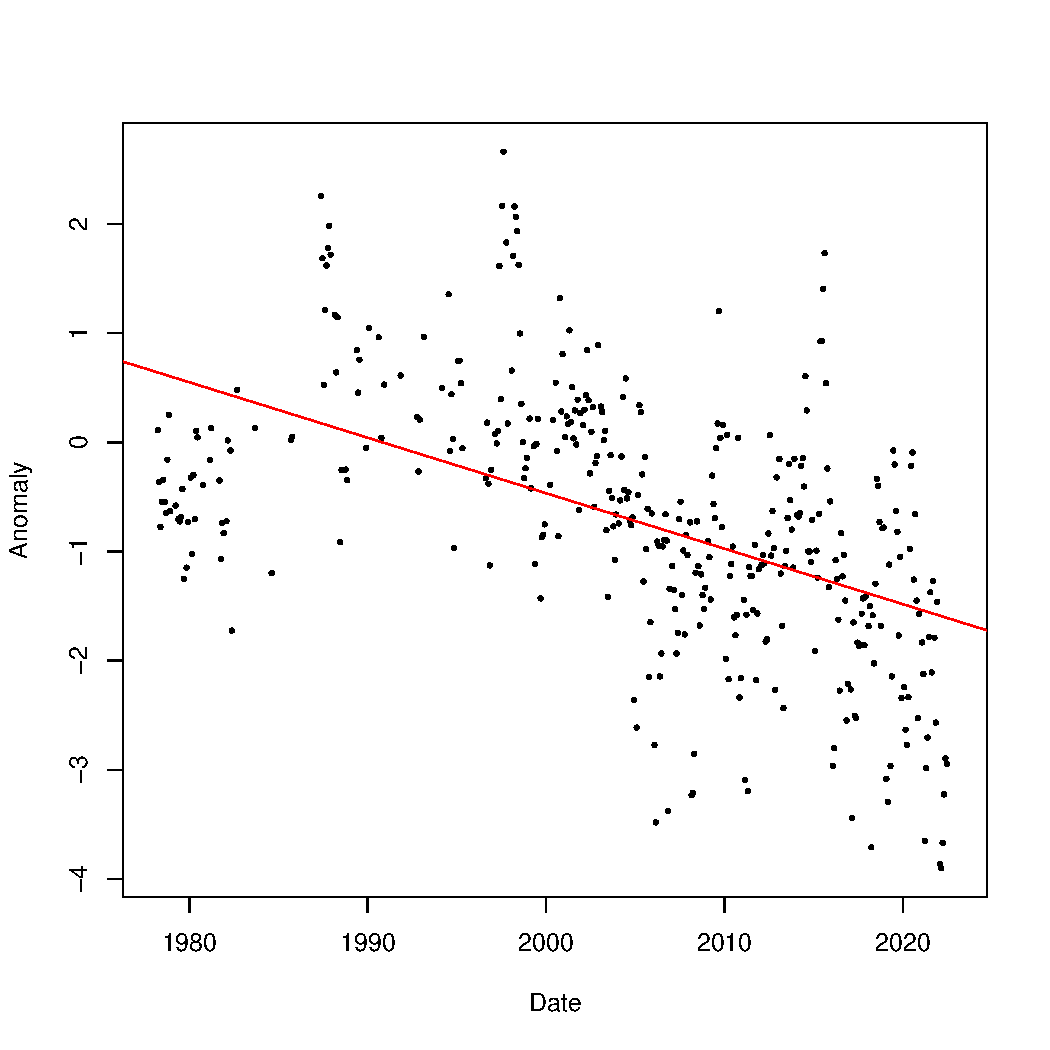
\includegraphics[width=\maxwidth]{figure/unnamed-chunk-4-1} 
\begin{kframe}\begin{alltt}
\hlcom{#zoom = 11, scale = 2, maptype ='watercolor',}

\hlkwd{png}\hlstd{(}\hlkwd{paste0}\hlstd{(}\hlstr{"png//"}\hlstd{, fips}\hlopt{$}\hlstd{State,} \hlstr{"-"}\hlstd{, stid,} \hlstr{"-MAP.png"}\hlstd{),}
    \hlkwc{width} \hlstd{=} \hlnum{480}\hlstd{,} \hlkwc{height} \hlstd{=} \hlnum{480}\hlstd{,} \hlkwc{units} \hlstd{=} \hlstr{"px"}\hlstd{,}
    \hlkwc{pointsize} \hlstd{=} \hlnum{12}\hlstd{,} \hlkwc{bg} \hlstd{=} \hlstr{"white"}\hlstd{)}
\end{alltt}


{\ttfamily\noindent\bfseries\color{errorcolor}{\#\# Error in paste0("{}png//"{}, fips\$State, "{}-"{}, stid, "{}-MAP.png"{}): object 'stid' not found}}\begin{alltt}
\hlkwd{ggmap}\hlstd{(myMap)}\hlopt{+}
\hlkwd{geom_point}\hlstd{(}\hlkwd{aes}\hlstd{(}\hlkwc{x} \hlstd{= lon,} \hlkwc{y} \hlstd{= lat),} \hlkwc{data} \hlstd{= station.df,}
   \hlkwc{alpha} \hlstd{=} \hlnum{.5}\hlstd{,} \hlkwc{color}\hlstd{=}\hlstr{"darkred"}\hlstd{,} \hlkwc{size} \hlstd{=} \hlnum{3}\hlstd{)} \hlopt{+}
   \hlkwd{geom_text}\hlstd{(}\hlkwd{aes}\hlstd{(}\hlkwc{x} \hlstd{= lon,} \hlkwc{y} \hlstd{= lat,} \hlkwc{label}\hlstd{=Station),}
      \hlkwc{data} \hlstd{= station.df,} \hlkwc{alpha} \hlstd{=} \hlnum{.5}\hlstd{,} \hlkwc{color}\hlstd{=}\hlstr{"darkred"}\hlstd{,}
      \hlkwc{size} \hlstd{=} \hlnum{3}\hlstd{,} \hlkwc{hjust}\hlstd{=}\hlnum{.1}\hlstd{,} \hlkwc{vjust}\hlstd{=}\hlopt{-}\hlnum{1}\hlstd{)}
\end{alltt}
\end{kframe}
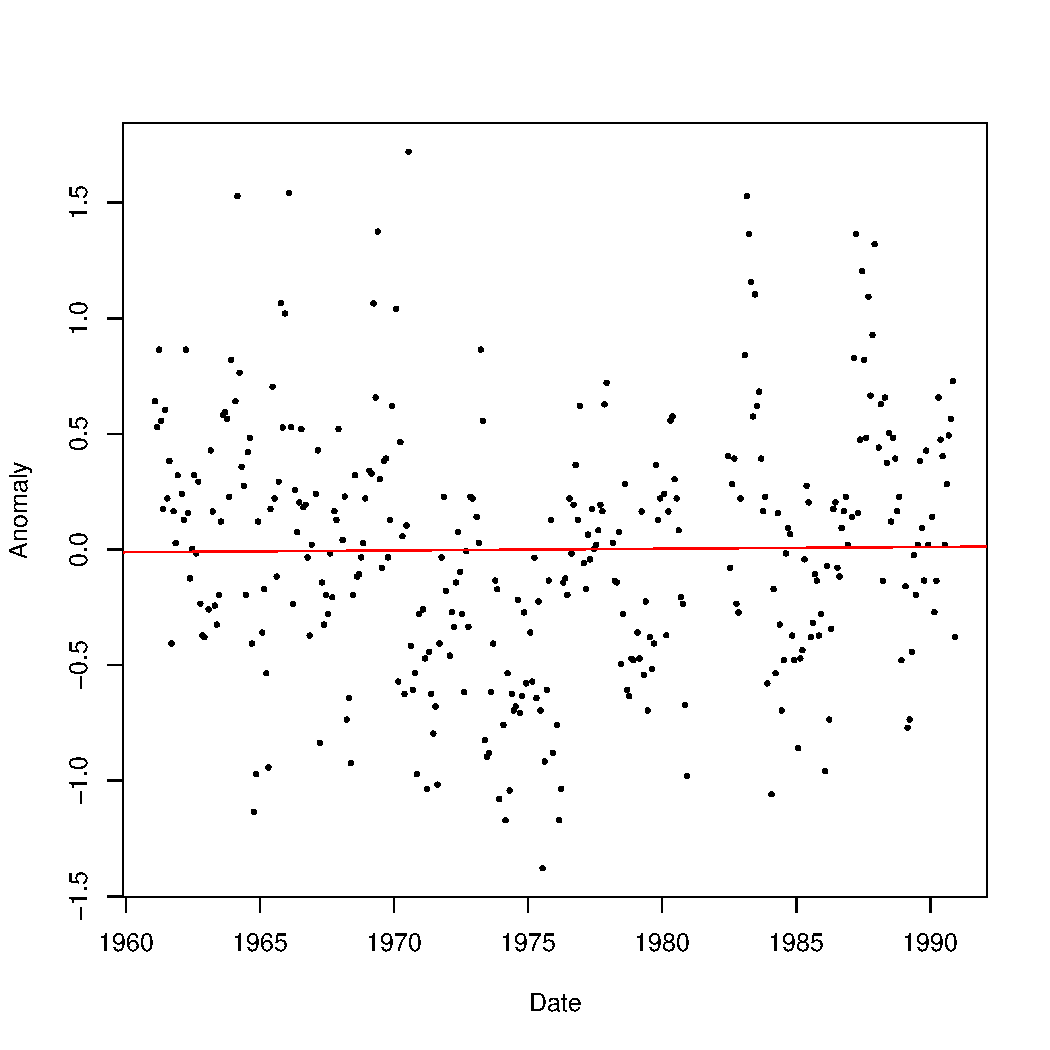
\includegraphics[width=\maxwidth]{figure/unnamed-chunk-4-2} 
\begin{kframe}\begin{alltt}
\hlkwd{dev.off}\hlstd{()}
\end{alltt}
\begin{verbatim}
## null device 
##           1
\end{verbatim}
\end{kframe}
\end{knitrout}

\begin{knitrout}
\definecolor{shadecolor}{rgb}{0.969, 0.969, 0.969}\color{fgcolor}\begin{kframe}
\begin{alltt}
\hlcom{#A) Download the main crime incident dataset}

\hlstd{incidents}\hlkwb{=} \hlkwd{read.csv}\hlstd{(}\hlstr{'https://raw.githubusercontent.com/lgellis/MiscTutorial/master/ggmap/i2Sample.csv'}\hlstd{,} \hlkwc{stringsAsFactors} \hlstd{=} \hlnum{FALSE}\hlstd{)}

\hlcom{#B) Download the extra dataset with the most dangerous Seattle cities as per:}

\hlcom{# https://housely.com/dangerous-neighborhoods-seattle/}

\hlstd{n} \hlkwb{<-} \hlkwd{read.csv}\hlstd{(}\hlstr{'https://raw.githubusercontent.com/lgellis/MiscTutorial/master/ggmap/n.csv'}\hlstd{,} \hlkwc{stringsAsFactors} \hlstd{=} \hlnum{FALSE}\hlstd{)}

\hlcom{# Look at the data sets}

\hlkwd{dim}\hlstd{(incidents)}
\hlkwd{head}\hlstd{(incidents)}
\hlkwd{attach}\hlstd{(incidents)}

\hlkwd{dim}\hlstd{(n)}
\hlkwd{head}\hlstd{(n)}
\hlkwd{attach}\hlstd{(n)}

\hlcom{# Create some color variables for graphing later}
\hlstd{col1} \hlkwb{=} \hlstr{"#011f4b"}\hlstd{; col2} \hlkwb{=} \hlstr{"#6497b1"}\hlstd{; col3} \hlkwb{=} \hlstr{"#b3cde0"}\hlstd{; col4} \hlkwb{=} \hlstr{"#CC0000"}

\hlcom{#add year to the incidents data frame}
\hlstd{incidents}\hlopt{$}\hlstd{ymd} \hlkwb{<-}\hlkwd{mdy_hms}\hlstd{(Event.Clearance.Date)}
\hlstd{incidents}\hlopt{$}\hlstd{year} \hlkwb{<-} \hlkwd{year}\hlstd{(incidents}\hlopt{$}\hlstd{ymd)}

\hlcom{#Create a more manageable data frame with only 2017 and 2018 data}
\hlstd{i2} \hlkwb{<-} \hlstd{incidents} \hlopt \hlkwd{filter}\hlstd{(year}\hlopt{>=}\hlnum{2017} \hlopt{&} \hlstd{year}\hlopt{<=}\hlnum{2018}\hlstd{)}

\hlcom{#Only include complete cases}
\hlstd{i2[}\hlkwd{complete.cases}\hlstd{(i2), ]}

\hlcom{#create a display label to the n data frame (dangerous neighbourhoods)}
\hlstd{n}\hlopt{$}\hlstd{label} \hlkwb{<-}\hlkwd{paste}\hlstd{(Rank, Location,} \hlkwc{sep}\hlstd{=}\hlstr{"-"}\hlstd{)}

\hlcom{##1) Create a map with all of the crime locations plotted.}

\hlstd{p} \hlkwb{<-} \hlkwd{ggmap}\hlstd{(}\hlkwd{get_googlemap}\hlstd{(}\hlkwc{center} \hlstd{=} \hlkwd{c}\hlstd{(}\hlkwc{lon} \hlstd{=} \hlopt{-}\hlnum{122.335167}\hlstd{,} \hlkwc{lat} \hlstd{=} \hlnum{47.608013}\hlstd{),}
                    \hlkwc{zoom} \hlstd{=} \hlnum{11}\hlstd{,} \hlkwc{scale} \hlstd{=} \hlnum{2}\hlstd{,}
                    \hlkwc{maptype} \hlstd{=}\hlstr{'terrain'}\hlstd{,}
                    \hlkwc{color} \hlstd{=} \hlstr{'color'}\hlstd{))}
\hlstd{p} \hlopt{+} \hlkwd{geom_point}\hlstd{(}\hlkwd{aes}\hlstd{(}\hlkwc{x} \hlstd{= Longitude,} \hlkwc{y} \hlstd{= Latitude,}  \hlkwc{colour} \hlstd{= Initial.Type.Group),} \hlkwc{data} \hlstd{= i2,} \hlkwc{size} \hlstd{=} \hlnum{0.5}\hlstd{)} \hlopt{+} \hlkwd{theme}\hlstd{(}\hlkwc{legend.position}\hlstd{=}\hlstr{"bottom"}\hlstd{)}
\end{alltt}
\end{kframe}
\end{knitrout}

\subsubsection{Functions to Collect and Clean GSOM}

To collect the data, I used a short function, but the download time is painfully slow because only 1 year can be obtained at a time. Might want to get a work around for this at some point. 

\begin{knitrout}
\definecolor{shadecolor}{rgb}{0.969, 0.969, 0.969}\color{fgcolor}\begin{kframe}
\begin{alltt}
\hlstd{get_GSOM} \hlkwb{<-} \hlkwa{function}\hlstd{(}\hlkwc{stid}\hlstd{,} \hlkwc{datatype}\hlstd{) \{}
   \hlstd{wtr}\hlkwb{<-}\hlkwd{list}\hlstd{()}  \hlcom{# create an empty list}
   \hlkwa{for} \hlstd{(i} \hlkwa{in} \hlstd{startyear}\hlopt{:}\hlnum{2021}\hlstd{) \{}
      \hlstd{start_date} \hlkwb{<-} \hlkwd{paste0}\hlstd{(i,} \hlstr{"-01-01"}\hlstd{)}
      \hlstd{end_date} \hlkwb{<-} \hlkwd{paste0}\hlstd{(i,} \hlstr{"-12-31"}\hlstd{)}

\hlcom{#save data portion to the list (elements named for the year}
      \hlstd{wtr[[}\hlkwd{as.character}\hlstd{(i)]]} \hlkwb{<-} \hlkwd{ncdc}\hlstd{(}\hlkwc{datasetid}\hlstd{=}\hlstr{'GSOM'}\hlstd{,}
         \hlkwc{stationid}\hlstd{=stid,} \hlkwc{datatypeid}\hlstd{=datatype,} \hlkwc{startdate} \hlstd{=}
         \hlstd{start_date,} \hlkwc{enddate} \hlstd{= end_date,} \hlkwc{limit}\hlstd{=}\hlnum{400}\hlstd{)}\hlopt{$}\hlstd{data}
   \hlstd{\}}
   \hlcom{#return the full list of data frames}
   \hlkwd{return}\hlstd{(wtr)}
\hlstd{\}}

\hlstd{stid} \hlkwb{=} \hlkwd{substr}\hlstd{(GSOM_Longest}\hlopt{$}\hlstd{id,} \hlnum{7}\hlstd{,} \hlnum{17}\hlstd{)}

\hlstd{get_GSOM2} \hlkwb{<-} \hlkwa{function}\hlstd{(}\hlkwc{stid}\hlstd{)\{}
   \hlstd{http.csv} \hlkwb{<-} \hlstr{"https://www.ncei.noaa.gov/data/global-summary-of-the-month/access/"}
   \hlkwd{read.csv}\hlstd{(}\hlkwd{paste}\hlstd{(http.csv, stid,} \hlstr{".csv"}\hlstd{,} \hlkwc{sep}\hlstd{=}\hlstr{""}\hlstd{))}
\hlstd{\}}

\hlcom{# GSOM <- get_GSOM2(stid)}
\end{alltt}
\end{kframe}
\end{knitrout}

Functions to bin data into decades and scores. 

\begin{knitrout}
\definecolor{shadecolor}{rgb}{0.969, 0.969, 0.969}\color{fgcolor}\begin{kframe}
\begin{alltt}
\hlstd{floor_decade} \hlkwb{<-} \hlkwa{function}\hlstd{(}\hlkwc{value}\hlstd{)\{}
   \hlkwd{return}\hlstd{(value} \hlopt{-} \hlstd{value} \hlopt \hlnum{10}\hlstd{) \}}
\hlcom{# Test Function}
\hlkwd{floor_decade}\hlstd{(}\hlkwd{c}\hlstd{(}\hlnum{1883}\hlstd{,}\hlnum{1988}\hlstd{))}
\end{alltt}
\begin{verbatim}
## [1] 1880 1980
\end{verbatim}
\begin{alltt}
\hlstd{floor_score} \hlkwb{<-} \hlkwa{function}\hlstd{(}\hlkwc{value}\hlstd{)\{}
   \hlkwd{return}\hlstd{(value} \hlopt{-} \hlstd{value} \hlopt \hlnum{20}\hlstd{) \}}

\hlcom{# Test Function}
\hlkwd{floor_score}\hlstd{(}\hlkwd{c}\hlstd{(}\hlnum{1883}\hlstd{,}\hlnum{1893}\hlstd{,}\hlnum{1910}\hlstd{,} \hlnum{1932}\hlstd{,}\hlnum{1940}\hlstd{))}
\end{alltt}
\begin{verbatim}
## [1] 1880 1880 1900 1920 1940
\end{verbatim}
\end{kframe}
\end{knitrout}

The function relies on two inputs, the station id and the measured parameter -- TMAX and TMIN in this case. After that, the data needs to be clean up quite a bit. 

Furthermore, I have converted units to Farenheit, which is not my favorite, but important for US consumption.

\begin{knitrout}
\definecolor{shadecolor}{rgb}{0.969, 0.969, 0.969}\color{fgcolor}\begin{kframe}
\begin{alltt}
\hlstd{GSOM_TMAX} \hlkwb{<-} \hlkwd{get_GSOM}\hlstd{(GSOM_Longest}\hlopt{$}\hlstd{id,} \hlstr{'TMAX'}\hlstd{)}
\hlstd{GSOM_TMIN} \hlkwb{<-} \hlkwd{get_GSOM}\hlstd{(GSOM_Longest}\hlopt{$}\hlstd{id,} \hlstr{'TMIN'}\hlstd{)}
\hlstd{GSOM_PPT}  \hlkwb{<-} \hlkwd{get_GSOM}\hlstd{(GSOM_Longest}\hlopt{$}\hlstd{id,} \hlstr{'PRCP'}\hlstd{)}

\hlcom{# Bind the dataframes in the list }
\hlcom{# together into one large dataframe}

\hlstd{tbl_TMAX} \hlkwb{<-} \hlstd{dplyr}\hlopt{::}\hlkwd{bind_rows}\hlstd{(GSOM_TMAX)}
\hlstd{tbl_TMIN} \hlkwb{<-} \hlstd{dplyr}\hlopt{::}\hlkwd{bind_rows}\hlstd{(GSOM_TMIN)}
\hlstd{tbl_PPT} \hlkwb{<-} \hlstd{dplyr}\hlopt{::}\hlkwd{bind_rows}\hlstd{(GSOM_PPT)}

\hlkwd{class}\hlstd{(tbl_TMAX)} \hlcom{# [1] "tbl_df"  "tbl" "data.frame"}
\end{alltt}
\begin{verbatim}
## [1] "tbl_df"     "tbl"        "data.frame"
\end{verbatim}
\begin{alltt}
\hlstd{dfTbl_TMAX} \hlkwb{=} \hlkwd{as.data.frame}\hlstd{(tbl_TMAX)}
\hlstd{dfTbl_TMIN} \hlkwb{=} \hlkwd{as.data.frame}\hlstd{(tbl_TMIN)}
\hlstd{dfTbl_PPT} \hlkwb{=} \hlkwd{as.data.frame}\hlstd{(tbl_PPT)}

\hlkwd{class}\hlstd{(dfTbl_TMAX)} \hlcom{# [1] "data.frame"}
\end{alltt}
\begin{verbatim}
## [1] "data.frame"
\end{verbatim}
\begin{alltt}
\hlstd{dfTbl_TMAX}\hlopt{$}\hlstd{TMAX} \hlkwb{=} \hlstd{dfTbl_TMAX}\hlopt{$}\hlstd{value}\hlopt{*}\hlnum{9}\hlopt{/}\hlnum{5}\hlopt{+}\hlnum{32}
\hlstd{dfTbl_TMIN}\hlopt{$}\hlstd{TMIN} \hlkwb{=} \hlstd{dfTbl_TMIN}\hlopt{$}\hlstd{value}\hlopt{*}\hlnum{9}\hlopt{/}\hlnum{5}\hlopt{+}\hlnum{32}
\hlstd{dfTbl_PPT}\hlopt{$}\hlstd{PPT} \hlkwb{=} \hlstd{dfTbl_PPT}\hlopt{$}\hlstd{value}

\hlstd{dfTbl_TMAX}\hlopt{$}\hlstd{Date} \hlkwb{=} \hlkwd{as.Date}\hlstd{(dfTbl_TMAX}\hlopt{$}\hlstd{date)}
\hlstd{dfTbl_TMIN}\hlopt{$}\hlstd{Date} \hlkwb{=} \hlkwd{as.Date}\hlstd{(dfTbl_TMIN}\hlopt{$}\hlstd{date)}
\hlstd{dfTbl_PPT}\hlopt{$}\hlstd{Date} \hlkwb{=} \hlkwd{as.Date}\hlstd{(dfTbl_PPT}\hlopt{$}\hlstd{date)}

\hlstd{dfTbl_TMAX} \hlkwb{<-} \hlkwd{subset}\hlstd{(dfTbl_TMAX,} \hlkwc{select}\hlstd{=}\hlkwd{c}\hlstd{(Date, station, TMAX))}
\hlstd{dfTbl_TMIN} \hlkwb{<-} \hlkwd{subset}\hlstd{(dfTbl_TMIN,} \hlkwc{select}\hlstd{=}\hlkwd{c}\hlstd{(Date, TMIN))}
\hlstd{dfTbl_PPT} \hlkwb{<-} \hlkwd{subset}\hlstd{(dfTbl_PPT,} \hlkwc{select}\hlstd{=}\hlkwd{c}\hlstd{(Date, PPT))}

\hlstd{dfTbl_TMAX[}\hlnum{1}\hlstd{,]}
\end{alltt}
\begin{verbatim}
##         Date           station  TMAX
## 1 1893-09-01 GHCND:USC00018024 83.75
\end{verbatim}
\begin{alltt}
\hlstd{GSOM} \hlkwb{<-} \hlkwd{merge}\hlstd{(dfTbl_TMAX, dfTbl_TMIN,} \hlkwc{by}\hlstd{=}\hlstr{"Date"}\hlstd{)}
\hlstd{GSOM} \hlkwb{<-} \hlkwd{merge}\hlstd{(GSOM, dfTbl_PPT,} \hlkwc{by}\hlstd{=}\hlstr{"Date"}\hlstd{)}

\hlstd{GSOM}\hlopt{$}\hlstd{Month} \hlkwb{=} \hlkwd{as.numeric}\hlstd{(}\hlkwd{format}\hlstd{(}\hlkwd{as.Date}\hlstd{(GSOM}\hlopt{$}\hlstd{Date),} \hlkwc{format} \hlstd{=} \hlstr{"%m"}\hlstd{))}
\hlstd{GSOM}\hlopt{$}\hlstd{Year} \hlkwb{=} \hlkwd{as.numeric}\hlstd{(}\hlkwd{format}\hlstd{(}\hlkwd{as.Date}\hlstd{(GSOM}\hlopt{$}\hlstd{Date),} \hlkwc{format} \hlstd{=} \hlstr{"%Y"}\hlstd{))}
\hlstd{GSOM}\hlopt{$}\hlstd{Decade} \hlkwb{=} \hlkwd{floor_decade}\hlstd{(GSOM}\hlopt{$}\hlstd{Year)}
\hlstd{GSOM}\hlopt{$}\hlstd{Score} \hlkwb{=} \hlkwd{floor_score}\hlstd{(GSOM}\hlopt{$}\hlstd{Year)}

\hlcom{#seq(min(GSOM$Year))}

\hlkwd{str}\hlstd{(GSOM)}
\end{alltt}
\begin{verbatim}
## 'data.frame':	1369 obs. of  9 variables:
##  $ Date   : Date, format: "1894-08-01" ...
##  $ station: chr  "GHCND:USC00018024" "GHCND:USC00018024" "GHCND:USC00018024" "GHCND:USC00018024" ...
##  $ TMAX   : num  87.8 56.2 69 68.5 87.2 ...
##  $ TMIN   : num  69.8 34.5 49.5 45.7 59.7 ...
##  $ PPT    : num  213.4 19.6 99.8 127.6 7.6 ...
##  $ Month  : num  8 2 3 4 5 6 7 8 9 10 ...
##  $ Year   : num  1894 1898 1898 1898 1898 ...
##  $ Decade : num  1890 1890 1890 1890 1890 1890 1890 1890 1890 1890 ...
##  $ Score  : num  1880 1880 1880 1880 1880 1880 1880 1880 1880 1880 ...
\end{verbatim}
\end{kframe}
\end{knitrout}

\subsubsection{Function to Evaluate Monthy Trends}

Function to evaluate each month and determine if there is a trend. At somepoint, I'll have to the stats correcting for the autocorrelation. 



Evaluate both TMAX and TMIN in GSOM by Year using MonthEvalStats() function. 
\begin{knitrout}
\definecolor{shadecolor}{rgb}{0.969, 0.969, 0.969}\color{fgcolor}\begin{kframe}
\begin{alltt}
\hlstd{MonthEvalStatsOLD} \hlkwb{<-} \hlkwa{function}\hlstd{(}\hlkwc{GSOM}\hlstd{) \{}
\hlstd{sumstats} \hlkwb{=} \hlnum{NA}
\hlkwa{for} \hlstd{(m} \hlkwa{in} \hlnum{1}\hlopt{:}\hlnum{12}\hlstd{)\{}
  \hlstd{TMIN.lm} \hlkwb{=} \hlkwd{lm}\hlstd{(TMIN}\hlopt{~}\hlstd{Date, GSOM[GSOM}\hlopt{$}\hlstd{Month}\hlopt{==}\hlstd{m,])}
  \hlstd{TMAX.lm} \hlkwb{=} \hlkwd{lm}\hlstd{(TMAX}\hlopt{~}\hlstd{Date, GSOM[GSOM}\hlopt{$}\hlstd{Month}\hlopt{==}\hlstd{m,])}
   \hlstd{PPT.lm}  \hlkwb{=} \hlkwd{lm}\hlstd{(PPT}\hlopt{~}\hlstd{Date, GSOM[GSOM}\hlopt{$}\hlstd{Month}\hlopt{==}\hlstd{m,])}

 \hlstd{sumstats} \hlkwb{=} \hlkwd{rbind}\hlstd{(sumstats,}
   \hlkwd{data.frame}\hlstd{(}\hlkwc{Month} \hlstd{= m,} \hlkwc{Param}\hlstd{=}\hlstr{"TMIN"}\hlstd{,} \hlkwc{Slope} \hlstd{=} \hlkwd{coef}\hlstd{(TMIN.lm)[}\hlnum{2}\hlstd{],}
   \hlkwc{r2} \hlstd{=} \hlkwd{summary}\hlstd{(TMIN.lm)}\hlopt{$}\hlstd{r.squared,} \hlkwc{p_value}\hlstd{=} \hlkwd{anova}\hlstd{(TMIN.lm)}\hlopt{$}\hlstr{'Pr(>F)'}\hlstd{[}\hlnum{1}\hlstd{]),}
   \hlkwd{data.frame}\hlstd{(}\hlkwc{Month} \hlstd{= m,} \hlkwc{Param}\hlstd{=}\hlstr{"TMAX"}\hlstd{,} \hlkwc{Slope} \hlstd{=} \hlkwd{coef}\hlstd{(TMAX.lm)[}\hlnum{2}\hlstd{],}
   \hlkwc{r2} \hlstd{=} \hlkwd{summary}\hlstd{(TMAX.lm)}\hlopt{$}\hlstd{r.squared,} \hlkwc{p_value}\hlstd{=} \hlkwd{anova}\hlstd{(TMAX.lm)}\hlopt{$}\hlstr{'Pr(>F)'}\hlstd{[}\hlnum{1}\hlstd{]),}
   \hlkwd{data.frame}\hlstd{(}\hlkwc{Month}\hlstd{= m,} \hlkwc{Param}\hlstd{=}\hlstr{"PPT"}\hlstd{,} \hlkwc{Slope} \hlstd{=} \hlkwd{coef}\hlstd{(PPT.lm)[}\hlnum{2}\hlstd{],}
   \hlkwc{r2} \hlstd{=} \hlkwd{summary}\hlstd{(PPT.lm)}\hlopt{$}\hlstd{r.squared,} \hlkwc{p_value}\hlstd{=} \hlkwd{anova}\hlstd{(PPT.lm)}\hlopt{$}\hlstr{'Pr(>F)'}\hlstd{[}\hlnum{1}\hlstd{]))}

\hlstd{\}}

\hlstd{sumstats}\hlkwb{=}\hlkwd{data.frame}\hlstd{(sumstats)[}\hlopt{-}\hlnum{1}\hlstd{,]}
\hlkwd{rownames}\hlstd{(sumstats)}\hlkwb{<-}\hlkwa{NULL}

\hlstd{sumstats}\hlopt{$}\hlstd{Symbol} \hlkwb{=} \hlstr{""}
\hlstd{sumstats}\hlopt{$}\hlstd{Symbol[sumstats}\hlopt{$}\hlstd{p_value} \hlopt{<} \hlnum{0.05}\hlstd{]} \hlkwb{=} \hlstr{"*"}
\hlstd{sumstats}\hlopt{$}\hlstd{Symbol[sumstats}\hlopt{$}\hlstd{p_value} \hlopt{<} \hlnum{0.01}\hlstd{]} \hlkwb{=} \hlstr{"**"}
\hlstd{sumstats}\hlopt{$}\hlstd{Symbol[sumstats}\hlopt{$}\hlstd{p_value} \hlopt{<} \hlnum{0.001}\hlstd{]} \hlkwb{=} \hlstr{"***"}
\hlstd{sumstats[,}\hlkwd{c}\hlstd{(}\hlnum{7}\hlstd{,}\hlnum{9}\hlstd{)]}
\hlkwd{return}\hlstd{(sumstats)}
\hlstd{\}}

\hlstd{MonthEvalStats} \hlkwb{<-} \hlkwa{function}\hlstd{(}\hlkwc{GSOM}\hlstd{) \{}
\hlstd{sumstats} \hlkwb{=} \hlnum{NA}
\hlkwa{for} \hlstd{(m} \hlkwa{in} \hlnum{1}\hlopt{:}\hlnum{12}\hlstd{)\{}
  \hlstd{TMIN.lm} \hlkwb{=} \hlkwd{lm}\hlstd{(TMIN}\hlopt{~}\hlstd{Date, GSOM[GSOM}\hlopt{$}\hlstd{Month}\hlopt{==}\hlstd{m,])}
  \hlstd{TMAX.lm} \hlkwb{=} \hlkwd{lm}\hlstd{(TMAX}\hlopt{~}\hlstd{Date, GSOM[GSOM}\hlopt{$}\hlstd{Month}\hlopt{==}\hlstd{m,])}
   \hlstd{PPT.lm}  \hlkwb{=} \hlkwd{lm}\hlstd{(PPT}\hlopt{~}\hlstd{Date, GSOM[GSOM}\hlopt{$}\hlstd{Month}\hlopt{==}\hlstd{m,])}

 \hlstd{sumstats} \hlkwb{=} \hlkwd{rbind}\hlstd{(sumstats,}
   \hlkwd{data.frame}\hlstd{(}\hlkwc{Month} \hlstd{= m,} \hlkwc{Param}\hlstd{=}\hlstr{"TMIN"}\hlstd{,} \hlkwc{Slope} \hlstd{=} \hlkwd{coef}\hlstd{(TMIN.lm)[}\hlnum{2}\hlstd{],}
   \hlkwc{r2} \hlstd{=} \hlkwd{summary}\hlstd{(TMIN.lm)}\hlopt{$}\hlstd{r.squared,} \hlkwc{p_value}\hlstd{=} \hlkwd{anova}\hlstd{(TMIN.lm)}\hlopt{$}\hlstr{'Pr(>F)'}\hlstd{[}\hlnum{1}\hlstd{]),}
   \hlkwd{data.frame}\hlstd{(}\hlkwc{Month} \hlstd{= m,} \hlkwc{Param}\hlstd{=}\hlstr{"TMAX"}\hlstd{,} \hlkwc{Slope} \hlstd{=} \hlkwd{coef}\hlstd{(TMAX.lm)[}\hlnum{2}\hlstd{],}
   \hlkwc{r2} \hlstd{=} \hlkwd{summary}\hlstd{(TMAX.lm)}\hlopt{$}\hlstd{r.squared,} \hlkwc{p_value}\hlstd{=} \hlkwd{anova}\hlstd{(TMAX.lm)}\hlopt{$}\hlstr{'Pr(>F)'}\hlstd{[}\hlnum{1}\hlstd{]),}
   \hlkwd{data.frame}\hlstd{(}\hlkwc{Month}\hlstd{= m,} \hlkwc{Param}\hlstd{=}\hlstr{"PPT"}\hlstd{,} \hlkwc{Slope} \hlstd{=} \hlkwd{coef}\hlstd{(PPT.lm)[}\hlnum{2}\hlstd{],}
   \hlkwc{r2} \hlstd{=} \hlkwd{summary}\hlstd{(PPT.lm)}\hlopt{$}\hlstd{r.squared,} \hlkwc{p_value}\hlstd{=} \hlkwd{anova}\hlstd{(PPT.lm)}\hlopt{$}\hlstr{'Pr(>F)'}\hlstd{[}\hlnum{1}\hlstd{]))}

\hlstd{\}} \hlcom{#end loop}

\hlstd{sumstats}\hlkwb{=}\hlkwd{data.frame}\hlstd{(sumstats)[}\hlopt{-}\hlnum{1}\hlstd{,]}
\hlkwd{rownames}\hlstd{(sumstats)}\hlkwb{<-}\hlkwa{NULL}
\hlkwd{head}\hlstd{(sumstats)}

\hlstd{sumstats}\hlopt{$}\hlstd{Symbol} \hlkwb{=} \hlstr{""}
\hlstd{sumstats}\hlopt{$}\hlstd{Symbol[sumstats}\hlopt{$}\hlstd{p_value} \hlopt{<} \hlnum{0.05}\hlstd{]} \hlkwb{=} \hlstr{"*"}
\hlstd{sumstats}\hlopt{$}\hlstd{Symbol[sumstats}\hlopt{$}\hlstd{p_value} \hlopt{<} \hlnum{0.01}\hlstd{]} \hlkwb{=} \hlstr{"**"}
\hlstd{sumstats}\hlopt{$}\hlstd{Symbol[sumstats}\hlopt{$}\hlstd{p_value} \hlopt{<} \hlnum{0.001}\hlstd{]} \hlkwb{=} \hlstr{"***"}
\hlkwd{return}\hlstd{(sumstats)}
\hlstd{\}}

\hlcom{# test function}
\hlstd{sumstats} \hlkwb{=} \hlkwd{MonthEvalStats}\hlstd{(GSOM[}\hlnum{500}\hlopt{:}\hlnum{4000}\hlstd{,])}
\end{alltt}
\end{kframe}
\end{knitrout}

\subsubsection{Function to report Probabilities}

\begin{knitrout}
\definecolor{shadecolor}{rgb}{0.969, 0.969, 0.969}\color{fgcolor}\begin{kframe}
\begin{alltt}
\hlstd{report_prob} \hlkwb{<-}\hlkwa{function}\hlstd{(}\hlkwc{pvalue}\hlstd{)\{}
   \hlkwa{if}\hlstd{(pvalue} \hlopt{>} \hlnum{0.05}\hlstd{)} \hlkwd{return}\hlstd{(}\hlstr{"> 0.05 (Not Significant)"}\hlstd{)}
   \hlkwa{if}\hlstd{(pvalue} \hlopt{<} \hlnum{0.05} \hlopt{&} \hlstd{pvalue} \hlopt{>=} \hlnum{0.001}\hlstd{)} \hlkwd{return}\hlstd{(}
      \hlkwd{paste}\hlstd{(}\hlstr{"="}\hlstd{,} \hlkwd{round}\hlstd{(pvalue,} \hlnum{3}\hlstd{),} \hlstr{"(Statistically Significant)"}\hlstd{))}
   \hlcom{#if(pvalue < 0.01) print(round(pvalue, 4))}
   \hlkwa{if}\hlstd{(pvalue} \hlopt{<} \hlnum{0.001}\hlstd{)} \hlkwd{return}\hlstd{(}\hlstr{"< 0.001 (Statisically Significant)"}\hlstd{)}
\hlstd{\}}

\hlcom{#test function}
\hlkwd{report_prob}\hlstd{(}\hlnum{0.0032}\hlstd{)}

\hlstd{report_prob2} \hlkwb{<-}\hlkwa{function}\hlstd{(}\hlkwc{lm}\hlstd{)\{}
   \hlcom{# lm=GSOM.lm}
   \hlkwa{if}\hlstd{(}\hlkwd{anova}\hlstd{(lm)}\hlopt{$}\hlstr{'Pr(>F)'}\hlstd{[}\hlnum{1}\hlstd{]} \hlopt{>} \hlnum{0.05}\hlstd{)\{}
         \hlkwd{return}\hlstd{(}\hlstr{"p-value > 0.05 (Not Significant)"}\hlstd{)}
      \hlstd{\}}
   \hlkwa{if}\hlstd{(}\hlkwd{anova}\hlstd{(lm)}\hlopt{$}\hlstr{'Pr(>F)'}\hlstd{[}\hlnum{1}\hlstd{]} \hlopt{<} \hlnum{0.05} \hlopt{&}
      \hlkwd{anova}\hlstd{(lm)}\hlopt{$}\hlstr{'Pr(>F)'}\hlstd{[}\hlnum{1}\hlstd{]} \hlopt{>=} \hlnum{0.001}\hlstd{)\{}
         \hlkwd{return}\hlstd{(}\hlkwd{paste}\hlstd{(}\hlstr{"Change "}\hlstd{,} \hlkwd{round}\hlstd{(}\hlkwd{coef}\hlstd{(lm)[}\hlnum{2}\hlstd{]}\hlopt{*}\hlnum{356.25}\hlopt{*}\hlnum{100}\hlstd{,} \hlnum{1}\hlstd{),}
         \hlstr{"/100 years, "}\hlstd{,} \hlstr{"p-value ="}\hlstd{,} \hlkwd{round}\hlstd{(}\hlkwd{anova}\hlstd{(lm)}\hlopt{$}\hlstr{'Pr(>F)'}\hlstd{[}\hlnum{1}\hlstd{],} \hlnum{3}\hlstd{),}
         \hlstr{"(Statistically Significant)"}\hlstd{,} \hlkwc{sep}\hlstd{=}\hlstr{""}\hlstd{))}
      \hlstd{\}}
   \hlkwa{if}\hlstd{(}\hlkwd{anova}\hlstd{(lm)}\hlopt{$}\hlstr{'Pr(>F)'}\hlstd{[}\hlnum{1}\hlstd{]} \hlopt{<} \hlnum{0.001}\hlstd{) \{}
         \hlkwd{return}\hlstd{(}\hlkwd{paste}\hlstd{(}\hlstr{"Change "}\hlstd{,} \hlkwd{round}\hlstd{(}\hlkwd{coef}\hlstd{(lm)[}\hlnum{2}\hlstd{]}\hlopt{*}\hlnum{325.25}\hlopt{*}\hlnum{100}\hlstd{,} \hlnum{1}\hlstd{),}
         \hlstr{"/100 years, "}\hlstd{,} \hlstr{"p-value < 0.001 (Statistically Significant)"}\hlstd{,}
         \hlkwc{sep}\hlstd{=}\hlstr{""}\hlstd{))}
   \hlstd{\}}
\hlstd{\}}

\hlstd{report_prob3} \hlkwb{<-}\hlkwa{function}\hlstd{(}\hlkwc{lm}\hlstd{)\{}
   \hlcom{#lm=Drought.run.lm}
   \hlstd{temp} \hlkwb{=} \hlkwd{data.frame}\hlstd{(}\hlkwc{change} \hlstd{=} \hlnum{NA}\hlstd{,} \hlkwc{p_value}\hlstd{=}\hlnum{NA}\hlstd{,} \hlkwc{note}\hlstd{=}\hlnum{NA}\hlstd{)}
   \hlkwa{if}\hlstd{(}\hlkwd{anova}\hlstd{(lm)}\hlopt{$}\hlstr{'Pr(>F)'}\hlstd{[}\hlnum{1}\hlstd{]} \hlopt{>} \hlnum{0.05}\hlstd{)\{}
      \hlstd{temp[,}\hlnum{1}\hlstd{]} \hlkwb{<-} \hlstr{""}\hlstd{;}
      \hlstd{temp[,}\hlnum{2}\hlstd{]} \hlkwb{<-} \hlstr{"p-value > 0.05"}\hlstd{;}
      \hlstd{temp[,}\hlnum{3}\hlstd{]} \hlkwb{<-} \hlstr{"(Not Significant)"}
      \hlkwd{return}\hlstd{(temp)}
      \hlstd{\}}
   \hlkwa{if}\hlstd{(}\hlkwd{anova}\hlstd{(lm)}\hlopt{$}\hlstr{'Pr(>F)'}\hlstd{[}\hlnum{1}\hlstd{]} \hlopt{<} \hlnum{0.05} \hlopt{&}
      \hlkwd{anova}\hlstd{(lm)}\hlopt{$}\hlstr{'Pr(>F)'}\hlstd{[}\hlnum{1}\hlstd{]} \hlopt{>=} \hlnum{0.001}\hlstd{)\{}
      \hlstd{temp[,}\hlnum{1}\hlstd{]} \hlkwb{<-} \hlkwd{paste}\hlstd{(}\hlstr{"Change: "}\hlstd{,}
         \hlkwd{round}\hlstd{(}\hlkwd{coef}\hlstd{(lm)[}\hlnum{2}\hlstd{]}\hlopt{*}\hlnum{356.25}\hlopt{*}\hlnum{100}\hlstd{,} \hlnum{1}\hlstd{),} \hlstr{"°F/100 years"}\hlstd{,} \hlkwc{sep}\hlstd{=}\hlstr{""}\hlstd{);}
      \hlstd{temp[,}\hlnum{2}\hlstd{]} \hlkwb{<-} \hlkwd{paste}\hlstd{(}\hlstr{"p-value = "}\hlstd{,}
         \hlkwd{round}\hlstd{(}\hlkwd{anova}\hlstd{(lm)}\hlopt{$}\hlstr{'Pr(>F)'}\hlstd{[}\hlnum{1}\hlstd{],} \hlnum{3}\hlstd{),} \hlkwc{sep}\hlstd{=}\hlstr{""}\hlstd{);}
      \hlstd{temp[,}\hlnum{3}\hlstd{]} \hlkwb{<-} \hlstr{" (Statistically Significant)"}
      \hlkwd{return}\hlstd{(temp)}
      \hlstd{\}}
   \hlkwa{if}\hlstd{(}\hlkwd{anova}\hlstd{(lm)}\hlopt{$}\hlstr{'Pr(>F)'}\hlstd{[}\hlnum{1}\hlstd{]} \hlopt{<} \hlnum{0.001}\hlstd{) \{}
      \hlstd{temp[,}\hlnum{1}\hlstd{]} \hlkwb{<-} \hlkwd{paste}\hlstd{(}\hlstr{"Change: "}\hlstd{,} \hlkwd{round}\hlstd{(}\hlkwd{coef}\hlstd{(lm)[}\hlnum{2}\hlstd{]}\hlopt{*}\hlnum{356.25}\hlopt{*}\hlnum{100}\hlstd{,} \hlnum{1}\hlstd{),} \hlstr{"°F/100 years"}\hlstd{,} \hlkwc{sep}\hlstd{=}\hlstr{""}\hlstd{);}
      \hlstd{temp[,}\hlnum{2}\hlstd{]} \hlkwb{<-} \hlstr{"p-value < 0.001"}\hlstd{;}
      \hlstd{temp[,}\hlnum{3}\hlstd{]} \hlkwb{<-} \hlstr{" (Statistically Significant)"}
      \hlkwd{return}\hlstd{(temp)}
   \hlstd{\}}
\hlstd{\}}
\end{alltt}
\end{kframe}
\end{knitrout}

\section{Communicating Long-term Weather Records}

\subsection{Complete Records vs. Post 1975 Trends}

\begin{knitrout}
\definecolor{shadecolor}{rgb}{0.969, 0.969, 0.969}\color{fgcolor}\begin{kframe}
\begin{alltt}
\hlkwd{setwd}\hlstd{(}\hlstr{"/home/CAMPUS/mwl04747/github/Climate_Change_Narratives/Social_Media"}\hlstd{)}
\hlkwd{png}\hlstd{(}\hlkwd{paste0}\hlstd{(}\hlstr{"png//"}\hlstd{, fips}\hlopt{$}\hlstd{State,} \hlstr{"-"}\hlstd{, stid,} \hlstr{"-GSOMmonthly.png"}\hlstd{),} \hlkwc{width} \hlstd{=} \hlnum{480}\hlstd{,} \hlkwc{height} \hlstd{=} \hlnum{320}\hlstd{,} \hlkwc{units} \hlstd{=} \hlstr{"px"}\hlstd{,} \hlkwc{pointsize} \hlstd{=} \hlnum{12}\hlstd{,} \hlkwc{bg} \hlstd{=} \hlstr{"white"}\hlstd{)}
\hlkwd{par}\hlstd{(}\hlkwc{las}\hlstd{=}\hlnum{1}\hlstd{,} \hlkwc{mfrow}\hlstd{=}\hlkwd{c}\hlstd{(}\hlnum{1}\hlstd{,}\hlnum{1}\hlstd{))}
\hlkwd{plot}\hlstd{(TMAX}\hlopt{~}\hlstd{Date, GSOM,} \hlkwc{pch}\hlstd{=}\hlnum{20}\hlstd{,} \hlkwc{cex}\hlstd{=}\hlnum{.5}\hlstd{,} \hlkwc{col}\hlstd{=}\hlstr{"grey"}\hlstd{,} \hlkwc{ylab}\hlstd{=}\hlstr{"°F"}\hlstd{,} \hlkwc{main}\hlstd{=}\hlkwd{paste0}\hlstd{(fips}\hlopt{$}\hlstd{State,} \hlstr{"-"}\hlstd{, stid))}
\hlstd{GSOM.lm} \hlkwb{=} \hlkwd{lm}\hlstd{(TMAX}\hlopt{~}\hlstd{Date, GSOM)}
\hlstd{pred_dates} \hlkwb{<-}\hlkwd{data.frame}\hlstd{(}\hlkwc{Date} \hlstd{= GSOM}\hlopt{$}\hlstd{Date);}
\hlkwd{nrow}\hlstd{(pred_dates);}\hlcom{# pred_dates}
\end{alltt}
\begin{verbatim}
## [1] 1369
\end{verbatim}
\begin{alltt}
\hlcom{#Predits the values with confidence interval }
\hlstd{ci} \hlkwb{<-} \hlkwd{predict}\hlstd{(GSOM.lm,} \hlkwc{newdata} \hlstd{= pred_dates,}
              \hlkwc{interval} \hlstd{=} \hlstr{'confidence'}\hlstd{)}
\hlkwd{lines}\hlstd{(pred_dates}\hlopt{$}\hlstd{Date,} \hlkwd{as.numeric}\hlstd{(ci[,}\hlnum{1}\hlstd{]),} \hlkwc{col}\hlstd{=}\hlstr{"gray50"}\hlstd{)}

\hlcom{# Post 1975}
\hlstd{GSOM.lm} \hlkwb{=} \hlkwd{lm}\hlstd{(TMAX}\hlopt{~}\hlstd{Date, GSOM[GSOM}\hlopt{$}\hlstd{Year}\hlopt{>}\hlnum{1975}\hlstd{,])}
\hlstd{pred_dates} \hlkwb{<-}\hlkwd{data.frame}\hlstd{(}\hlkwc{Date} \hlstd{= GSOM}\hlopt{$}\hlstd{Date[GSOM}\hlopt{$}\hlstd{Year}\hlopt{>}\hlnum{1975}\hlstd{]);}
\hlkwd{nrow}\hlstd{(pred_dates);} \hlcom{#pred_dates}
\end{alltt}
\begin{verbatim}
## [1] 510
\end{verbatim}
\begin{alltt}
\hlcom{#Predits the values with confidence interval }
\hlstd{ci} \hlkwb{<-} \hlkwd{predict}\hlstd{(GSOM.lm,} \hlkwc{newdata} \hlstd{= pred_dates,}
              \hlkwc{interval} \hlstd{=} \hlstr{'confidence'}\hlstd{)}
\hlkwd{lines}\hlstd{(pred_dates}\hlopt{$}\hlstd{Date,} \hlkwd{as.numeric}\hlstd{(ci[,}\hlnum{1}\hlstd{]),} \hlkwc{col}\hlstd{=}\hlstr{"red"}\hlstd{)}
\hlkwd{lines}\hlstd{(pred_dates}\hlopt{$}\hlstd{Date,} \hlkwd{as.numeric}\hlstd{(ci[,}\hlnum{2}\hlstd{]),} \hlkwc{col}\hlstd{=}\hlstr{"darkorange"}\hlstd{)}
\hlkwd{lines}\hlstd{(pred_dates}\hlopt{$}\hlstd{Date, ci[,}\hlnum{3}\hlstd{],} \hlkwc{col}\hlstd{=}\hlstr{"darkorange"}\hlstd{)}
\hlstd{location_index} \hlkwb{=} \hlkwd{round}\hlstd{(}\hlkwd{length}\hlstd{(GSOM[GSOM}\hlopt{$}\hlstd{Year}\hlopt{>}\hlnum{1975}\hlstd{,]}\hlopt{$}\hlstd{Date)} \hlopt{*} \hlnum{0.99}\hlstd{,}\hlnum{0}\hlstd{)}
\hlkwd{text}\hlstd{(pred_dates}\hlopt{$}\hlstd{Date[location_index], ci[location_index,}\hlnum{3}\hlstd{],}
     \hlkwd{paste}\hlstd{(}\hlkwd{report_prob3}\hlstd{(GSOM.lm))[}\hlnum{2}\hlstd{],} \hlkwc{pos}\hlstd{=}\hlnum{2}\hlstd{,} \hlkwc{cex}\hlstd{=}\hlnum{1.0}\hlstd{,} \hlkwc{col}\hlstd{=}\hlstr{"red"}\hlstd{)}
\hlcom{#abline(coef(lm(TMAX~Date, GSOM)), col="black")}
\hlcom{#abline(coef(lm(TMAX~Date, GSOM[GSOM$Year>1975,])), col="red")}
\hlkwd{dev.off}\hlstd{()}
\end{alltt}
\begin{verbatim}
## pdf 
##   2
\end{verbatim}
\end{kframe}
\end{knitrout}

\begin{figure}
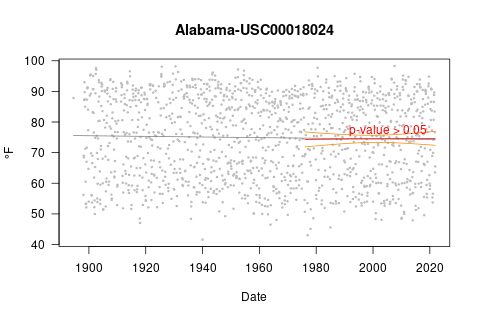
\includegraphics[width=1.00\textwidth]{/home/CAMPUS/mwl04747/github/Climate_Change_Narratives/Social_Media/png/Alabama-USC00018024-GSOMmonthly.png}
\caption{The climate trends from full record and post 1975 data. These data have a high level of variability due to seasonality effects that have not been filtered out.}
\label{fig:GSOM-1975trend}
\end{figure}

The noise in the data suggest that there is no trend, but it's tricky because the seasonal variation dominates the source of varition. Is there a way to "filter" out the seasonal effect?

\subsection{Filtering Seasonal Effect}

There are several ways to filter out seasonal effects. The easiest way is subtract the mean value for each date, but that's tricky because every four years there is an extra day in Februrary -- although there are ways to deal with this, a more straight forward way is to use mean monthly values to capture the seasonality for each month. With 12 months, this is a pretty good approach because there is pretty good resolution. 

Method 1 Filtering by Monthly Mean 

\begin{knitrout}
\definecolor{shadecolor}{rgb}{0.969, 0.969, 0.969}\color{fgcolor}\begin{kframe}
\begin{alltt}
\hlstd{TMAX.Monthly.means} \hlkwb{=} \hlkwd{aggregate}\hlstd{(TMAX}\hlopt{~}\hlstd{Month,} \hlkwc{data}\hlstd{=GSOM, mean)}
\hlkwd{names}\hlstd{(TMAX.Monthly.means)}\hlkwb{=}\hlkwd{c}\hlstd{(}\hlstr{"Month"}\hlstd{,} \hlstr{"TMAXmean"}\hlstd{)}
\hlstd{GSOM2} \hlkwb{=} \hlkwd{merge}\hlstd{(GSOM, TMAX.Monthly.means,} \hlkwc{by}\hlstd{=}\hlstr{"Month"}\hlstd{)}
\hlstd{GSOM2}\hlopt{$}\hlstd{TMAX.anom} \hlkwb{=} \hlstd{GSOM2}\hlopt{$}\hlstd{TMAX} \hlopt{-} \hlstd{GSOM2}\hlopt{$}\hlstd{TMAXmean}

\hlstd{TMIN.Monthly.means} \hlkwb{=} \hlkwd{aggregate}\hlstd{(TMIN}\hlopt{~}\hlstd{Month, GSOM, mean)}
\hlkwd{names}\hlstd{(TMIN.Monthly.means)}\hlkwb{=}\hlkwd{c}\hlstd{(}\hlstr{"Month"}\hlstd{,} \hlstr{"TMINmean"}\hlstd{)}
\hlstd{GSOM2} \hlkwb{=} \hlkwd{merge}\hlstd{(GSOM2, TMIN.Monthly.means,} \hlkwc{by}\hlstd{=}\hlstr{"Month"}\hlstd{)}
\hlstd{GSOM2}\hlopt{$}\hlstd{TMIN.anom} \hlkwb{=} \hlstd{GSOM2}\hlopt{$}\hlstd{TMIN} \hlopt{-} \hlstd{GSOM2}\hlopt{$}\hlstd{TMINmean}

\hlstd{PPT.Monthly.means} \hlkwb{=} \hlkwd{aggregate}\hlstd{(PPT}\hlopt{~}\hlstd{Month, GSOM, mean)}
\hlkwd{names}\hlstd{(PPT.Monthly.means)}\hlkwb{=}\hlkwd{c}\hlstd{(}\hlstr{"Month"}\hlstd{,} \hlstr{"PPTmean"}\hlstd{)}
\hlstd{GSOM2} \hlkwb{=} \hlkwd{merge}\hlstd{(GSOM2, PPT.Monthly.means,} \hlkwc{by}\hlstd{=}\hlstr{"Month"}\hlstd{)}
\hlstd{GSOM2}\hlopt{$}\hlstd{PPT.anom} \hlkwb{=} \hlstd{GSOM2}\hlopt{$}\hlstd{PPT} \hlopt{-} \hlstd{GSOM2}\hlopt{$}\hlstd{PPTmean}

\hlcom{# Sort by date}
\hlstd{GSOM2} \hlkwb{<-} \hlstd{GSOM2[}\hlkwd{order}\hlstd{(GSOM2}\hlopt{$}\hlstd{Date),]}
\end{alltt}
\end{kframe}
\end{knitrout}

\begin{knitrout}
\definecolor{shadecolor}{rgb}{0.969, 0.969, 0.969}\color{fgcolor}\begin{kframe}
\begin{alltt}
\hlkwd{png}\hlstd{(}\hlkwd{paste0}\hlstd{(}\hlstr{"png//"}\hlstd{, fips}\hlopt{$}\hlstd{State,} \hlstr{"-"}\hlstd{, stid,} \hlstr{"-GSOM-anomaly.png"}\hlstd{),}
    \hlkwc{width} \hlstd{=} \hlnum{480}\hlstd{,} \hlkwc{height} \hlstd{=} \hlnum{320}\hlstd{,} \hlkwc{units} \hlstd{=} \hlstr{"px"}\hlstd{,}
    \hlkwc{pointsize} \hlstd{=} \hlnum{12}\hlstd{,} \hlkwc{bg} \hlstd{=} \hlstr{"white"}\hlstd{)}
\hlkwd{par}\hlstd{(}\hlkwc{las}\hlstd{=}\hlnum{1}\hlstd{,} \hlkwc{mfrow}\hlstd{=}\hlkwd{c}\hlstd{(}\hlnum{1}\hlstd{,}\hlnum{1}\hlstd{))}
\hlkwd{par}\hlstd{(}\hlkwc{las}\hlstd{=}\hlnum{1}\hlstd{)}
\hlkwd{plot}\hlstd{(TMAX.anom}\hlopt{~}\hlstd{Date, GSOM2,} \hlkwc{pch}\hlstd{=}\hlnum{20}\hlstd{,} \hlkwc{cex}\hlstd{=}\hlnum{.5}\hlstd{,}
     \hlkwc{col}\hlstd{=}\hlstr{"grey"}\hlstd{,} \hlkwc{ylab}\hlstd{=}\hlstr{"Max. Temp (anomaly) °F"}\hlstd{,}
     \hlkwc{main}\hlstd{=}\hlkwd{paste0}\hlstd{(}\hlstr{"Seasonally Filtered"}\hlstd{, fips}\hlopt{$}\hlstd{State,} \hlstr{" ("}\hlstd{, stid,} \hlstr{")"}\hlstd{,}
         \hlkwd{report_prob3}\hlstd{(GSOM.lm)[}\hlnum{3}\hlstd{]))}
\hlstd{GSOM.lm} \hlkwb{=} \hlkwd{lm}\hlstd{(TMAX.anom}\hlopt{~}\hlstd{Date, GSOM2)}
\hlstd{pred_dates} \hlkwb{<-}\hlkwd{data.frame}\hlstd{(}\hlkwc{Date} \hlstd{= GSOM2}\hlopt{$}\hlstd{Date);}
\hlkwd{nrow}\hlstd{(pred_dates);} \hlcom{#pred_dates}
\end{alltt}
\begin{verbatim}
## [1] 1369
\end{verbatim}
\begin{alltt}
\hlcom{#Predits the values with confidence interval }
\hlstd{ci} \hlkwb{<-} \hlkwd{predict}\hlstd{(GSOM.lm,} \hlkwc{newdata} \hlstd{= pred_dates,}
              \hlkwc{interval} \hlstd{=} \hlstr{'confidence'}\hlstd{)}
\hlkwd{lines}\hlstd{(pred_dates}\hlopt{$}\hlstd{Date,} \hlkwd{as.numeric}\hlstd{(ci[,}\hlnum{1}\hlstd{]),} \hlkwc{col}\hlstd{=}\hlstr{"gray50"}\hlstd{)}

\hlstd{ymax}\hlkwb{=}\hlkwd{max}\hlstd{(GSOM2}\hlopt{$}\hlstd{TMAX.anom)} \hlopt{-} \hlstd{(}\hlkwd{max}\hlstd{(GSOM2}\hlopt{$}\hlstd{TMAX.anom)}\hlopt{-}\hlkwd{min}\hlstd{(GSOM2}\hlopt{$}\hlstd{TMAX.anom))}\hlopt{*}\hlnum{.3}
\hlstd{ymax2} \hlkwb{<-} \hlstd{ymax} \hlopt{-} \hlstd{(}\hlkwd{max}\hlstd{(GSOM2}\hlopt{$}\hlstd{TMAX.anom)}\hlopt{-}\hlkwd{min}\hlstd{(GSOM2}\hlopt{$}\hlstd{TMAX.anom))}\hlopt{*}\hlnum{.1}

\hlstd{location_index} \hlkwb{=} \hlkwd{round}\hlstd{(}\hlkwd{length}\hlstd{(GSOM2[GSOM2}\hlopt{$}\hlstd{Year}\hlopt{>}\hlnum{1975}\hlstd{,]}\hlopt{$}\hlstd{Date)} \hlopt{*} \hlnum{0.99}\hlstd{,}\hlnum{3}\hlstd{)}
\hlkwd{text}\hlstd{(pred_dates}\hlopt{$}\hlstd{Date[location_index], ymax,}
     \hlkwd{paste}\hlstd{(}\hlkwd{report_prob3}\hlstd{(GSOM.lm))[}\hlnum{1}\hlstd{],} \hlkwc{pos}\hlstd{=}\hlnum{2}\hlstd{,} \hlkwc{cex}\hlstd{=}\hlnum{.9}\hlstd{)}
\hlkwd{text}\hlstd{(pred_dates}\hlopt{$}\hlstd{Date[location_index], ymax2,}
     \hlkwd{paste}\hlstd{(}\hlkwd{report_prob3}\hlstd{(GSOM.lm))[}\hlnum{2}\hlstd{],} \hlkwc{pos}\hlstd{=}\hlnum{2}\hlstd{,} \hlkwc{cex}\hlstd{=}\hlnum{.9}\hlstd{)}

\hlcom{# Post 1975}
\hlstd{GSOM.lm} \hlkwb{=} \hlkwd{lm}\hlstd{(TMAX.anom}\hlopt{~}\hlstd{Date, GSOM2[GSOM2}\hlopt{$}\hlstd{Year}\hlopt{>}\hlnum{1975}\hlstd{,])}
\hlstd{pred_dates} \hlkwb{<-}\hlkwd{data.frame}\hlstd{(}\hlkwc{Date} \hlstd{= GSOM2}\hlopt{$}\hlstd{Date[GSOM2}\hlopt{$}\hlstd{Year}\hlopt{>}\hlnum{1975}\hlstd{]);}
\hlkwd{nrow}\hlstd{(pred_dates);} \hlcom{#pred_dates}
\end{alltt}
\begin{verbatim}
## [1] 510
\end{verbatim}
\begin{alltt}
\hlcom{#Predits the values with confidence interval }
\hlstd{ci} \hlkwb{<-} \hlkwd{predict}\hlstd{(GSOM.lm,} \hlkwc{newdata} \hlstd{= pred_dates,}
              \hlkwc{interval} \hlstd{=} \hlstr{'confidence'}\hlstd{)}
\hlkwd{lines}\hlstd{(pred_dates}\hlopt{$}\hlstd{Date,} \hlkwd{as.numeric}\hlstd{(ci[,}\hlnum{1}\hlstd{]),} \hlkwc{col}\hlstd{=}\hlstr{"red"}\hlstd{)}
\hlkwd{lines}\hlstd{(pred_dates}\hlopt{$}\hlstd{Date,} \hlkwd{as.numeric}\hlstd{(ci[,}\hlnum{2}\hlstd{]),} \hlkwc{col}\hlstd{=}\hlstr{"darkorange"}\hlstd{)}
\hlkwd{lines}\hlstd{(pred_dates}\hlopt{$}\hlstd{Date, ci[,}\hlnum{3}\hlstd{],} \hlkwc{col}\hlstd{=}\hlstr{"darkorange"}\hlstd{)}

\hlstd{ymax}\hlkwb{=}\hlkwd{max}\hlstd{(GSOM2}\hlopt{$}\hlstd{TMAX.anom)} \hlopt{-} \hlstd{(}\hlkwd{max}\hlstd{(GSOM2}\hlopt{$}\hlstd{TMAX.anom)}\hlopt{-}\hlkwd{min}\hlstd{(GSOM2}\hlopt{$}\hlstd{TMAX.anom))}\hlopt{*}\hlnum{.7}
\hlstd{ymax2} \hlkwb{<-} \hlstd{ymax} \hlopt{-} \hlstd{(}\hlkwd{max}\hlstd{(GSOM2}\hlopt{$}\hlstd{TMAX.anom)}\hlopt{-}\hlkwd{min}\hlstd{(GSOM2}\hlopt{$}\hlstd{TMAX.anom))}\hlopt{*}\hlnum{.1}

\hlstd{location_index} \hlkwb{=} \hlkwd{round}\hlstd{(}\hlkwd{length}\hlstd{(GSOM2[GSOM2}\hlopt{$}\hlstd{Year}\hlopt{>}\hlnum{1975}\hlstd{,]}\hlopt{$}\hlstd{Date)} \hlopt{*} \hlnum{0.99}\hlstd{,}\hlnum{0}\hlstd{)}
\hlkwd{text}\hlstd{(pred_dates}\hlopt{$}\hlstd{Date[location_index], ymax,}
     \hlkwd{paste}\hlstd{(}\hlkwd{report_prob3}\hlstd{(GSOM.lm))[}\hlnum{1}\hlstd{],} \hlkwc{pos}\hlstd{=}\hlnum{2}\hlstd{,} \hlkwc{cex}\hlstd{=}\hlnum{.9}\hlstd{,} \hlkwc{col}\hlstd{=}\hlstr{"red"}\hlstd{)}
\hlkwd{text}\hlstd{(pred_dates}\hlopt{$}\hlstd{Date[location_index], ymax2,}
     \hlkwd{paste}\hlstd{(}\hlkwd{report_prob3}\hlstd{(GSOM.lm))[}\hlnum{2}\hlstd{],} \hlkwc{pos}\hlstd{=}\hlnum{2}\hlstd{,} \hlkwc{cex}\hlstd{=}\hlnum{.9}\hlstd{,} \hlkwc{col}\hlstd{=}\hlstr{"red"}\hlstd{)}
\hlkwd{dev.off}\hlstd{()}
\end{alltt}
\begin{verbatim}
## pdf 
##   2
\end{verbatim}
\end{kframe}
\end{knitrout}

%"png//", fips$State, "-", stid, "-GSOM-anomoly.png"

And to see what we created, see Figure~\ref{fig:GSOM-anomaly}.

\begin{figure}
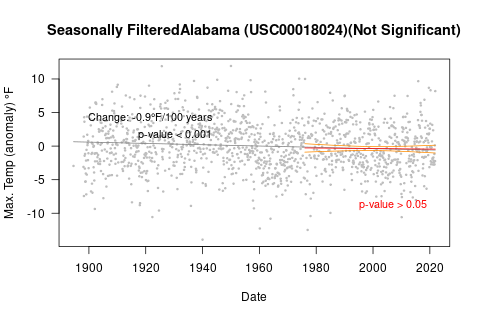
\includegraphics[width=1.00\textwidth]{/home/CAMPUS/mwl04747/github/Climate_Change_Narratives/Social_Media/png/Alabama-USC00018024-GSOM-anomaly.png}
\caption{The changing in monthly temperature data.}
\label{fig:GSOM-anomaly}
\end{figure}

\subsubsection{Polynomial Filter}

\begin{knitrout}
\definecolor{shadecolor}{rgb}{0.969, 0.969, 0.969}\color{fgcolor}\begin{kframe}
\begin{alltt}
\hlcom{# fit polynomial: x^2*b1 + x*b2 + ... + bn}

\hlcom{# create time series object}
\hlcom{#X = [i%365 for i in range(0, len(series))]}
\hlcom{# y = series.values}

\hlcom{# degree = 4}
\hlcom{#coef = polyfit(X, y, degree)}
\hlcom{# print('Coefficients: %s' % coef)}
\hlcom{# create curve}
\end{alltt}
\end{kframe}
\end{knitrout}


\subsection{Tables Temp Trends}

Admittedly, determining the months with the biggest changes isn't a very good approach for hypothesize testing -- it's more like a fishing expedition, but as long as we understand the difference between an a priori hypothesis and an exploratory analysis, we should be okay if we make appropriate conclusions. 

\begin{knitrout}
\definecolor{shadecolor}{rgb}{0.969, 0.969, 0.969}\color{fgcolor}\begin{kframe}
\begin{alltt}
\hlcom{# Selecting Most Important Monthly Changes (TMAX overwrites)}
\hlcom{#sumstats = MonthEvalStats(GSOM)}

\hlstd{TMIN_Increase_month} \hlkwb{=} \hlkwd{with}\hlstd{(sumstats[sumstats}\hlopt{$}\hlstd{Param}\hlopt{==}\hlstr{"TMIN"}\hlstd{,],}
     \hlstd{Month[Slope}\hlopt{==}\hlkwd{max}\hlstd{(Slope,} \hlkwc{na.rm}\hlstd{=T)])}
\hlstd{TMIN_Decrease_month} \hlkwb{=} \hlkwd{with}\hlstd{(sumstats[sumstats}\hlopt{$}\hlstd{Param}\hlopt{==}\hlstr{"TMIN"}\hlstd{,],}
     \hlstd{Month[Slope}\hlopt{==}\hlkwd{min}\hlstd{(Slope,} \hlkwc{na.rm}\hlstd{=T)])}
\hlstd{TMAX_Increase_month} \hlkwb{=} \hlkwd{with}\hlstd{(sumstats[sumstats}\hlopt{$}\hlstd{Param}\hlopt{==}\hlstr{"TMAX"}\hlstd{,],}
     \hlstd{Month[Slope}\hlopt{==}\hlkwd{max}\hlstd{(Slope,} \hlkwc{na.rm}\hlstd{=T)])}
\hlstd{TMAX_Decrease_month} \hlkwb{=} \hlkwd{with}\hlstd{(sumstats[sumstats}\hlopt{$}\hlstd{Param}\hlopt{==}\hlstr{"TMAX"}\hlstd{,],}
     \hlstd{Month[Slope}\hlopt{==}\hlkwd{min}\hlstd{(Slope,} \hlkwc{na.rm}\hlstd{=T)])}
\hlstd{PPT_Increase_month} \hlkwb{=} \hlkwd{with}\hlstd{(sumstats[sumstats}\hlopt{$}\hlstd{Param}\hlopt{==}\hlstr{"PPT"}\hlstd{,],}
     \hlstd{Month[Slope}\hlopt{==}\hlkwd{max}\hlstd{(Slope,} \hlkwc{na.rm}\hlstd{=T)])}
\hlstd{PPT_Decrease_month} \hlkwb{=} \hlkwd{with}\hlstd{(sumstats[sumstats}\hlopt{$}\hlstd{Param}\hlopt{==}\hlstr{"PPT"}\hlstd{,],}
     \hlstd{Month[Slope}\hlopt{==}\hlkwd{min}\hlstd{(Slope,} \hlkwc{na.rm}\hlstd{=T)])}
\end{alltt}
\end{kframe}
\end{knitrout}
\subsubsection{Month with Biggest Changes}

For this section, we'll look to see what months had the greatest changes for both TMIN and TMAX. By looking at significant slopes in whatever direction, we might learn if warming is really the dominiant pattern. 

Table~\ref{tab:TMINtrends} summarizes the monthly trends for TMAX.

\begin{table}[ht]
\centering
\begin{tabular}{rrrrrl}
  \hline
 & Month & Slope100 & r2 & p\_value & Symbol \\ 
  \hline
1 & 1 & -0.0193 & 0.08 & 0.0124 & * \\ 
  4 & 2 & -0.0085 & 0.02 & 0.2033 &  \\ 
  7 & 3 & -0.0053 & 0.01 & 0.3335 &  \\ 
  10 & 4 & -0.0117 & 0.07 & 0.0217 & * \\ 
  13 & 5 & -0.0045 & 0.02 & 0.2857 &  \\ 
  16 & 6 & 0.0029 & 0.01 & 0.4076 &  \\ 
  19 & 7 & 0.0047 & 0.03 & 0.1261 &  \\ 
  22 & 8 & 0.0082 & 0.08 & 0.0136 & * \\ 
  25 & 9 & -0.0008 & 0.00 & 0.8319 &  \\ 
  28 & 10 & -0.0019 & 0.00 & 0.7482 &  \\ 
  31 & 11 & -0.0068 & 0.02 & 0.2337 &  \\ 
  34 & 12 & -0.0009 & 0.00 & 0.8933 &  \\ 
   \hline
\end{tabular}
\caption{TMIN Trends} 
\end{table}


Table~\ref{tab:TMAXtrends} summarizes the monthly trends for TMAX.
\begin{table}[ht]
\centering
\begin{tabular}{rrrrrl}
  \hline
 & Month & Slope100 & r2 & p\_value & Symbol \\ 
  \hline
2 & 1 & -0.0094 & 0.02 & 0.1842 &  \\ 
  5 & 2 & -0.0098 & 0.03 & 0.1290 &  \\ 
  8 & 3 & 0.0035 & 0.00 & 0.5561 &  \\ 
  11 & 4 & -0.0024 & 0.00 & 0.5682 &  \\ 
  14 & 5 & -0.0048 & 0.02 & 0.1847 &  \\ 
  17 & 6 & -0.0017 & 0.00 & 0.6589 &  \\ 
  20 & 7 & 0.0012 & 0.00 & 0.7485 &  \\ 
  23 & 8 & -0.0013 & 0.00 & 0.7612 &  \\ 
  26 & 9 & 0.0019 & 0.00 & 0.6612 &  \\ 
  29 & 10 & -0.0003 & 0.00 & 0.9322 &  \\ 
  32 & 11 & 0.0009 & 0.00 & 0.8574 &  \\ 
  35 & 12 & 0.0021 & 0.00 & 0.7278 &  \\ 
   \hline
\end{tabular}
\caption{TMAX Trends} 
\end{table}


PPT changes are tricky to capture and I'll have to keep working on this (Table~\ref{tab:PPTtrends}).

\begin{table}[ht]
\centering
\begin{tabular}{rrrrrl}
  \hline
 & Month & Slope100 & r2 & p\_value & Symbol \\ 
  \hline
3 & 1 & -0.0332 & 0.00 & 0.7284 &  \\ 
  6 & 2 & 0.1201 & 0.02 & 0.2631 &  \\ 
  9 & 3 & -0.0816 & 0.01 & 0.4707 &  \\ 
  12 & 4 & -0.0267 & 0.00 & 0.7942 &  \\ 
  15 & 5 & 0.1415 & 0.03 & 0.1586 &  \\ 
  18 & 6 & 0.0602 & 0.01 & 0.5136 &  \\ 
  21 & 7 & 0.0177 & 0.00 & 0.8365 &  \\ 
  24 & 8 & 0.0756 & 0.02 & 0.2859 &  \\ 
  27 & 9 & -0.0295 & 0.00 & 0.6989 &  \\ 
  30 & 10 & 0.1426 & 0.05 & 0.0632 &  \\ 
  33 & 11 & 0.0856 & 0.01 & 0.3628 &  \\ 
  36 & 12 & 0.0658 & 0.01 & 0.4699 &  \\ 
   \hline
\end{tabular}
\caption{Caption PPT} 
\end{table}


\subsubsection{Defining TMAXmonth and TMINmonth}

\begin{knitrout}
\definecolor{shadecolor}{rgb}{0.969, 0.969, 0.969}\color{fgcolor}\begin{kframe}
\begin{alltt}
\hlstd{TMINSlopeMax} \hlkwb{=} \hlkwd{max}\hlstd{(}\hlkwd{abs}\hlstd{(sumstats}\hlopt{$}\hlstd{Slope)[sumstats}\hlopt{$}\hlstd{Param}\hlopt{==}\hlstr{"TMIN"}\hlstd{])}
\hlstd{TMAXSlopeMax} \hlkwb{=} \hlkwd{max}\hlstd{(}\hlkwd{abs}\hlstd{(sumstats}\hlopt{$}\hlstd{Slope)[sumstats}\hlopt{$}\hlstd{Param}\hlopt{==}\hlstr{"TMAX"}\hlstd{])}

\hlstd{TMINmonthMax} \hlkwb{=} \hlkwd{as.numeric}\hlstd{(}\hlkwd{subset}\hlstd{(sumstats,} \hlkwc{select}\hlstd{=Month,} \hlkwc{subset}\hlstd{=}\hlkwd{abs}\hlstd{(Slope)}\hlopt{==}\hlstd{TMINSlopeMax))}

\hlstd{TMAXmonthMax} \hlkwb{=} \hlkwd{as.numeric}\hlstd{(}\hlkwd{subset}\hlstd{(sumstats,} \hlkwc{select}\hlstd{=Month,} \hlkwc{subset}\hlstd{=}\hlkwd{abs}\hlstd{(Slope)}\hlopt{==}\hlstd{TMAXSlopeMax))}
\end{alltt}
\end{kframe}
\end{knitrout}
The greatest changes for Station GHCND:USC00018024


\subsection{Functions to Collect and Clean CHCND}

CHCND have been bias corrected...

\begin{knitrout}
\definecolor{shadecolor}{rgb}{0.969, 0.969, 0.969}\color{fgcolor}\begin{kframe}
\begin{alltt}
\hlstd{GSOM_Longest}\hlopt{$}\hlstd{id}
\end{alltt}
\begin{verbatim}
## [1] "GHCND:USC00018024"
\end{verbatim}
\begin{alltt}
\hlstd{stid} \hlkwb{=} \hlkwd{substr}\hlstd{(GSOM_Longest}\hlopt{$}\hlstd{id,} \hlnum{7}\hlstd{,} \hlnum{17}\hlstd{)}

\hlstd{CHCND.https} \hlkwb{<-} \hlstr{"https://www.ncei.noaa.gov/data/global-historical-climatology-network-daily/access/"}

\hlstd{get_CHCND} \hlkwb{<-} \hlkwa{function}\hlstd{(}\hlkwc{stid}\hlstd{) \{}
   \hlcom{#stid = "USC00013511"}
   \hlstd{import} \hlkwb{<-} \hlkwd{read.csv}\hlstd{(}\hlkwd{paste}\hlstd{(CHCND.https, stid,} \hlstr{".csv"}\hlstd{,} \hlkwc{sep}\hlstd{=}\hlstr{""}\hlstd{))}
   \hlstd{selected} \hlkwb{=} \hlkwd{subset}\hlstd{(import,} \hlkwc{select}\hlstd{=}\hlkwd{c}\hlstd{(}\hlstr{"DATE"}\hlstd{,} \hlstr{"TMAX"}\hlstd{,} \hlstr{"TMIN"}\hlstd{,} \hlstr{"PRCP"}\hlstd{))}
   \hlstd{selected}\hlopt{$}\hlstd{TMAX} \hlkwb{=} \hlstd{selected}\hlopt{$}\hlstd{TMAX}\hlopt{/}\hlnum{10}\hlopt{*}\hlstd{(}\hlnum{9}\hlopt{/}\hlnum{5}\hlstd{)}\hlopt{+}\hlnum{32}
   \hlstd{selected}\hlopt{$}\hlstd{TMIN} \hlkwb{=} \hlstd{selected}\hlopt{$}\hlstd{TMIN}\hlopt{/}\hlnum{10}\hlopt{*}\hlstd{(}\hlnum{9}\hlopt{/}\hlnum{5}\hlstd{)}\hlopt{+}\hlnum{32}
   \hlstd{selected}\hlopt{$}\hlstd{Date} \hlkwb{=} \hlkwd{as.Date}\hlstd{(selected}\hlopt{$}\hlstd{DATE)}
   \hlstd{selected} \hlkwb{=} \hlstd{selected[}\hlkwd{complete.cases}\hlstd{(selected}\hlopt{$}\hlstd{TMAX),]}
   \hlstd{selected}
\hlstd{\}}

\hlstd{CHCND} \hlkwb{<-} \hlkwd{get_CHCND}\hlstd{(stid);} \hlkwd{nrow}\hlstd{(CHCND)}
\end{alltt}
\begin{verbatim}
## [1] 44280
\end{verbatim}
\begin{alltt}
\hlcom{#str(CHCND)}



\hlstd{CHCND}\hlopt{$}\hlstd{Month} \hlkwb{=} \hlkwd{as.numeric}\hlstd{(}\hlkwd{format}\hlstd{(}\hlkwd{as.Date}\hlstd{(CHCND}\hlopt{$}\hlstd{Date),} \hlkwc{format} \hlstd{=} \hlstr{"%m"}\hlstd{))}
\hlstd{CHCND}\hlopt{$}\hlstd{Month.name} \hlkwb{=} \hlkwd{factor}\hlstd{(}\hlkwd{format}\hlstd{(}\hlkwd{as.Date}\hlstd{(CHCND}\hlopt{$}\hlstd{Date),} \hlkwc{format} \hlstd{=} \hlstr{"%b"}\hlstd{),}
         \hlkwc{levels} \hlstd{=} \hlkwd{c}\hlstd{(}\hlstr{"Jan"}\hlstd{,} \hlstr{"Feb"}\hlstd{,} \hlstr{"Mar"}\hlstd{,} \hlstr{"Apr"}\hlstd{,} \hlstr{"May"}\hlstd{,} \hlstr{"Jun"}\hlstd{,} \hlstr{"Jul"}\hlstd{,}
                     \hlstr{"Aug"}\hlstd{,} \hlstr{"Sep"}\hlstd{,} \hlstr{"Oct"}\hlstd{,} \hlstr{"Nov"}\hlstd{,} \hlstr{"Dec"}\hlstd{))}
\hlcom{#levels(CHCND$Month.name)}

\hlkwd{range}\hlstd{(CHCND}\hlopt{$}\hlstd{TMAX,} \hlkwc{na.rm}\hlstd{=T)}
\end{alltt}
\begin{verbatim}
## [1]  15.08 109.04
\end{verbatim}
\begin{alltt}
\hlstd{spread} \hlkwb{=} \hlkwd{sd}\hlstd{(CHCND}\hlopt{$}\hlstd{TMAX,} \hlkwc{na.rm}\hlstd{=T)}\hlopt{*}\hlnum{4}
\hlstd{TMAX_mean} \hlkwb{=} \hlkwd{mean}\hlstd{(CHCND}\hlopt{$}\hlstd{TMAX,} \hlkwc{na.rm}\hlstd{=T)}

\hlstd{CHCND}\hlopt{$}\hlstd{TMAX[}\hlkwd{complete.cases}\hlstd{(CHCND}\hlopt{$}\hlstd{TMAX)} \hlopt{&}
              \hlstd{CHCND}\hlopt{$}\hlstd{TMAX} \hlopt{>} \hlstd{TMAX_mean}\hlopt{+}\hlstd{spread]} \hlkwb{<-}\hlnum{NA}
\hlstd{CHCND}\hlopt{$}\hlstd{TMAX[}\hlkwd{complete.cases}\hlstd{(CHCND}\hlopt{$}\hlstd{TMAX)} \hlopt{&}
              \hlstd{CHCND}\hlopt{$}\hlstd{TMAX} \hlopt{<} \hlstd{TMAX_mean}\hlopt{-}\hlstd{spread]} \hlkwb{<-}\hlnum{NA}
\hlkwd{range}\hlstd{(CHCND}\hlopt{$}\hlstd{TMAX,} \hlkwc{na.rm}\hlstd{=T)}
\end{alltt}
\begin{verbatim}
## [1]  15.08 109.04
\end{verbatim}
\begin{alltt}
\hlstd{CHCND}\hlopt{$}\hlstd{Year} \hlkwb{=} \hlkwd{as.numeric}\hlstd{(}\hlkwd{format}\hlstd{(}\hlkwd{as.Date}\hlstd{(CHCND}\hlopt{$}\hlstd{Date),} \hlkwc{format} \hlstd{=} \hlstr{"%Y"}\hlstd{))}
\hlstd{CHCND}\hlopt{$}\hlstd{YearDay} \hlkwb{=} \hlstd{CHCND}\hlopt{$}\hlstd{Year} \hlopt{+} \hlkwd{yday}\hlstd{(CHCND}\hlopt{$}\hlstd{Date)}\hlopt{/}\hlnum{366}
\hlkwd{head}\hlstd{(CHCND)}
\end{alltt}
\begin{verbatim}
##            DATE  TMAX  TMIN PRCP       Date Month
## 1216 1893-09-01 89.96 75.92   NA 1893-09-01     9
## 1217 1893-09-02 86.00 84.02   NA 1893-09-02     9
## 1218 1893-09-03 86.00 87.08   NA 1893-09-03     9
## 1219 1893-09-04 87.08 84.92   NA 1893-09-04     9
## 1220 1893-09-05 78.98 87.08   NA 1893-09-05     9
## 1221 1893-09-06 86.00 75.92   NA 1893-09-06     9
##      Month.name Year  YearDay
## 1216        Sep 1893 1893.667
## 1217        Sep 1893 1893.669
## 1218        Sep 1893 1893.672
## 1219        Sep 1893 1893.675
## 1220        Sep 1893 1893.678
## 1221        Sep 1893 1893.680
\end{verbatim}
\end{kframe}
\end{knitrout}

\subsection{Extreme Events}

\subsubsection{Functions for Rainfall Trends}

Rainfall trends are tough. Exteme events can occur in 24 hours or over long periods that might result in floods or droughts. Each region might have different patterns, so developing a consistent approach is tough.

We can look for trends in monthly averages, number of days without rain (important in tropics), and/or extreme events based on daily or hourly data. 

I don't know of a robust way to look at this for the entire globe. 

\begin{knitrout}
\definecolor{shadecolor}{rgb}{0.969, 0.969, 0.969}\color{fgcolor}\begin{kframe}
\begin{alltt}
\hlstd{CHCND}\hlopt{$}\hlstd{Season} \hlkwb{=} \hlstr{"Winter"}
\hlstd{CHCND}\hlopt{$}\hlstd{Season[CHCND}\hlopt{$}\hlstd{Month}\hlopt{==}\hlnum{4} \hlopt{|} \hlstd{CHCND}\hlopt{$}\hlstd{Month}\hlopt{==}\hlnum{5} \hlopt{|} \hlstd{CHCND}\hlopt{$}\hlstd{Month}\hlopt{==}\hlnum{6}\hlstd{]} \hlkwb{=} \hlstr{"Spring"}
\hlstd{CHCND}\hlopt{$}\hlstd{Season[CHCND}\hlopt{$}\hlstd{Month}\hlopt{==}\hlnum{7} \hlopt{|} \hlstd{CHCND}\hlopt{$}\hlstd{Month}\hlopt{==}\hlnum{8} \hlopt{|} \hlstd{CHCND}\hlopt{$}\hlstd{Month}\hlopt{==}\hlnum{9}\hlstd{]} \hlkwb{=} \hlstr{"Summer"}
\hlstd{CHCND}\hlopt{$}\hlstd{Season[CHCND}\hlopt{$}\hlstd{Month}\hlopt{==}\hlnum{10} \hlopt{|} \hlstd{CHCND}\hlopt{$}\hlstd{Month}\hlopt{==}\hlnum{11} \hlopt{|} \hlstd{CHCND}\hlopt{$}\hlstd{Month}\hlopt{==}\hlnum{12}\hlstd{]} \hlkwb{=} \hlstr{"Fall"}


\hlstd{PRCP.Total} \hlkwb{=} \hlkwd{aggregate}\hlstd{(PRCP}\hlopt{~}\hlstd{Year,} \hlkwc{data}\hlstd{=CHCND, sum,} \hlkwc{na.rm}\hlstd{=T)}
\hlstd{PRCP.Season.Total} \hlkwb{=} \hlkwd{aggregate}\hlstd{(PRCP}\hlopt{~}\hlstd{Season}\hlopt{+}\hlstd{Year,} \hlkwc{data}\hlstd{=CHCND, sum,} \hlkwc{na.rm}\hlstd{=T)}
\end{alltt}
\end{kframe}
\end{knitrout}

Rainfall...
\begin{knitrout}
\definecolor{shadecolor}{rgb}{0.969, 0.969, 0.969}\color{fgcolor}\begin{kframe}
\begin{alltt}
\hlkwd{ggplot}\hlstd{( )} \hlopt{+}
   \hlkwd{geom_point}\hlstd{(}\hlkwc{data} \hlstd{= CHCND,}
      \hlkwd{aes}\hlstd{(}\hlkwc{y}\hlstd{=PRCP,} \hlkwc{x}\hlstd{=YearDay),} \hlkwc{size}\hlstd{=}\hlnum{.05}\hlstd{,} \hlkwc{color}\hlstd{=}\hlstr{"gray"}\hlstd{)} \hlopt{+}
   \hlkwd{geom_bar}\hlstd{(}\hlkwc{data} \hlstd{= PRCP.Total,}
      \hlkwd{aes}\hlstd{(}\hlkwc{x}\hlstd{=Year,} \hlkwc{y}\hlstd{=PRCP),} \hlkwc{stat}\hlstd{=}\hlstr{"identity"}\hlstd{,}
      \hlkwc{position}\hlstd{=}\hlstr{"identity"}\hlstd{)} \hlopt{+}
   \hlkwd{xlim}\hlstd{(}\hlkwd{min}\hlstd{(CHCND}\hlopt{$}\hlstd{Year),} \hlkwd{max}\hlstd{(CHCND}\hlopt{$}\hlstd{Year)}\hlopt{-}\hlnum{1}\hlstd{)}
\end{alltt}
\end{kframe}
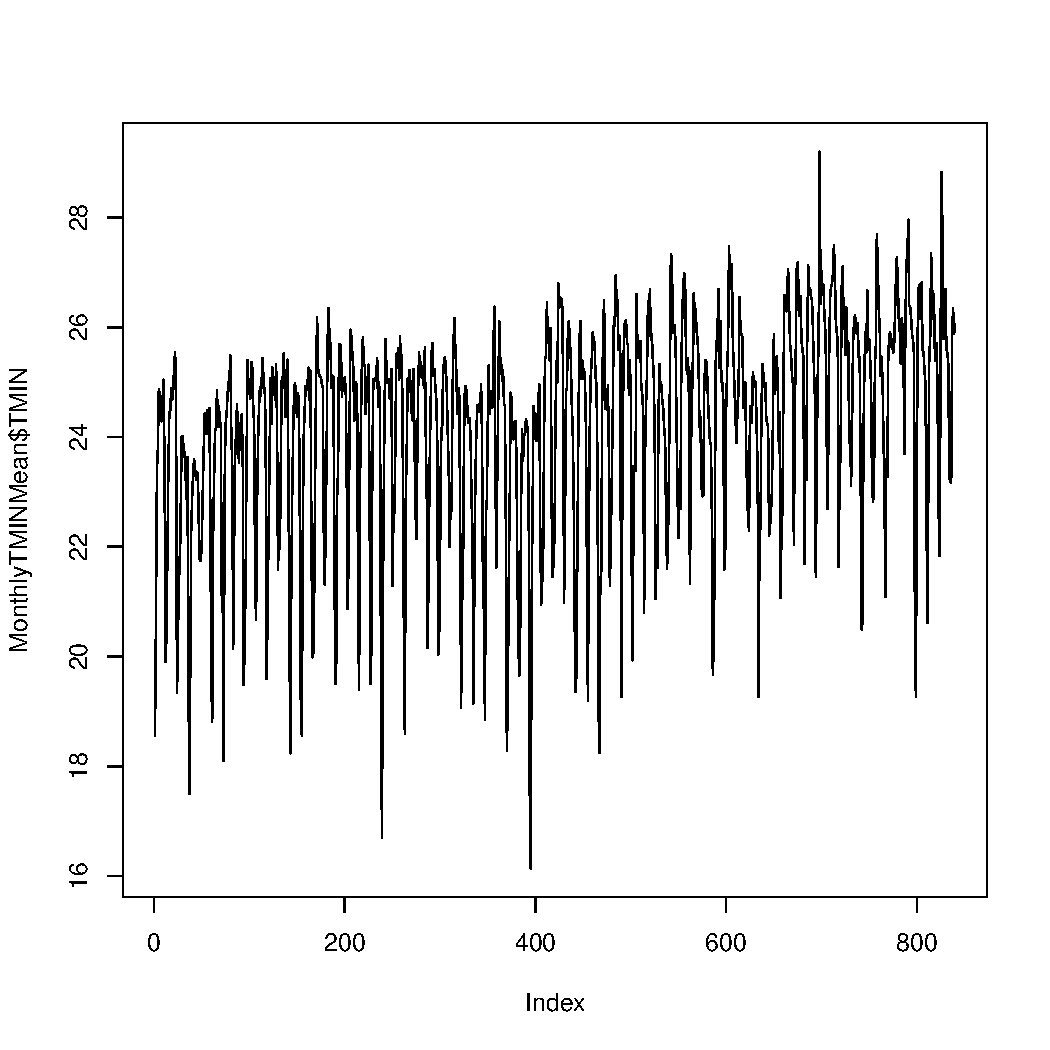
\includegraphics[width=\maxwidth]{figure/unnamed-chunk-13-1} 
\begin{kframe}\begin{alltt}
   \hlcom{#ylab("Number of Extreme Temps") + # for the y axis label}
\end{alltt}
\end{kframe}
\end{knitrout}

Rainfall...

\begin{knitrout}
\definecolor{shadecolor}{rgb}{0.969, 0.969, 0.969}\color{fgcolor}\begin{kframe}
\begin{alltt}
\hlkwd{ggplot}\hlstd{( )} \hlopt{+}
   \hlkwd{geom_bar}\hlstd{(}\hlkwc{data} \hlstd{= PRCP.Season.Total,}
      \hlkwd{aes}\hlstd{(}\hlkwc{x}\hlstd{=Year,} \hlkwc{y}\hlstd{=PRCP,} \hlkwc{fill}\hlstd{=Season),} \hlkwc{stat}\hlstd{=}\hlstr{"identity"}\hlstd{)} \hlopt{+}
         \hlkwd{xlim}\hlstd{(}\hlkwd{min}\hlstd{(CHCND}\hlopt{$}\hlstd{Year),} \hlkwd{max}\hlstd{(CHCND}\hlopt{$}\hlstd{Year)}\hlopt{-}\hlnum{1}\hlstd{)} \hlopt{+}
   \hlcom{#ylab("Number of Extreme Temps") + # for the y axis label}
   \hlkwd{geom_smooth}\hlstd{(}\hlkwc{data} \hlstd{= PRCP.Total,}
      \hlkwd{aes}\hlstd{(}\hlkwc{y}\hlstd{=PRCP,} \hlkwc{x}\hlstd{=Year),} \hlkwc{method} \hlstd{=} \hlstr{"lm"}\hlstd{,}
      \hlkwc{se} \hlstd{= T,} \hlkwc{color}\hlstd{=} \hlstr{"black"}\hlstd{)}
\end{alltt}


{\ttfamily\noindent\itshape\color{messagecolor}{\#\# `geom\_smooth()` using formula 'y \textasciitilde{} x'}}\end{kframe}
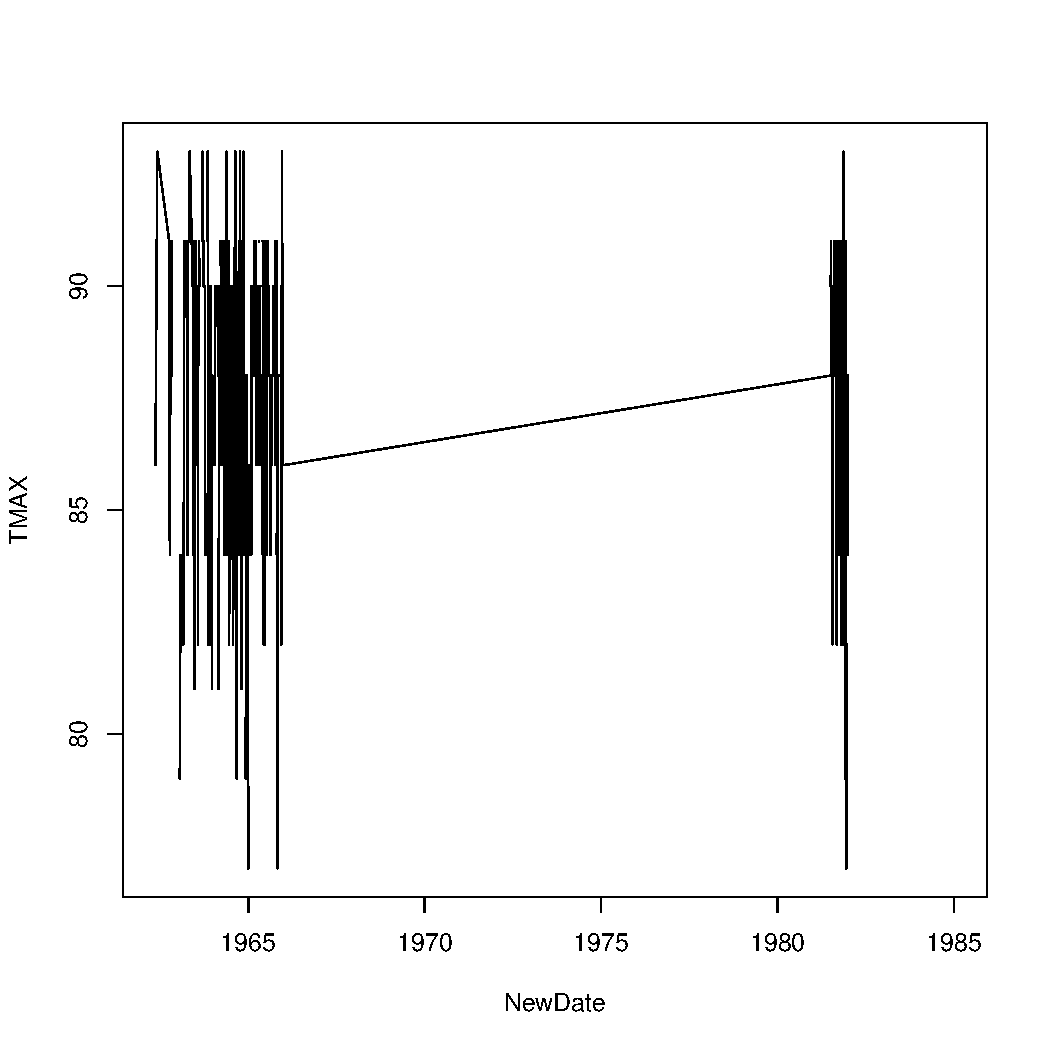
\includegraphics[width=\maxwidth]{figure/unnamed-chunk-14-1} 
\begin{kframe}\begin{alltt}
\hlcom{# + geom_smooth(data= PRCP.Season.Total, aes(x=Year, y = PRCP, color = Season, group=Season), se=F)}
\end{alltt}
\end{kframe}
\end{knitrout}

Days without rain...within a calendar year... bleed over between years isn't captured..

\begin{knitrout}
\definecolor{shadecolor}{rgb}{0.969, 0.969, 0.969}\color{fgcolor}\begin{kframe}
\begin{alltt}
\hlstd{CHCND}\hlopt{$}\hlstd{PRCP.count} \hlkwb{=} \hlkwd{sequence}\hlstd{(}\hlkwd{rle}\hlstd{(CHCND}\hlopt{$}\hlstd{PRCP)}\hlopt{$}\hlstd{lengths)}
\hlstd{Drought.run.temp} \hlkwb{<-} \hlkwd{data.frame}\hlstd{(}\hlkwc{Year} \hlstd{=} \hlnum{NA}\hlstd{,} \hlkwc{lengths}\hlstd{=}\hlnum{NA}\hlstd{,} \hlkwc{values}\hlstd{=}\hlnum{NA}\hlstd{)}
\hlkwa{for}\hlstd{(i} \hlkwa{in} \hlkwd{min}\hlstd{(CHCND}\hlopt{$}\hlstd{Year)}\hlopt{:}\hlkwd{max}\hlstd{(CHCND}\hlopt{$}\hlstd{Year))\{}
   \hlcom{# print(i)}
   \hlstd{run.length} \hlkwb{=} \hlkwd{rle}\hlstd{(CHCND[CHCND}\hlopt{$}\hlstd{Year}\hlopt{==}\hlstd{i,]}\hlopt{$}\hlstd{PRCP)}
   \hlstd{run.length.df} \hlkwb{=} \hlkwd{data.frame}\hlstd{(}\hlkwc{Year} \hlstd{=} \hlkwd{rep}\hlstd{(i,} \hlkwd{length}\hlstd{(run.length}\hlopt{$}\hlstd{values)),}
         \hlkwc{lengths} \hlstd{= run.length}\hlopt{$}\hlstd{lengths,}
         \hlkwc{values} \hlstd{= run.length}\hlopt{$}\hlstd{values)}

   \hlstd{Drought.run.temp} \hlkwb{<-} \hlkwd{rbind}\hlstd{(Drought.run.temp,}
         \hlstd{run.length.df[run.length.df}\hlopt{$}\hlstd{values}\hlopt{==}\hlnum{0}\hlstd{,])}
\hlstd{\}}
\hlstd{Drought.run} \hlkwb{<-} \hlstd{Drought.run.temp[}\hlopt{-}\hlnum{1}\hlstd{,]}
\hlkwd{str}\hlstd{(Drought.run)}
\end{alltt}
\begin{verbatim}
## 'data.frame':	7732 obs. of  3 variables:
##  $ Year   : int  NA NA NA NA NA NA NA NA NA NA ...
##  $ lengths: int  NA NA NA NA NA NA NA NA NA NA ...
##  $ values : int  NA NA NA NA NA NA NA NA NA NA ...
\end{verbatim}
\begin{alltt}
\hlkwd{names}\hlstd{(Drought.run)}
\end{alltt}
\begin{verbatim}
## [1] "Year"    "lengths" "values"
\end{verbatim}
\begin{alltt}
\hlcom{# What is a drought 10 days, 20 days, 40 days?}

\hlstd{Drought.run.10} \hlkwb{=} \hlkwd{aggregate}\hlstd{(lengths}\hlopt{~}\hlstd{Year,}
   \hlkwc{data}\hlstd{=Drought.run[Drought.run}\hlopt{$}\hlstd{lengths}\hlopt{>=}\hlnum{10}\hlstd{,], sum)}
\hlstd{Drought.run.20} \hlkwb{=} \hlkwd{aggregate}\hlstd{(lengths}\hlopt{~}\hlstd{Year,}
   \hlkwc{data}\hlstd{=Drought.run[Drought.run}\hlopt{$}\hlstd{lengths}\hlopt{>=}\hlnum{20}\hlstd{,], sum)}
\hlstd{Drought.run.40} \hlkwb{=} \hlkwd{aggregate}\hlstd{(lengths}\hlopt{~}\hlstd{Year,}
   \hlkwc{data}\hlstd{=Drought.run[Drought.run}\hlopt{$}\hlstd{lengths}\hlopt{>=}\hlnum{40}\hlstd{,], sum)}
\hlstd{Drought.run.100} \hlkwb{=} \hlkwd{aggregate}\hlstd{(lengths}\hlopt{~}\hlstd{Year,}
   \hlkwc{data}\hlstd{=Drought.run[Drought.run}\hlopt{$}\hlstd{lengths}\hlopt{>=}\hlnum{100}\hlstd{,], sum)}
\end{alltt}


{\ttfamily\noindent\bfseries\color{errorcolor}{\#\# Error in aggregate.data.frame(mf[1L], mf[-1L], FUN = FUN, ...): no rows to aggregate}}\begin{alltt}
\hlkwd{plot}\hlstd{(lengths}\hlopt{~}\hlstd{Year, Drought.run.10,} \hlkwc{pch}\hlstd{=}\hlnum{20}\hlstd{,} \hlkwc{cex}\hlstd{=}\hlnum{.5}\hlstd{)}
\hlkwd{points}\hlstd{(lengths}\hlopt{~}\hlstd{Year, Drought.run.20,} \hlkwc{pch}\hlstd{=}\hlnum{20}\hlstd{,} \hlkwc{col}\hlstd{=}\hlstr{"blue"}\hlstd{,} \hlkwc{cex}\hlstd{=}\hlnum{.5}\hlstd{)}
\hlkwd{points}\hlstd{(lengths}\hlopt{~}\hlstd{Year, Drought.run.40,} \hlkwc{pch}\hlstd{=}\hlnum{20}\hlstd{,} \hlkwc{col}\hlstd{=}\hlstr{"red"}\hlstd{,} \hlkwc{cex}\hlstd{=}\hlnum{.5}\hlstd{)}
\hlkwd{points}\hlstd{(lengths}\hlopt{~}\hlstd{Year, Drought.run.100,} \hlkwc{pch}\hlstd{=}\hlnum{20}\hlstd{,} \hlkwc{col}\hlstd{=}\hlstr{"purple"}\hlstd{,} \hlkwc{cex}\hlstd{=}\hlnum{.5}\hlstd{)}
\end{alltt}


{\ttfamily\noindent\bfseries\color{errorcolor}{\#\# Error in eval(m\$data, eframe): object 'Drought.run.100' not found}}\begin{alltt}
\hlkwd{abline}\hlstd{(}\hlkwd{lm}\hlstd{(lengths}\hlopt{~}\hlstd{Year, Drought.run.10))}
\hlkwd{abline}\hlstd{(}\hlkwd{lm}\hlstd{(lengths}\hlopt{~}\hlstd{Year, Drought.run.20),} \hlkwc{col}\hlstd{=}\hlstr{"blue"}\hlstd{)}
\hlkwd{abline}\hlstd{(}\hlkwd{lm}\hlstd{(lengths}\hlopt{~}\hlstd{Year, Drought.run.40),} \hlkwc{col}\hlstd{=}\hlstr{"red"}\hlstd{)}
\end{alltt}
\end{kframe}
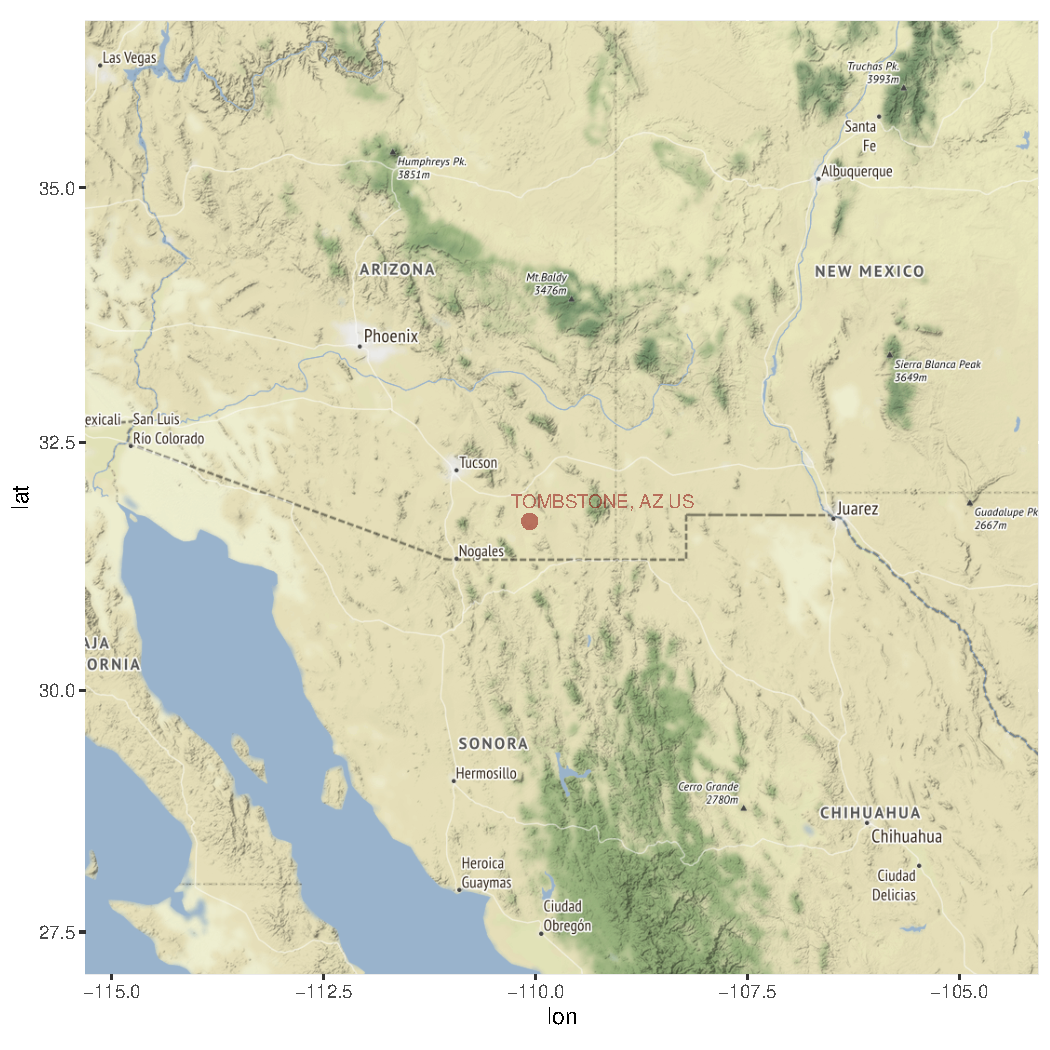
\includegraphics[width=\maxwidth]{figure/unnamed-chunk-15-1} 
\begin{kframe}\begin{alltt}
\hlkwd{abline}\hlstd{(}\hlkwd{lm}\hlstd{(lengths}\hlopt{~}\hlstd{Year, Drought.run.100),} \hlkwc{col}\hlstd{=}\hlstr{"purple"}\hlstd{)}
\end{alltt}


{\ttfamily\noindent\bfseries\color{errorcolor}{\#\# Error in is.data.frame(data): object 'Drought.run.100' not found}}\begin{alltt}
\hlkwd{summary}\hlstd{(}\hlkwd{lm}\hlstd{(lengths}\hlopt{~}\hlstd{Year, Drought.run.100))}
\end{alltt}


{\ttfamily\noindent\bfseries\color{errorcolor}{\#\# Error in is.data.frame(data): object 'Drought.run.100' not found}}\begin{alltt}
\hlkwd{plot}\hlstd{(lengths}\hlopt{~}\hlstd{Year, Drought.run[Drought.run}\hlopt{$}\hlstd{lengths}\hlopt{>}\hlnum{30}\hlstd{,],} \hlkwc{pch}\hlstd{=}\hlnum{20}\hlstd{)}
\hlkwd{plot}\hlstd{(lengths}\hlopt{~}\hlstd{Year, Drought.run[Drought.run}\hlopt{$}\hlstd{lengths}\hlopt{>}\hlnum{30}\hlstd{,],} \hlkwc{pch}\hlstd{=}\hlnum{20}\hlstd{)}


\hlstd{Drought.run.lm} \hlkwb{<-} \hlkwd{lm}\hlstd{(lengths}\hlopt{~}\hlstd{Year, Drought.run[Drought.run}\hlopt{$}\hlstd{lengths}\hlopt{>}\hlnum{10}\hlstd{,])}
\hlkwd{summary}\hlstd{(Drought.run.lm)}
\end{alltt}
\begin{verbatim}
## 
## Call:
## lm(formula = lengths ~ Year, data = Drought.run[Drought.run$lengths > 
##     10, ])
## 
## Residuals:
##    Min     1Q Median     3Q    Max 
## -5.095 -3.585 -1.699  1.715 47.269 
## 
## Coefficients:
##              Estimate Std. Error t value Pr(>|t|)   
## (Intercept) 38.231403  11.717890   3.263  0.00117 **
## Year        -0.011657   0.005984  -1.948  0.05189 . 
## ---
## Signif. codes:  
## 0 '***' 0.001 '**' 0.01 '*' 0.05 '.' 0.1 ' ' 1
## 
## Residual standard error: 5.257 on 598 degrees of freedom
##   (954 observations deleted due to missingness)
## Multiple R-squared:  0.006305,	Adjusted R-squared:  0.004643 
## F-statistic: 3.794 on 1 and 598 DF,  p-value: 0.05189
\end{verbatim}
\begin{alltt}
\hlkwd{text}\hlstd{(}\hlkwd{min}\hlstd{(Drought.run}\hlopt{$}\hlstd{Year,} \hlkwc{na.rm}\hlstd{=T),} \hlkwd{max}\hlstd{(Drought.run}\hlopt{$}\hlstd{lengths,} \hlkwc{na.rm}\hlstd{=T),}
     \hlkwd{paste}\hlstd{(}\hlstr{"Slope (x100) = "}\hlstd{,} \hlkwd{round}\hlstd{(}\hlkwd{coef}\hlstd{(Drought.run.lm)[}\hlnum{2}\hlstd{]}\hlopt{*}\hlnum{100}\hlstd{,} \hlnum{3}\hlstd{)),} \hlkwc{pos}\hlstd{=}\hlnum{4}\hlstd{)}
\end{alltt}
\end{kframe}
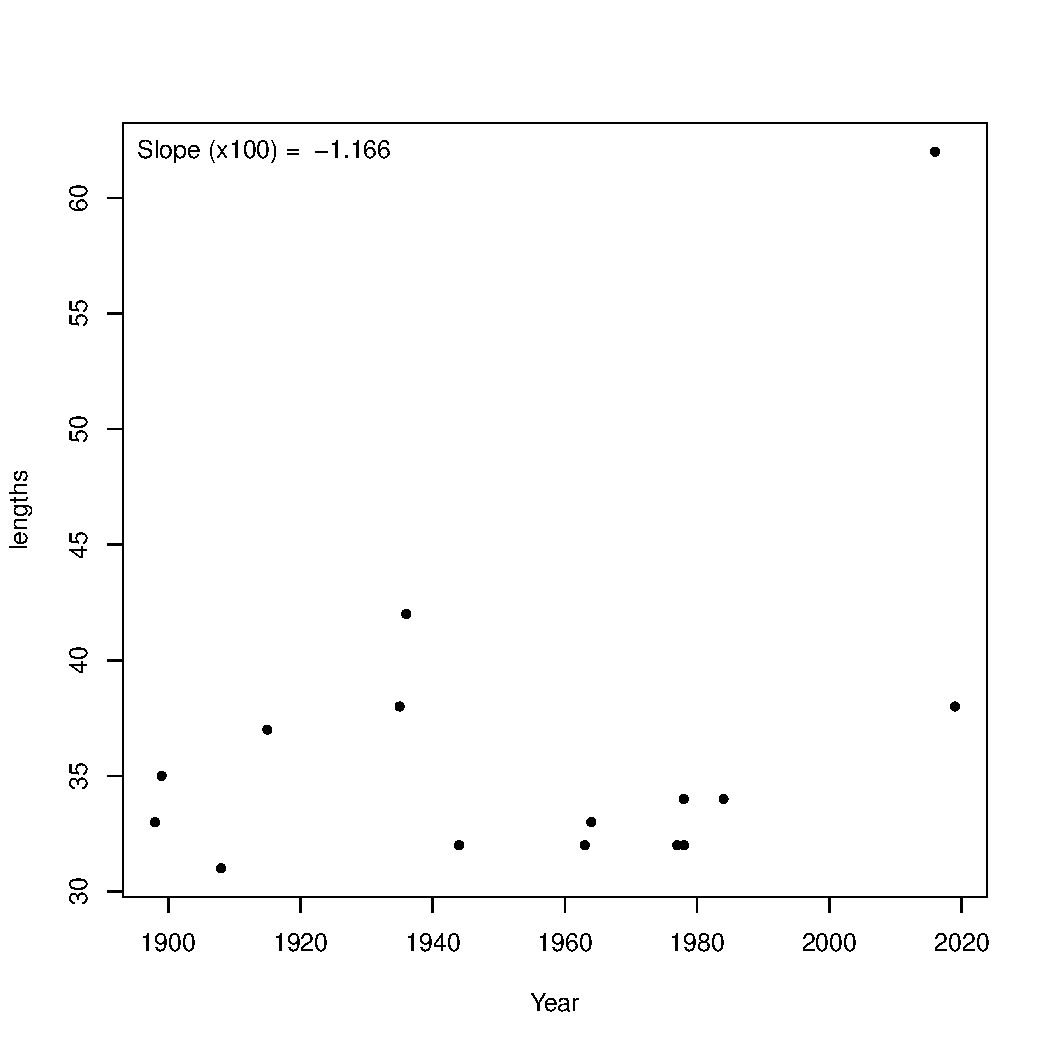
\includegraphics[width=\maxwidth]{figure/unnamed-chunk-15-2} 
\begin{kframe}\begin{alltt}
\hlcom{#plot(PRCP.count ~ Year, data=CHCND[CHCND$PRCP==0,])}
\end{alltt}
\end{kframe}
\end{knitrout}

Probability Distributions by decade...

\begin{knitrout}
\definecolor{shadecolor}{rgb}{0.969, 0.969, 0.969}\color{fgcolor}\begin{kframe}
\begin{alltt}
\hlstd{CHCND}\hlopt{$}\hlstd{Decade} \hlkwb{<-} \hlkwd{floor_decade}\hlstd{(CHCND}\hlopt{$}\hlstd{Year)}

\hlstd{PRCP.Decade} \hlkwb{<-} \hlkwd{aggregate}\hlstd{(PRCP}\hlopt{~}\hlstd{Month}\hlopt{+}\hlstd{Decade,} \hlkwc{data}\hlstd{=CHCND, sum)}
\hlkwd{head}\hlstd{(PRCP.Decade)}
\end{alltt}
\begin{verbatim}
##   Month Decade PRCP
## 1     1   1890 1504
## 2     2   1890 1772
## 3     3   1890 4060
## 4     4   1890 2966
## 5     5   1890  982
## 6     6   1890 2044
\end{verbatim}
\begin{alltt}
\hlstd{x} \hlkwb{<-} \hlstd{PRCP.Decade}\hlopt{$}\hlstd{PRCP[PRCP.Decade}\hlopt{$}\hlstd{Decade}\hlopt{==}\hlnum{1900}\hlstd{]}
\hlstd{df} \hlkwb{<-} \hlkwd{approxfun}\hlstd{(}\hlkwd{density}\hlstd{(x))}
\hlkwd{plot}\hlstd{(}\hlnum{1}\hlopt{:}\hlnum{12}\hlstd{,} \hlkwd{density}\hlstd{(x))}
\end{alltt}


{\ttfamily\noindent\bfseries\color{errorcolor}{\#\# Error in xy.coords(x, y, xlabel, ylabel, log): 'x' and 'y' lengths differ}}\begin{alltt}
\hlstd{xnew} \hlkwb{<-} \hlkwd{c}\hlstd{(}\hlnum{0.45}\hlstd{,}\hlnum{1.84}\hlstd{,}\hlnum{2.3}\hlstd{)}
\hlkwd{points}\hlstd{(xnew,}\hlkwd{df}\hlstd{(xnew),}\hlkwc{col}\hlstd{=}\hlnum{2}\hlstd{)}
\end{alltt}


{\ttfamily\noindent\bfseries\color{errorcolor}{\#\# Error in plot.xy(xy.coords(x, y), type = type, ...): plot.new has not been called yet}}\end{kframe}
\end{knitrout}

\begin{knitrout}
\definecolor{shadecolor}{rgb}{0.969, 0.969, 0.969}\color{fgcolor}\begin{kframe}
\begin{alltt}
\hlstd{CHCND}\hlopt{$}\hlstd{Score} \hlkwb{<-} \hlkwd{floor_score}\hlstd{(CHCND}\hlopt{$}\hlstd{Year)}
\end{alltt}
\end{kframe}
\end{knitrout}

\subsection{Determine Record Setting Temperatures}

In many cases, people seem to "feel" how temperature has been changing over time, and new records seem to capture the attention in the media. So, we'll create a updated record of maximum temperatures and display them. 



Crating a graphic of the results...


\subsubsection{Number of Days with Records per year}

This is a common way to communicate temperatures changes. I suspect we have a better sense of change when we notice "extreme" events...

\begin{knitrout}
\definecolor{shadecolor}{rgb}{0.969, 0.969, 0.969}\color{fgcolor}\begin{kframe}
\begin{alltt}
\hlkwd{names}\hlstd{(CHCND)}
\end{alltt}
\begin{verbatim}
##  [1] "DATE"       "TMAX"       "TMIN"       "PRCP"      
##  [5] "Date"       "Month"      "Month.name" "Year"      
##  [9] "YearDay"    "Season"     "PRCP.count" "Decade"    
## [13] "Score"      "mmdd"       "minTMIN"    "maxTMAX"
\end{verbatim}
\begin{alltt}
\hlstd{minTMIN.length} \hlkwb{=} \hlkwd{aggregate}\hlstd{(minTMIN}\hlopt{~}\hlstd{Year,} \hlkwc{data}\hlstd{=CHCND, length)}
\hlstd{minTMIN.length}\hlopt{$}\hlstd{group} \hlkwb{<-} \hlstr{"Record Lows"}
\hlkwd{names}\hlstd{(minTMIN.length)} \hlkwb{<-} \hlkwd{c}\hlstd{(}\hlstr{"Year"}\hlstd{,} \hlstr{"Num"}\hlstd{,} \hlstr{"Group"}\hlstd{)}
\hlstd{minTMIN.length}\hlopt{$}\hlstd{Num} \hlkwb{=} \hlopt{-}\hlstd{minTMIN.length}\hlopt{$}\hlstd{Num}

\hlstd{maxTMAX.length} \hlkwb{=} \hlkwd{aggregate}\hlstd{(maxTMAX}\hlopt{~}\hlstd{Year,} \hlkwc{data}\hlstd{=CHCND, length);}
\hlstd{maxTMAX.length}\hlopt{$}\hlstd{group} \hlkwb{<-} \hlstr{"Record Highs"}
\hlkwd{names}\hlstd{(maxTMAX.length)} \hlkwb{<-} \hlkwd{c}\hlstd{(}\hlstr{"Year"}\hlstd{,} \hlstr{"Num"}\hlstd{,} \hlstr{"Group"}\hlstd{)}

\hlstd{records} \hlkwb{=} \hlkwd{rbind}\hlstd{(minTMIN.length, maxTMAX.length);} \hlcom{# records}


\hlkwd{ggplot}\hlstd{( )} \hlopt{+}
   \hlkwd{geom_point}\hlstd{(}\hlkwc{data} \hlstd{= CHCND,} \hlkwd{aes}\hlstd{(}\hlkwc{y}\hlstd{=TMIN,} \hlkwc{x}\hlstd{=YearDay),}
      \hlkwc{size}\hlstd{=}\hlnum{.05}\hlstd{,} \hlkwc{color}\hlstd{=}\hlstr{"gray"}\hlstd{)} \hlopt{+}
   \hlkwd{geom_bar}\hlstd{(}\hlkwc{data} \hlstd{= records,} \hlkwd{aes}\hlstd{(}\hlkwc{x}\hlstd{=Year,} \hlkwc{y}\hlstd{=Num,} \hlkwc{fill}\hlstd{=Group),}
      \hlkwc{stat}\hlstd{=}\hlstr{"identity"}\hlstd{,} \hlkwc{position}\hlstd{=}\hlstr{"identity"}\hlstd{)} \hlopt{+}
   \hlkwd{xlim}\hlstd{(}\hlkwd{min}\hlstd{(CHCND}\hlopt{$}\hlstd{Year),} \hlkwd{max}\hlstd{(CHCND}\hlopt{$}\hlstd{Year)}\hlopt{-}\hlnum{1}\hlstd{)} \hlopt{+}
   \hlcom{#ylab("Number of Extreme Temps") + # for the y axis label}
   \hlkwd{scale_fill_manual}\hlstd{(}\hlstr{"Legend"}\hlstd{,}
      \hlkwc{values} \hlstd{=} \hlkwd{c}\hlstd{(}\hlstr{"Record Highs"} \hlstd{=} \hlstr{"red"}\hlstd{,} \hlstr{"Record Lows"} \hlstd{=} \hlstr{"blue"}\hlstd{))} \hlopt{+}
   \hlkwd{geom_smooth}\hlstd{(}\hlkwc{data} \hlstd{= CHCND,} \hlkwd{aes}\hlstd{(}\hlkwc{y}\hlstd{=TMIN,} \hlkwc{x}\hlstd{=YearDay),} \hlkwc{method} \hlstd{=} \hlstr{"lm"}\hlstd{,} \hlkwc{se} \hlstd{=} \hlnum{FALSE}\hlstd{)}
\end{alltt}


{\ttfamily\noindent\itshape\color{messagecolor}{\#\# `geom\_smooth()` using formula 'y \textasciitilde{} x'}}

{\ttfamily\noindent\color{warningcolor}{\#\# Warning: Removed 878 rows containing non-finite values\\\#\# (stat\_smooth).}}

{\ttfamily\noindent\color{warningcolor}{\#\# Warning: Removed 878 rows containing missing values (geom\_point).}}

{\ttfamily\noindent\color{warningcolor}{\#\# Warning: Removed 3 rows containing missing values (geom\_bar).}}\end{kframe}
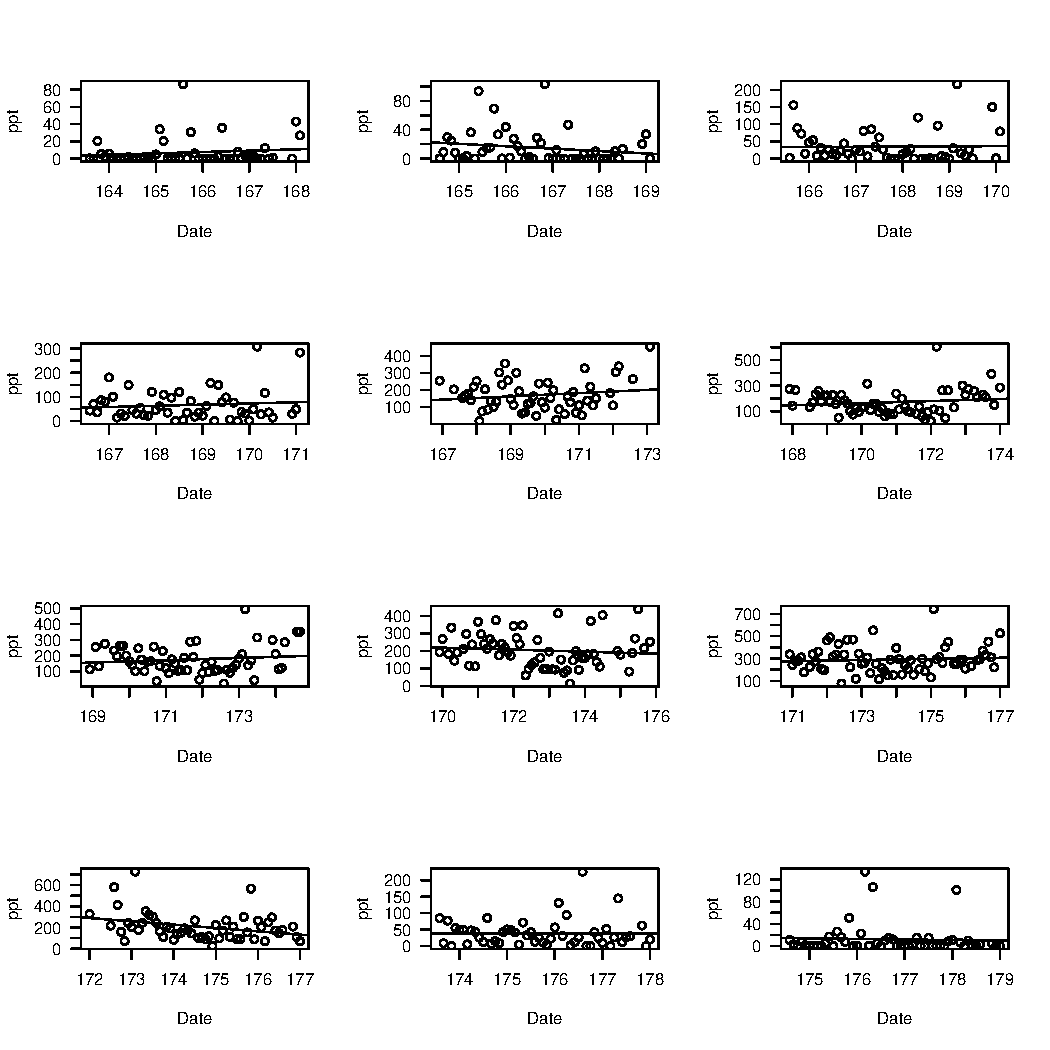
\includegraphics[width=\maxwidth]{figure/unnamed-chunk-18-1} 
\begin{kframe}\begin{alltt}
\hlcom{#scale_y_continuous(}
    \hlcom{# Features of the first axis}
    \hlcom{# name = "Temperature (F °)",}
    \hlcom{# Add a second axis and specify its features}
    \hlcom{# sec.axis = sec_axis(~.*Num, name="Number of Extreme Temps")}
  \hlcom{#) }
\end{alltt}
\end{kframe}
\end{knitrout}

\subsection{Iterate TMAX vs. Month Boxplots}



\section{Static Plot Results}

\subsection{Four Plots}

To test the code, I have created graphics that can then be used in the animation process, i.e. try to create code that doesn't get too complicated and then fail! 

\begin{knitrout}
\definecolor{shadecolor}{rgb}{0.969, 0.969, 0.969}\color{fgcolor}\begin{kframe}
\begin{verbatim}
## pdf 
##   2
\end{verbatim}
\end{kframe}
\end{knitrout}

\begin{figure}
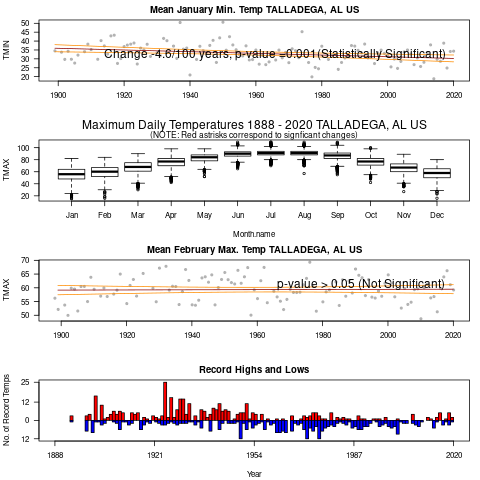
\includegraphics[width=1.00\textwidth]{/home/CAMPUS/mwl04747/github/Climate_Change_Narratives/Social_Media/png/Alabama-USC00018024-GSOM.png}
\caption{Climate can be analyzed using several types of lenses. In this case, we have analyzed show the months with the greatest changes. The first figure is monthly average of TMINs (daily low temperatures) with a best fit line. The second figure shows the monthly TMAX range and asterisks indicate singificant changes over the station record and the third figure is the trend for these TMAXs over time and includes the best fit line. The final figure shows the daily temperatures that have been the highest on record (in red). In some cases, climate change has created more records in the recent decades, while other stations seem don't show that trend.}
\label{fig:GSOM}
\end{figure}

\subsection{KISS}

Keeping it simple is critical in communicating scientific information. In this section, I try to come up with a consistent message for every state and a simple graphic. 

First, TMIN and TMAX and change point analysis...

https://cran.r-project.org/web/packages/mcp/readme/README.html

\begin{knitrout}
\definecolor{shadecolor}{rgb}{0.969, 0.969, 0.969}\color{fgcolor}\begin{kframe}
\begin{alltt}
\hlkwd{library}\hlstd{(mcp)}
\hlkwd{library}\hlstd{(rlang)}

\hlcom{# Simulate}
\hlkwd{set.seed}\hlstd{(}\hlnum{42}\hlstd{)}  \hlcom{# I always use 42; no fiddling}
\hlstd{df} \hlkwb{=} \hlkwd{data.frame}\hlstd{(}
  \hlkwc{x} \hlstd{=} \hlnum{1}\hlopt{:}\hlnum{100}\hlstd{,}
  \hlkwc{y} \hlstd{=} \hlkwd{c}\hlstd{(}\hlkwd{rnorm}\hlstd{(}\hlnum{30}\hlstd{,} \hlnum{2}\hlstd{),} \hlkwd{rnorm}\hlstd{(}\hlnum{40}\hlstd{,} \hlnum{0}\hlstd{),} \hlkwd{rnorm}\hlstd{(}\hlnum{30}\hlstd{,} \hlnum{1}\hlstd{))}
\hlstd{)}

\hlcom{# Plot it}
\hlkwd{plot}\hlstd{(df)}
\hlkwd{abline}\hlstd{(}\hlkwc{v} \hlstd{=} \hlkwd{c}\hlstd{(}\hlnum{30}\hlstd{,} \hlnum{70}\hlstd{),} \hlkwc{col}\hlstd{=}\hlstr{"red"}\hlstd{)}

\hlstd{model} \hlkwb{=} \hlkwd{list}\hlstd{(y}\hlopt{~}\hlnum{1}\hlstd{,} \hlnum{1}\hlopt{~}\hlnum{1}\hlstd{,} \hlnum{1}\hlopt{~}\hlnum{1}\hlstd{)}  \hlcom{# three intercept-only segments}
\hlstd{fit_mcp} \hlkwb{=} \hlkwd{mcp}\hlstd{(model,} \hlkwc{data} \hlstd{= df,} \hlkwc{par_x} \hlstd{=} \hlstr{"x"}\hlstd{)}

\hlkwd{summary}\hlstd{(fit_mcp)}

\hlkwd{library}\hlstd{(patchwork)}
\hlkwd{plot}\hlstd{(fit_mcp)} \hlopt{+} \hlkwd{plot_pars}\hlstd{(fit_mcp,} \hlkwc{pars} \hlstd{=} \hlkwd{c}\hlstd{(}\hlstr{"cp_1"}\hlstd{,} \hlstr{"cp_2"}\hlstd{),} \hlkwc{type} \hlstd{=} \hlstr{"dens_overlay"}\hlstd{)}

\hlstd{model} \hlkwb{=} \hlkwd{list}\hlstd{(}
  \hlstd{price} \hlopt{~} \hlnum{1} \hlopt{+} \hlkwd{ar}\hlstd{(}\hlnum{2}\hlstd{),}
  \hlopt{~} \hlnum{0} \hlopt{+} \hlstd{time} \hlopt{+} \hlkwd{ar}\hlstd{(}\hlnum{1}\hlstd{)}
\hlstd{)}
\hlstd{ex} \hlkwb{=} \hlkwd{mcp_example}\hlstd{(}\hlstr{"ar"}\hlstd{)}
\hlstd{fit} \hlkwb{=} \hlkwd{mcp}\hlstd{(model, ex}\hlopt{$}\hlstd{data)}
\hlkwd{summary}\hlstd{(fit)}
\end{alltt}
\end{kframe}
\end{knitrout}

Let's create a figure that simplifies the narrative, if we can!

\begin{knitrout}
\definecolor{shadecolor}{rgb}{0.969, 0.969, 0.969}\color{fgcolor}\begin{kframe}
\begin{verbatim}
## pdf 
##   2
\end{verbatim}
\end{kframe}
\end{knitrout}

\begin{figure}
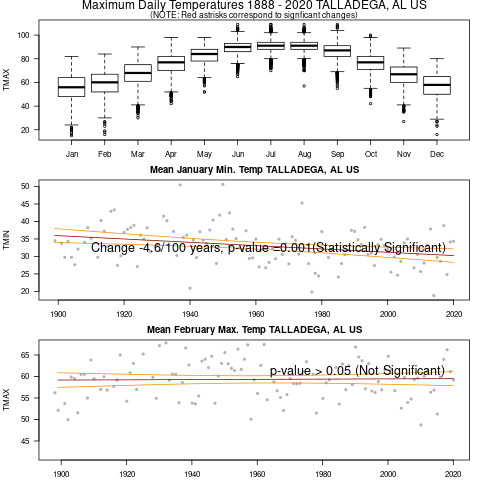
\includegraphics[width=1.00\textwidth]{/home/CAMPUS/mwl04747/github/Climate_Change_Narratives/Social_Media/png/Alabama-USC00018024-KISS.png}
\caption{Keep it simple stupid!}
\label{fig:GSOM-KISS}
\end{figure}



\subsection{Temp \& Precipitation Probability}

To highlight the patterns of change, it might be useful to analyze how the probability ditributuion might change -- we can use a normal probability distribion as a theoretical distribution (and we can check if this distribuion is approrpriate with a Chi-Square test), or we can use the data to create a emperical distribution, which is my favored approach. 

I started with decade bins, but used 20 years bins (scores) to simplify the graphics while keeping a pretty good temporal resolution.

\begin{knitrout}
\definecolor{shadecolor}{rgb}{0.969, 0.969, 0.969}\color{fgcolor}\begin{kframe}
\begin{alltt}
\hlkwd{library}\hlstd{(wesanderson)}

\hlstd{h.ramp} \hlkwb{<-} \hlkwd{rev}\hlstd{(}\hlkwd{heat.colors}\hlstd{(}\hlkwd{length}\hlstd{(}\hlkwd{unique}\hlstd{(GSOM2}\hlopt{$}\hlstd{Score))}\hlopt{+}\hlnum{1}\hlstd{))[}\hlopt{-}\hlnum{1}\hlstd{]}
\hlstd{h.ramp} \hlkwb{<-} \hlkwd{wes_palette}\hlstd{(}\hlstr{"Zissou1"}\hlstd{,} \hlkwd{length}\hlstd{(}\hlkwd{unique}\hlstd{(GSOM2}\hlopt{$}\hlstd{Score)),}
      \hlkwc{type} \hlstd{=} \hlstr{"continuous"}\hlstd{)[}\hlnum{1}\hlopt{:}\hlkwd{length}\hlstd{(}\hlkwd{unique}\hlstd{(GSOM2}\hlopt{$}\hlstd{Score))]}
\hlcom{#TMAX.anomaly.Score = aggregate(TMAX.anom ~ Score, GSOM2, mean)}
\hlcom{#TMAX.sd.anomaly.Score = aggregate(TMAX.anom ~ Score, GSOM2, sd)}


\hlcom{# I hate list!}
\hlstd{TMAX.anomaly.list} \hlkwb{=} \hlkwd{aggregate}\hlstd{(TMAX.anom} \hlopt{~} \hlstd{Score, GSOM2,}
   \hlkwc{FUN} \hlstd{=} \hlkwa{function}\hlstd{(}\hlkwc{x}\hlstd{)} \hlkwd{c}\hlstd{(}\hlkwc{mean} \hlstd{=} \hlkwd{mean}\hlstd{(x),} \hlkwc{sd} \hlstd{=} \hlkwd{sd}\hlstd{(x)))}
\hlstd{TMIN.anomaly.list} \hlkwb{=} \hlkwd{aggregate}\hlstd{(TMIN.anom} \hlopt{~} \hlstd{Score, GSOM2,}
   \hlkwc{FUN} \hlstd{=} \hlkwa{function}\hlstd{(}\hlkwc{x}\hlstd{)} \hlkwd{c}\hlstd{(}\hlkwc{mean} \hlstd{=} \hlkwd{mean}\hlstd{(x),} \hlkwc{sd} \hlstd{=} \hlkwd{sd}\hlstd{(x)))}
\hlstd{PPT.anomaly.list} \hlkwb{=} \hlkwd{aggregate}\hlstd{(PPT.anom} \hlopt{~} \hlstd{Score, GSOM2,}
   \hlkwc{FUN} \hlstd{=} \hlkwa{function}\hlstd{(}\hlkwc{x}\hlstd{)} \hlkwd{c}\hlstd{(}\hlkwc{mean} \hlstd{=} \hlkwd{mean}\hlstd{(x),} \hlkwc{sd} \hlstd{=} \hlkwd{sd}\hlstd{(x)))}


\hlkwd{setwd}\hlstd{(}\hlstr{"/home/CAMPUS/mwl04747/github/Climate_Change_Narratives/Social_Media"}\hlstd{)}
\hlkwd{png}\hlstd{(}\hlkwd{paste0}\hlstd{(}\hlstr{"png//"}\hlstd{, fips}\hlopt{$}\hlstd{State,} \hlstr{"-"}\hlstd{, stid,} \hlstr{"-GSOM-normalPDF.png"}\hlstd{),}
    \hlkwc{width} \hlstd{=} \hlnum{480}\hlstd{,} \hlkwc{height} \hlstd{=} \hlnum{480}\hlstd{,} \hlkwc{units} \hlstd{=} \hlstr{"px"}\hlstd{,} \hlkwc{pointsize} \hlstd{=} \hlnum{12}\hlstd{,} \hlkwc{bg} \hlstd{=} \hlstr{"white"}\hlstd{)}
\hlcom{# TMIN}
\hlkwd{par}\hlstd{(}\hlkwc{mfrow}\hlstd{=}\hlkwd{c}\hlstd{(}\hlnum{2}\hlstd{,}\hlnum{2}\hlstd{),} \hlkwc{las}\hlstd{=}\hlnum{1}\hlstd{)}
\hlstd{Anom.x} \hlkwb{=} \hlkwd{seq}\hlstd{(}\hlkwd{min}\hlstd{(GSOM2}\hlopt{$}\hlstd{TMIN.anom),} \hlkwd{max}\hlstd{(GSOM2}\hlopt{$}\hlstd{TMIN.anom),}\hlkwc{by}\hlstd{=}\hlnum{.1}\hlstd{)}
\hlstd{Anom.y} \hlkwb{=} \hlkwd{max}\hlstd{(}\hlkwd{dnorm}\hlstd{(Anom.x,}
   \hlkwc{mean}\hlstd{=TMIN.anomaly.list}\hlopt{$}\hlstd{TMIN.anom[}\hlnum{1}\hlstd{,}\hlnum{1}\hlstd{],}
   \hlkwc{sd}\hlstd{=TMIN.anomaly.list}\hlopt{$}\hlstd{TMIN.anom[}\hlnum{1}\hlstd{,}\hlnum{2}\hlstd{]))}\hlopt{*}\hlnum{1.2}

\hlkwd{plot}\hlstd{(Anom.x,} \hlkwd{dnorm}\hlstd{(Anom.x,}
   \hlkwc{mean}\hlstd{=TMIN.anomaly.list}\hlopt{$}\hlstd{TMIN.anom[}\hlnum{1}\hlstd{,} \hlnum{1}\hlstd{],}
   \hlkwc{sd}\hlstd{=TMIN.anomaly.list}\hlopt{$}\hlstd{TMIN.anom[}\hlnum{1}\hlstd{,} \hlnum{2}\hlstd{]),}
   \hlkwc{ty}\hlstd{=}\hlstr{"l"}\hlstd{,} \hlkwc{col}\hlstd{=h.ramp[}\hlnum{1}\hlstd{],} \hlkwc{ylim}\hlstd{=}\hlkwd{c}\hlstd{(}\hlnum{0}\hlstd{, Anom.y),}
   \hlkwc{ylab}\hlstd{=}\hlstr{"Density"}\hlstd{,} \hlkwc{xlab}\hlstd{=}\hlstr{"TMIN Anomaly (°F)"}\hlstd{,} \hlkwc{main}\hlstd{=}\hlstr{""}\hlstd{)}

\hlkwd{abline}\hlstd{(}\hlkwc{v}\hlstd{=TMIN.anomaly.list}\hlopt{$}\hlstd{TMIN.anom[}\hlnum{1}\hlstd{,}\hlnum{1}\hlstd{],} \hlkwc{col}\hlstd{=h.ramp[}\hlnum{1}\hlstd{],} \hlkwc{lwd}\hlstd{=}\hlnum{2}\hlstd{)}
\hlkwa{for}\hlstd{(i} \hlkwa{in} \hlnum{2}\hlopt{:}\hlkwd{nrow}\hlstd{(TMIN.anomaly.list))\{}
\hlkwd{lines}\hlstd{(Anom.x,} \hlkwd{dnorm}\hlstd{(Anom.x,}
   \hlkwc{mean}\hlstd{=TMIN.anomaly.list}\hlopt{$}\hlstd{TMIN.anom[i,} \hlnum{1}\hlstd{],}
   \hlkwc{sd}\hlstd{=TMIN.anomaly.list}\hlopt{$}\hlstd{TMIN.anom[i,} \hlnum{2}\hlstd{]),} \hlkwc{col}\hlstd{=h.ramp[i])}
\hlstd{\}}
\hlkwd{abline}\hlstd{(}\hlkwc{v}\hlstd{=TMIN.anomaly.list}\hlopt{$}\hlstd{TMIN.anom[i,}\hlnum{1}\hlstd{],} \hlkwc{col}\hlstd{=h.ramp[i],} \hlkwc{lwd}\hlstd{=}\hlnum{2}\hlstd{)}
\hlstd{Delta} \hlkwb{=} \hlstd{TMIN.anomaly.list}\hlopt{$}\hlstd{TMIN.anom[i,}\hlnum{1}\hlstd{]} \hlopt{-} \hlstd{TMIN.anomaly.list}\hlopt{$}\hlstd{TMIN.anom[}\hlnum{1}\hlstd{,}\hlnum{1}\hlstd{]}

\hlkwd{text}\hlstd{(TMIN.anomaly.list}\hlopt{$}\hlstd{TMIN.anom[i,}\hlnum{1}\hlstd{], Anom.y}\hlopt{*}\hlnum{.9}\hlstd{,}
   \hlkwd{paste0}\hlstd{(}\hlstr{"Change "}\hlstd{,} \hlkwd{round}\hlstd{(Delta,} \hlnum{1}\hlstd{),} \hlstr{"°F"}\hlstd{),} \hlkwc{pos}\hlstd{=}\hlnum{4}\hlstd{)}

\hlkwd{mtext}\hlstd{(}\hlkwd{paste0}\hlstd{(fips}\hlopt{$}\hlstd{State,} \hlstr{" ("}\hlstd{, GSOM_Longest}\hlopt{$}\hlstd{name,} \hlstr{")"}\hlstd{),} \hlkwc{side}\hlstd{=}\hlnum{3}\hlstd{,} \hlkwc{line}\hlstd{=}\hlnum{2}\hlstd{)}

\hlcom{# TMAX}
\hlstd{Anom.x} \hlkwb{=} \hlkwd{seq}\hlstd{(}\hlkwd{min}\hlstd{(GSOM2}\hlopt{$}\hlstd{TMAX.anom),} \hlkwd{max}\hlstd{(GSOM2}\hlopt{$}\hlstd{TMAX.anom),}\hlkwc{by}\hlstd{=}\hlnum{.1}\hlstd{)}
\hlstd{Anom.y} \hlkwb{=} \hlkwd{max}\hlstd{(}\hlkwd{dnorm}\hlstd{(Anom.x,}
   \hlkwc{mean}\hlstd{=TMAX.anomaly.list}\hlopt{$}\hlstd{TMAX.anom[}\hlnum{1}\hlstd{,}\hlnum{1}\hlstd{],}
   \hlkwc{sd}\hlstd{=TMAX.anomaly.list}\hlopt{$}\hlstd{TMAX.anom[}\hlnum{1}\hlstd{,}\hlnum{2}\hlstd{]))}\hlopt{*}\hlnum{1.2}

\hlkwd{plot}\hlstd{(Anom.x,} \hlkwd{dnorm}\hlstd{(Anom.x,}
   \hlkwc{mean}\hlstd{=TMAX.anomaly.list}\hlopt{$}\hlstd{TMAX.anom[}\hlnum{1}\hlstd{,} \hlnum{1}\hlstd{],}
   \hlkwc{sd}\hlstd{=TMAX.anomaly.list}\hlopt{$}\hlstd{TMAX.anom[}\hlnum{1}\hlstd{,} \hlnum{2}\hlstd{]),}
   \hlkwc{ty}\hlstd{=}\hlstr{"l"}\hlstd{,} \hlkwc{col}\hlstd{=h.ramp[}\hlnum{1}\hlstd{],} \hlkwc{ylim}\hlstd{=}\hlkwd{c}\hlstd{(}\hlnum{0}\hlstd{, Anom.y),}
   \hlkwc{ylab}\hlstd{=}\hlstr{"Density"}\hlstd{,} \hlkwc{xlab}\hlstd{=}\hlstr{"TMAX Anomaly (°F)"}\hlstd{)}

\hlkwd{abline}\hlstd{(}\hlkwc{v}\hlstd{=TMAX.anomaly.list}\hlopt{$}\hlstd{TMAX.anom[}\hlnum{1}\hlstd{,}\hlnum{1}\hlstd{],} \hlkwc{col}\hlstd{=h.ramp[}\hlnum{1}\hlstd{],} \hlkwc{lwd}\hlstd{=}\hlnum{2}\hlstd{)}
\hlkwa{for}\hlstd{(i} \hlkwa{in} \hlnum{2}\hlopt{:}\hlkwd{nrow}\hlstd{(TMAX.anomaly.list))\{}
\hlkwd{lines}\hlstd{(Anom.x,} \hlkwd{dnorm}\hlstd{(Anom.x,}
   \hlkwc{mean}\hlstd{=TMAX.anomaly.list}\hlopt{$}\hlstd{TMAX.anom[i,} \hlnum{1}\hlstd{],}
   \hlkwc{sd}\hlstd{=TMAX.anomaly.list}\hlopt{$}\hlstd{TMAX.anom[i,} \hlnum{2}\hlstd{]),} \hlkwc{col}\hlstd{=h.ramp[i])}
\hlstd{\}}
\hlkwd{abline}\hlstd{(}\hlkwc{v}\hlstd{=TMAX.anomaly.list}\hlopt{$}\hlstd{TMAX.anom[i,}\hlnum{1}\hlstd{],} \hlkwc{col}\hlstd{=h.ramp[i],} \hlkwc{lwd}\hlstd{=}\hlnum{2}\hlstd{)}
\hlstd{Delta} \hlkwb{=} \hlstd{TMAX.anomaly.list}\hlopt{$}\hlstd{TMAX.anom[i,}\hlnum{1}\hlstd{]} \hlopt{-} \hlstd{TMAX.anomaly.list}\hlopt{$}\hlstd{TMAX.anom[}\hlnum{1}\hlstd{,}\hlnum{1}\hlstd{]}

\hlkwd{text}\hlstd{(TMAX.anomaly.list}\hlopt{$}\hlstd{TMAX.anom[i,}\hlnum{1}\hlstd{], Anom.y}\hlopt{*}\hlnum{.9}\hlstd{,}
   \hlkwd{paste0}\hlstd{(}\hlstr{"Change "}\hlstd{,} \hlkwd{round}\hlstd{(Delta,} \hlnum{1}\hlstd{),} \hlstr{"°F"}\hlstd{),} \hlkwc{pos}\hlstd{=}\hlnum{4}\hlstd{)}

\hlcom{# PPT}
\hlstd{Anom.x} \hlkwb{=} \hlkwd{seq}\hlstd{(}\hlkwd{min}\hlstd{(GSOM2}\hlopt{$}\hlstd{PPT.anom),} \hlkwd{max}\hlstd{(GSOM2}\hlopt{$}\hlstd{PPT.anom),}\hlkwc{by}\hlstd{=}\hlnum{.1}\hlstd{)}
\hlstd{Anom.y} \hlkwb{=} \hlkwd{max}\hlstd{(}\hlkwd{dnorm}\hlstd{(Anom.x,}
   \hlkwc{mean}\hlstd{=PPT.anomaly.list}\hlopt{$}\hlstd{PPT.anom[}\hlnum{1}\hlstd{,}\hlnum{1}\hlstd{],}
   \hlkwc{sd}\hlstd{=PPT.anomaly.list}\hlopt{$}\hlstd{PPT.anom[}\hlnum{1}\hlstd{,}\hlnum{2}\hlstd{]))}\hlopt{*}\hlnum{1.2}

\hlkwd{plot}\hlstd{(Anom.x,} \hlkwd{dnorm}\hlstd{(Anom.x,}
   \hlkwc{mean}\hlstd{=PPT.anomaly.list}\hlopt{$}\hlstd{PPT.anom[}\hlnum{1}\hlstd{,} \hlnum{1}\hlstd{],}
   \hlkwc{sd}\hlstd{=PPT.anomaly.list}\hlopt{$}\hlstd{PPT.anom[}\hlnum{1}\hlstd{,} \hlnum{2}\hlstd{]),}
   \hlkwc{ty}\hlstd{=}\hlstr{"l"}\hlstd{,} \hlkwc{col}\hlstd{=h.ramp[}\hlnum{1}\hlstd{],} \hlkwc{ylim}\hlstd{=}\hlkwd{c}\hlstd{(}\hlnum{0}\hlstd{, Anom.y),}
   \hlkwc{ylab}\hlstd{=}\hlstr{"Density"}\hlstd{,} \hlkwc{xlab}\hlstd{=}\hlstr{"PPT Anomaly"}\hlstd{)}

\hlkwd{abline}\hlstd{(}\hlkwc{v}\hlstd{=PPT.anomaly.list}\hlopt{$}\hlstd{PPT.anom[}\hlnum{1}\hlstd{,}\hlnum{1}\hlstd{],} \hlkwc{col}\hlstd{=h.ramp[}\hlnum{1}\hlstd{],} \hlkwc{lwd}\hlstd{=}\hlnum{2}\hlstd{)}
\hlkwa{for}\hlstd{(i} \hlkwa{in} \hlnum{2}\hlopt{:}\hlkwd{nrow}\hlstd{(PPT.anomaly.list))\{}
\hlkwd{lines}\hlstd{(Anom.x,} \hlkwd{dnorm}\hlstd{(Anom.x,}
   \hlkwc{mean}\hlstd{=PPT.anomaly.list}\hlopt{$}\hlstd{PPT.anom[i,} \hlnum{1}\hlstd{],}
   \hlkwc{sd}\hlstd{=PPT.anomaly.list}\hlopt{$}\hlstd{PPT.anom[i,} \hlnum{2}\hlstd{]),} \hlkwc{col}\hlstd{=h.ramp[i])}
\hlstd{\}}
\hlkwd{abline}\hlstd{(}\hlkwc{v}\hlstd{=PPT.anomaly.list}\hlopt{$}\hlstd{PPT.anom[i,}\hlnum{1}\hlstd{],} \hlkwc{col}\hlstd{=h.ramp[i],} \hlkwc{lwd}\hlstd{=}\hlnum{2}\hlstd{)}
\hlstd{Delta} \hlkwb{=} \hlstd{PPT.anomaly.list}\hlopt{$}\hlstd{PPT.anom[i,}\hlnum{1}\hlstd{]} \hlopt{-} \hlstd{PPT.anomaly.list}\hlopt{$}\hlstd{PPT.anom[}\hlnum{1}\hlstd{,}\hlnum{1}\hlstd{]}

\hlkwd{text}\hlstd{(PPT.anomaly.list}\hlopt{$}\hlstd{PPT.anom[i,}\hlnum{1}\hlstd{], Anom.y}\hlopt{*}\hlnum{.9}\hlstd{,}
   \hlkwd{paste0}\hlstd{(}\hlstr{"Change "}\hlstd{,} \hlkwd{round}\hlstd{(Delta,} \hlnum{1}\hlstd{),} \hlstr{" inches"}\hlstd{),} \hlkwc{pos}\hlstd{=}\hlnum{4}\hlstd{)}

\hlkwd{dev.off}\hlstd{()}
\end{alltt}
\begin{verbatim}
## pdf 
##   2
\end{verbatim}
\end{kframe}
\end{knitrout}

This figure is pretty effective, but still needs work. 

\begin{figure}
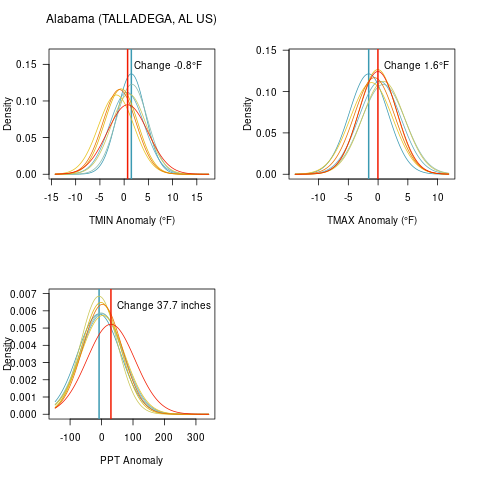
\includegraphics[width=1.00\textwidth]{/home/CAMPUS/mwl04747/github/Climate_Change_Narratives/Social_Media/png/Alabama-USC00018024-GSOM-normalPDF.png}
\caption{The changing in monthly temperature data, assuming a normal probability distribution.}
\label{fig:GSOM-normalPDF}
\end{figure}

\subsection{Using library densEstBayes}

Now, I used a screen split to look at the distribution of the temperate anomolies. First, we look at a simple histogram of the entire dataset. 

\begin{knitrout}
\definecolor{shadecolor}{rgb}{0.969, 0.969, 0.969}\color{fgcolor}\begin{kframe}
\begin{alltt}
\hlkwd{par}\hlstd{(}\hlkwc{mfrow}\hlstd{=}\hlkwd{c}\hlstd{(}\hlnum{1}\hlstd{,}\hlnum{1}\hlstd{))}
\hlkwd{hist}\hlstd{(GSOM2}\hlopt{$}\hlstd{TMIN.anom,} \hlkwc{col} \hlstd{=} \hlstr{"gold"}\hlstd{,}
     \hlkwc{main} \hlstd{=} \hlstr{""}\hlstd{,} \hlkwc{probability} \hlstd{=} \hlnum{TRUE}\hlstd{,}
     \hlkwc{xlab} \hlstd{=} \hlstr{"Minimum Temperature Anomaly (°F)"}\hlstd{)}
\end{alltt}
\end{kframe}
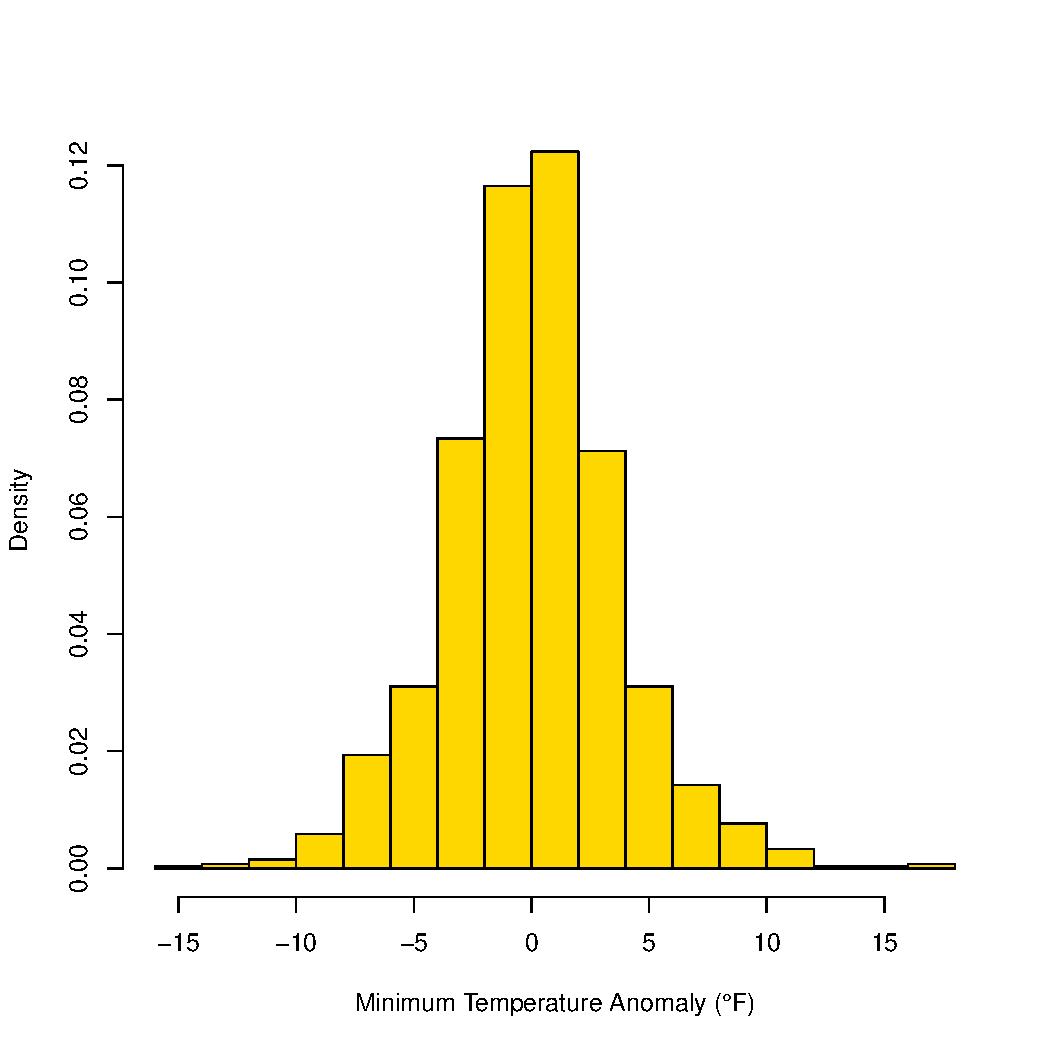
\includegraphics[width=\maxwidth]{figure/unnamed-chunk-20-1} 
\end{knitrout}

The data center around zero, as expected, but are these normally distributed? 

For TMAX there is a 0.031 probability that the distribution is the same as the normal distribution. For TMIN there is a 0 probability that the distribution is the same as the normal distribution. For PPT is a 0 probability that the distribution is the same as the normal distribution.

\begin{knitrout}
\definecolor{shadecolor}{rgb}{0.969, 0.969, 0.969}\color{fgcolor}\begin{kframe}
\begin{alltt}
\hlkwa{if}\hlstd{(}\hlkwd{shapiro.test}\hlstd{(GSOM2}\hlopt{$}\hlstd{TMAX.anom)}\hlopt{$}\hlstd{p.value}\hlopt{<}\hlnum{.05} \hlopt{|}
   \hlkwd{shapiro.test}\hlstd{(GSOM2}\hlopt{$}\hlstd{TMIN.anom)}\hlopt{$}\hlstd{p.value}\hlopt{<}\hlnum{.05} \hlopt{|}
   \hlkwd{shapiro.test}\hlstd{(GSOM2}\hlopt{$}\hlstd{PPT.anom)}\hlopt{$}\hlstd{p.value}\hlopt{<}\hlnum{.05}\hlstd{) text}\hlkwb{=}\hlstr{"to avoid "} \hlkwa{else} \hlstd{text}\hlkwb{=}\hlstr{"to use"}
\end{alltt}
\end{kframe}
\end{knitrout}

These values suggest that there is good reason to avoid  the normal probability distribution. 

Next we use a function to estimate the probability distribution using a markof chain the creates an estimated probability distribution. This doesn't always work when the distribution is not even and their only 10 years of data per slot. I suspect, I should make this by every 20 years. Plus that will go way faster and I think the data visualization will be more robust. 

\begin{knitrout}
\definecolor{shadecolor}{rgb}{0.969, 0.969, 0.969}\color{fgcolor}\begin{kframe}
\begin{alltt}
\hlkwd{setwd}\hlstd{(}\hlstr{"/home/CAMPUS/mwl04747/github/Climate_Change_Narratives/Social_Media"}\hlstd{)}

\hlkwa{if}\hlstd{(}\hlopt{!}\hlkwd{file.exists}\hlstd{(}\hlkwd{paste0}\hlstd{(}\hlstr{"png//"}\hlstd{, fips}\hlopt{$}\hlstd{State,} \hlstr{"-"}\hlstd{, stid,} \hlstr{"-GSOM-estDensity.png"}\hlstd{)))\{}
   \hlkwd{print}\hlstd{(}\hlstr{"Creating estimated density distribution"}\hlstd{)}

\hlkwd{png}\hlstd{(}\hlkwd{paste0}\hlstd{(}\hlstr{"png//"}\hlstd{, fips}\hlopt{$}\hlstd{State,} \hlstr{"-"}\hlstd{, stid,} \hlstr{"-GSOM-estDensity.png"}\hlstd{),}
    \hlkwc{width} \hlstd{=} \hlnum{480}\hlstd{,} \hlkwc{height} \hlstd{=} \hlnum{320}\hlstd{,} \hlkwc{units} \hlstd{=} \hlstr{"px"}\hlstd{,} \hlkwc{pointsize} \hlstd{=} \hlnum{12}\hlstd{,} \hlkwc{bg} \hlstd{=} \hlstr{"white"}\hlstd{)}

\hlcom{# Split Screen TMAX Legend TMIN}
\hlcom{# screen with values for left, right, bottom, and top.}
\hlkwd{split.screen}\hlstd{(}\hlkwd{rbind}\hlstd{(}\hlkwd{c}\hlstd{(}\hlnum{.01}\hlstd{,} \hlnum{0.99}\hlstd{,} \hlnum{0.86}\hlstd{,} \hlnum{0.95}\hlstd{),}
                   \hlkwd{c}\hlstd{(}\hlnum{0.01}\hlstd{,} \hlnum{0.45}\hlstd{,} \hlnum{0.01}\hlstd{,} \hlnum{0.85}\hlstd{),}
                   \hlkwd{c}\hlstd{(}\hlnum{0.45}\hlstd{,} \hlnum{0.55}\hlstd{,} \hlnum{0.01}\hlstd{,} \hlnum{0.85}\hlstd{),}
                   \hlkwd{c}\hlstd{(}\hlnum{0.55}\hlstd{,} \hlnum{0.99}\hlstd{,} \hlnum{0.01}\hlstd{,} \hlnum{0.85}\hlstd{)))}

\hlkwd{screen}\hlstd{(}\hlnum{1}\hlstd{)}
\hlkwd{par}\hlstd{(}\hlkwc{mar}\hlstd{=}\hlkwd{c}\hlstd{(}\hlnum{0}\hlstd{,}\hlnum{0}\hlstd{,}\hlnum{0}\hlstd{,}\hlnum{0}\hlstd{))}
\hlkwd{plot}\hlstd{(}\hlnum{NA}\hlstd{,} \hlkwc{xaxt}\hlstd{=}\hlstr{'n'}\hlstd{,}\hlkwc{yaxt}\hlstd{=}\hlstr{'n'}\hlstd{,}\hlkwc{bty}\hlstd{=}\hlstr{'n'}\hlstd{,}\hlkwc{ylab}\hlstd{=}\hlstr{''}\hlstd{,}\hlkwc{xlab}\hlstd{=}\hlstr{''}\hlstd{,} \hlkwc{xlim}\hlstd{=}\hlkwd{c}\hlstd{(}\hlnum{0}\hlstd{,}\hlnum{10}\hlstd{),} \hlkwc{ylim}\hlstd{=}\hlkwd{c}\hlstd{(}\hlnum{0}\hlstd{,} \hlnum{10}\hlstd{))}
\hlkwd{mtext}\hlstd{(}\hlkwd{paste0}\hlstd{(fips}\hlopt{$}\hlstd{State,} \hlstr{" ("}\hlstd{, GSOM_Longest}\hlopt{$}\hlstd{name,} \hlstr{")"}\hlstd{),} \hlkwc{side}\hlstd{=}\hlnum{3}\hlstd{,} \hlkwc{line}\hlstd{=}\hlopt{-}\hlnum{1}\hlstd{,} \hlkwc{cex}\hlstd{=}\hlnum{1.4}\hlstd{)}

\hlkwd{screen}\hlstd{(}\hlnum{2}\hlstd{)}

\hlcom{# Determine xg (range)}
\hlstd{dest} \hlkwb{<-} \hlkwd{densEstBayes}\hlstd{(GSOM2}\hlopt{$}\hlstd{TMIN.anom,} \hlkwc{method} \hlstd{=} \hlstr{"NUTS"}\hlstd{); dest}\hlopt{$}\hlstd{range.x}

\hlstd{control} \hlkwb{=} \hlkwd{densEstBayes.control}\hlstd{(}\hlkwc{range.x} \hlstd{= dest}\hlopt{$}\hlstd{range.x,}
      \hlkwc{numBins} \hlstd{=} \hlnum{401}\hlstd{,}
      \hlkwc{numBasis} \hlstd{=} \hlnum{50}\hlstd{,} \hlkwc{sigmabeta} \hlstd{=} \hlnum{1e5}\hlstd{,} \hlkwc{ssigma} \hlstd{=} \hlnum{1000}\hlstd{,}
      \hlkwc{convToler} \hlstd{=} \hlnum{1e-5}\hlstd{,} \hlkwc{maxIter} \hlstd{=} \hlnum{500}\hlstd{,} \hlkwc{nWarm} \hlstd{=} \hlkwa{NULL}\hlstd{,}
      \hlkwc{nKept} \hlstd{=} \hlkwa{NULL}\hlstd{,} \hlkwc{nThin} \hlstd{=} \hlnum{1}\hlstd{,} \hlkwc{msgCode} \hlstd{=} \hlnum{1}\hlstd{)}

\hlcom{#destSMFVB <- densEstBayes(GSOM2$TMIN.anom, method = "SMFVB", control = control)}
\hlcom{#plot(destSMFVB, plotIt=T, xlab = "TMIN", main = "", setCol=h.ramp[i])}
\hlkwd{par}\hlstd{(}\hlkwc{las}\hlstd{=}\hlnum{1}\hlstd{,} \hlkwc{mar}\hlstd{=}\hlkwd{c}\hlstd{(}\hlnum{4}\hlstd{,} \hlnum{4}\hlstd{,} \hlnum{0}\hlstd{,} \hlnum{0}\hlstd{)} \hlopt{+} \hlnum{0.1}\hlstd{)}
\hlkwa{for}\hlstd{(i} \hlkwa{in} \hlnum{1}\hlopt{:}\hlkwd{length}\hlstd{(}\hlkwd{unique}\hlstd{(GSOM2}\hlopt{$}\hlstd{Score)))\{}
   \hlcom{# i = 13}
   \hlstd{GSOM2sub} \hlkwb{=} \hlstd{GSOM2[GSOM2}\hlopt{$}\hlstd{Score}\hlopt{==}\hlkwd{sort}\hlstd{(}\hlkwd{unique}\hlstd{(GSOM2}\hlopt{$}\hlstd{Score))[i],]}
   \hlstd{dest} \hlkwb{<-} \hlkwd{densEstBayes}\hlstd{(GSOM2sub}\hlopt{$}\hlstd{TMIN.anom,} \hlkwc{method} \hlstd{=} \hlstr{"NUTS"}\hlstd{,} \hlkwc{control} \hlstd{= control)}
   \hlstd{xg} \hlkwb{=} \hlkwd{plot}\hlstd{(dest,} \hlkwc{plotIt}\hlstd{=}\hlnum{FALSE}\hlstd{)}\hlopt{$}\hlstd{xg}
   \hlstd{densEstg} \hlkwb{=} \hlkwd{plot}\hlstd{(dest,} \hlkwc{plotIt}\hlstd{=}\hlnum{FALSE}\hlstd{)}\hlopt{$}\hlstd{densEstg}

   \hlkwa{if}\hlstd{(i}\hlopt{==}\hlnum{1}\hlstd{)} \hlkwd{plot}\hlstd{(}\hlnum{0}\hlstd{,} \hlkwc{type} \hlstd{=} \hlstr{"n"}\hlstd{,} \hlkwc{bty} \hlstd{=} \hlstr{"l"}\hlstd{,}
         \hlkwc{xlim}\hlstd{=}\hlkwd{range}\hlstd{(xg),} \hlkwc{ylim}\hlstd{=}\hlkwd{c}\hlstd{(}\hlnum{0}\hlstd{,}\hlnum{0.25}\hlstd{),}
         \hlkwc{xlab} \hlstd{=} \hlstr{"TMIN anomaly (°F)"}\hlstd{,} \hlkwc{main} \hlstd{=} \hlstr{""}\hlstd{,} \hlkwc{ylab}\hlstd{=}\hlstr{"Density"}\hlstd{)}
   \hlkwd{lines}\hlstd{(xg, densEstg,} \hlkwc{col}\hlstd{=h.ramp[i])}
\hlkwd{rug}\hlstd{(}\hlkwd{jitter}\hlstd{(GSOM2sub}\hlopt{$}\hlstd{TMIN.anom,}\hlkwc{amount} \hlstd{=} \hlnum{0.2}\hlstd{),} \hlkwc{col}\hlstd{=h.ramp[i])}
\hlstd{\}}

\hlkwd{screen}\hlstd{(}\hlnum{3}\hlstd{)}
\hlkwd{par}\hlstd{(}\hlkwc{mar}\hlstd{=}\hlkwd{c}\hlstd{(}\hlnum{0}\hlstd{,}\hlnum{0}\hlstd{,}\hlnum{1}\hlstd{,}\hlnum{0}\hlstd{))}
\hlkwd{plot}\hlstd{(}\hlnum{NA}\hlstd{,}\hlkwc{xaxt}\hlstd{=}\hlstr{'n'}\hlstd{,}\hlkwc{yaxt}\hlstd{=}\hlstr{'n'}\hlstd{,}\hlkwc{bty}\hlstd{=}\hlstr{'n'}\hlstd{,}\hlkwc{ylab}\hlstd{=}\hlstr{''}\hlstd{,}\hlkwc{xlab}\hlstd{=}\hlstr{''}\hlstd{,} \hlkwc{xlim}\hlstd{=}\hlkwd{c}\hlstd{(}\hlnum{0}\hlstd{,}\hlnum{10}\hlstd{),} \hlkwc{ylim}\hlstd{=}\hlkwd{c}\hlstd{(}\hlnum{0}\hlstd{,}\hlnum{10}\hlstd{))}
\hlcom{# }
\hlkwd{legend}\hlstd{(}\hlstr{"topright"}\hlstd{,} \hlkwc{inset}\hlstd{=}\hlkwd{c}\hlstd{(}\hlnum{0}\hlstd{,}\hlnum{0}\hlstd{),} \hlkwc{bg}\hlstd{=}\hlstr{"transparent"}\hlstd{,} \hlkwc{bty}\hlstd{=}\hlstr{"n"}\hlstd{,}
       \hlkwc{legend}\hlstd{=}\hlkwd{unique}\hlstd{(GSOM2}\hlopt{$}\hlstd{Score),}
       \hlkwc{fill}\hlstd{=h.ramp,} \hlkwc{horiz}\hlstd{=}\hlnum{FALSE}\hlstd{,} \hlkwc{cex}\hlstd{=}\hlnum{0.85}\hlstd{)}

\hlkwd{screen}\hlstd{(}\hlnum{4}\hlstd{)}
\hlkwd{par}\hlstd{(}\hlkwc{las}\hlstd{=}\hlnum{1}\hlstd{,} \hlkwc{mar}\hlstd{=}\hlkwd{c}\hlstd{(}\hlnum{4}\hlstd{,} \hlnum{4}\hlstd{,} \hlnum{0}\hlstd{,} \hlnum{0}\hlstd{)} \hlopt{+}\hlnum{0.1}\hlstd{)}
\hlcom{# Determine xg (range)}
\hlstd{dest} \hlkwb{<-} \hlkwd{densEstBayes}\hlstd{(GSOM2}\hlopt{$}\hlstd{TMAX.anom,} \hlkwc{method} \hlstd{=} \hlstr{"NUTS"}\hlstd{); dest}\hlopt{$}\hlstd{range.x}

\hlstd{control} \hlkwb{=} \hlkwd{densEstBayes.control}\hlstd{(}\hlkwc{range.x} \hlstd{= dest}\hlopt{$}\hlstd{range.x,}
      \hlkwc{numBins} \hlstd{=} \hlnum{401}\hlstd{,}
      \hlkwc{numBasis} \hlstd{=} \hlnum{50}\hlstd{,} \hlkwc{sigmabeta} \hlstd{=} \hlnum{1e5}\hlstd{,} \hlkwc{ssigma} \hlstd{=} \hlnum{1000}\hlstd{,}
      \hlkwc{convToler} \hlstd{=} \hlnum{1e-5}\hlstd{,} \hlkwc{maxIter} \hlstd{=} \hlnum{500}\hlstd{,} \hlkwc{nWarm} \hlstd{=} \hlkwa{NULL}\hlstd{,}
      \hlkwc{nKept} \hlstd{=} \hlkwa{NULL}\hlstd{,} \hlkwc{nThin} \hlstd{=} \hlnum{1}\hlstd{,} \hlkwc{msgCode} \hlstd{=} \hlnum{1}\hlstd{)}

\hlkwa{for}\hlstd{(i} \hlkwa{in} \hlnum{1}\hlopt{:}\hlkwd{length}\hlstd{(}\hlkwd{unique}\hlstd{(GSOM2}\hlopt{$}\hlstd{Score)))\{}
   \hlcom{# i = 13}
   \hlstd{GSOM2sub} \hlkwb{=} \hlstd{GSOM2[GSOM2}\hlopt{$}\hlstd{Score}\hlopt{==}\hlkwd{sort}\hlstd{(}\hlkwd{unique}\hlstd{(GSOM2}\hlopt{$}\hlstd{Score))[i],]}
   \hlstd{dest} \hlkwb{<-} \hlkwd{densEstBayes}\hlstd{(GSOM2sub}\hlopt{$}\hlstd{TMAX.anom,} \hlkwc{method} \hlstd{=} \hlstr{"NUTS"}\hlstd{,} \hlkwc{control} \hlstd{= control)}
   \hlstd{xg} \hlkwb{=} \hlkwd{plot}\hlstd{(dest,} \hlkwc{plotIt}\hlstd{=}\hlnum{FALSE}\hlstd{)}\hlopt{$}\hlstd{xg}
   \hlstd{densEstg} \hlkwb{=} \hlkwd{plot}\hlstd{(dest,} \hlkwc{plotIt}\hlstd{=}\hlnum{FALSE}\hlstd{)}\hlopt{$}\hlstd{densEstg}

   \hlkwa{if}\hlstd{(i}\hlopt{==}\hlnum{1}\hlstd{)} \hlkwd{plot}\hlstd{(}\hlnum{0}\hlstd{,} \hlkwc{type} \hlstd{=} \hlstr{"n"}\hlstd{,} \hlkwc{bty} \hlstd{=} \hlstr{"l"}\hlstd{,}
         \hlkwc{xlim}\hlstd{=}\hlkwd{range}\hlstd{(xg),} \hlkwc{ylim}\hlstd{=}\hlkwd{c}\hlstd{(}\hlnum{0}\hlstd{,}\hlnum{.25}\hlstd{),}
         \hlkwc{xlab} \hlstd{=} \hlstr{"TMAX anomaly (°F)"}\hlstd{,} \hlkwc{main} \hlstd{=} \hlstr{""}\hlstd{,} \hlkwc{ylab}\hlstd{=}\hlstr{"Density"}\hlstd{)}
   \hlkwd{lines}\hlstd{(xg, densEstg,} \hlkwc{col}\hlstd{=h.ramp[i])}
\hlkwd{rug}\hlstd{(}\hlkwd{jitter}\hlstd{(GSOM2sub}\hlopt{$}\hlstd{TMIN.anom,}\hlkwc{amount} \hlstd{=} \hlnum{0.2}\hlstd{),} \hlkwc{col}\hlstd{=h.ramp[i])}
\hlstd{\}}
\hlcom{#rug(jitter(GSOM2sub$TMIN.anom,amount = 0.2), col=h.ramp[i])}

\hlkwd{close.screen}\hlstd{(}\hlkwc{all.screens} \hlstd{=} \hlnum{TRUE}\hlstd{)}
\hlkwd{dev.off}\hlstd{()}
\hlstd{\}} \hlkwa{else} \hlstd{\{}
   \hlkwd{print}\hlstd{(}\hlstr{"Skipping estimated density distribution chunk"}\hlstd{)\}}
\end{alltt}
\end{kframe}
\end{knitrout}

The process to create these figures is very time consuming, so in general, I need to come up with an if then statement to avoid creating these everytime!

\begin{figure}
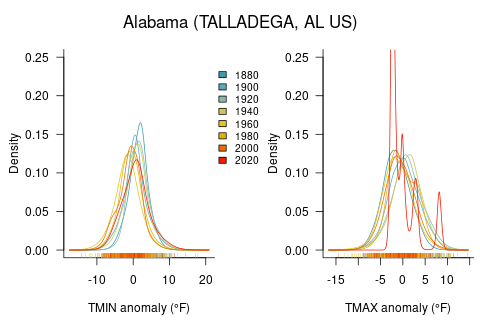
\includegraphics[width=1.00\textwidth]{/home/CAMPUS/mwl04747/github/Climate_Change_Narratives/Social_Media/png/Alabama-USC00018024-GSOM-estDensity.png}
\caption{The changing in monthly temperature data.}
\label{fig:GSOM-estDensity}
\end{figure}

\section{Animated GIFs}

So far, this creates a gif file, but I haven't been able get the gif in the pdf directly yet. I will need an additional package or create separate png that are combined. For now, we'll create a gif file to be used in separate documents.

\subsection{Probability Distributions}

\begin{knitrout}
\definecolor{shadecolor}{rgb}{0.969, 0.969, 0.969}\color{fgcolor}\begin{kframe}
\begin{alltt}
\hlkwd{setwd}\hlstd{(}\hlstr{"/home/CAMPUS/mwl04747/github/Climate_Change_Narratives/docs/"}\hlstd{)}
\hlkwa{if}\hlstd{(}\hlopt{!}\hlkwd{file.exists}\hlstd{(}\hlkwd{paste0}\hlstd{(}\hlstr{"Climate_gifs/"}\hlstd{,}
   \hlstd{fips}\hlopt{$}\hlstd{State,} \hlstr{"-"}\hlstd{, stid,} \hlstr{"_GSOM-normalPDF.gif"}\hlstd{)))\{}
   \hlkwd{print}\hlstd{(}\hlstr{"Creating animated normal probability "}\hlstd{)}

\hlcom{# Define an image_graph size}
\hlstd{img} \hlkwb{<-} \hlkwd{image_graph}\hlstd{(}\hlnum{600}\hlstd{,} \hlnum{480}\hlstd{,} \hlkwc{res} \hlstd{=} \hlnum{96}\hlstd{)}

\hlcom{# START ------------------------------------------}

\hlstd{ylim_new}\hlkwb{=}\hlnum{NA}
\hlkwa{for}\hlstd{(i} \hlkwa{in} \hlnum{1}\hlopt{:}\hlkwd{length}\hlstd{(}\hlkwd{unique}\hlstd{(GSOM2}\hlopt{$}\hlstd{Decade)))}
   \hlstd{\{}
\hlcom{# i = 9}
\hlstd{decade}\hlkwb{=}\hlstd{(}\hlkwd{unique}\hlstd{(GSOM2}\hlopt{$}\hlstd{Decade))[}\hlkwd{order}\hlstd{(}\hlkwd{unique}\hlstd{(GSOM2}\hlopt{$}\hlstd{Decade))}\hlopt{==}\hlstd{i]}

\hlstd{GSOM2sub} \hlkwb{<-} \hlstd{GSOM2[GSOM2}\hlopt{$}\hlstd{Decade}\hlopt{==}\hlstd{decade,]}
\hlstd{h.ramp} \hlkwb{<-} \hlkwd{rev}\hlstd{(}\hlkwd{heat.colors}\hlstd{(}\hlkwd{length}\hlstd{(}\hlkwd{unique}\hlstd{(GSOM2}\hlopt{$}\hlstd{Decade))}\hlopt{+}\hlnum{1}\hlstd{))[}\hlopt{-}\hlnum{1}\hlstd{]}

\hlcom{# Determine Stats for PDFs}
\hlstd{TMAX.mean.anomaly.decade} \hlkwb{=} \hlkwd{aggregate}\hlstd{(TMAX.anom} \hlopt{~} \hlstd{Decade, GSOM2sub, mean)}
\hlstd{TMAX.sd.anomaly.decade} \hlkwb{=} \hlkwd{aggregate}\hlstd{(TMAX.anom} \hlopt{~} \hlstd{Decade, GSOM2sub, sd)}
\hlkwd{names}\hlstd{(TMAX.sd.anomaly.decade)}\hlkwb{=}\hlkwd{c}\hlstd{(}\hlstr{"Decade"}\hlstd{,} \hlstr{"TMAX.sd.anom"}\hlstd{)}
\hlstd{TMIN.mean.anomaly.decade} \hlkwb{=} \hlkwd{aggregate}\hlstd{(TMIN.anom} \hlopt{~} \hlstd{Decade, GSOM2sub, mean)}
\hlstd{TMIN.sd.anomaly.decade} \hlkwb{=} \hlkwd{aggregate}\hlstd{(TMIN.anom} \hlopt{~} \hlstd{Decade, GSOM2sub, sd)}
\hlkwd{names}\hlstd{(TMIN.sd.anomaly.decade)}\hlkwb{=}\hlkwd{c}\hlstd{(}\hlstr{"Decade"}\hlstd{,} \hlstr{"TMIN.sd.anom"}\hlstd{)}

\hlstd{TMAX.temp} \hlkwb{=} \hlkwd{merge}\hlstd{(TMAX.mean.anomaly.decade, TMAX.sd.anomaly.decade,} \hlkwc{by}\hlstd{=}\hlstr{"Decade"}\hlstd{)}

\hlstd{TMIN.temp} \hlkwb{=} \hlkwd{merge}\hlstd{(TMIN.mean.anomaly.decade, TMIN.sd.anomaly.decade,} \hlkwc{by}\hlstd{=}\hlstr{"Decade"}\hlstd{)}

\hlstd{GSOM.Monthly.Anom.mean.sd} \hlkwb{=} \hlkwd{merge}\hlstd{(TMAX.temp, TMIN.temp,} \hlkwc{by}\hlstd{=}\hlstr{"Decade"}\hlstd{)}

\hlkwd{par}\hlstd{(}\hlkwc{las}\hlstd{=}\hlnum{1}\hlstd{,} \hlkwc{mfrow}\hlstd{=}\hlkwd{c}\hlstd{(}\hlnum{1}\hlstd{,}\hlnum{2}\hlstd{),} \hlkwc{mar}\hlstd{=} \hlkwd{c}\hlstd{(}\hlnum{4}\hlstd{,} \hlnum{4}\hlstd{,} \hlnum{2}\hlstd{,} \hlnum{1}\hlstd{)} \hlopt{+} \hlnum{0.1}\hlstd{)}

\hlstd{Anom.x} \hlkwb{=} \hlkwd{seq}\hlstd{(}\hlkwd{min}\hlstd{(GSOM2}\hlopt{$}\hlstd{TMAX.anom),} \hlkwd{max}\hlstd{(GSOM2}\hlopt{$}\hlstd{TMAX.anom),} \hlkwc{by}\hlstd{=}\hlnum{.1}\hlstd{)}
\hlkwd{plot}\hlstd{(Anom.x,} \hlkwd{dnorm}\hlstd{(Anom.x,} \hlkwc{mean}\hlstd{=GSOM.Monthly.Anom.mean.sd}\hlopt{$}\hlstd{TMAX.anom[}\hlnum{1}\hlstd{],}
   \hlkwc{sd}\hlstd{=GSOM.Monthly.Anom.mean.sd}\hlopt{$}\hlstd{TMAX.sd.anom[}\hlnum{1}\hlstd{]),} \hlkwc{ty}\hlstd{=}\hlstr{"l"}\hlstd{,} \hlkwc{col}\hlstd{=h.ramp[i],} \hlkwc{ylab}\hlstd{=}\hlstr{"Density"}\hlstd{,} \hlkwc{xlab}\hlstd{=}\hlstr{"TMAX Anomaly"}\hlstd{)}
\hlkwd{abline}\hlstd{(}\hlkwc{v}\hlstd{=}\hlkwd{mean}\hlstd{(GSOM2}\hlopt{$}\hlstd{TMAX.anom[GSOM2}\hlopt{$}\hlstd{Decade}\hlopt{==}\hlkwd{min}\hlstd{(GSOM}\hlopt{$}\hlstd{Decade)]))}
\hlkwd{mtext}\hlstd{(}\hlkwd{paste0}\hlstd{(fips}\hlopt{$}\hlstd{State,} \hlstr{" "}\hlstd{, decade),} \hlkwc{side}\hlstd{=}\hlnum{3}\hlstd{)}

\hlstd{Anom.x} \hlkwb{=} \hlkwd{seq}\hlstd{(}\hlkwd{min}\hlstd{(GSOM2}\hlopt{$}\hlstd{TMIN.anom),} \hlkwd{max}\hlstd{(GSOM2}\hlopt{$}\hlstd{TMIN.anom),} \hlkwc{by}\hlstd{=}\hlnum{.1}\hlstd{)}
\hlkwd{plot}\hlstd{(Anom.x,} \hlkwd{dnorm}\hlstd{(Anom.x,} \hlkwc{mean}\hlstd{=GSOM.Monthly.Anom.mean.sd}\hlopt{$}\hlstd{TMIN.anom[}\hlnum{1}\hlstd{],}
   \hlkwc{sd}\hlstd{=GSOM.Monthly.Anom.mean.sd}\hlopt{$}\hlstd{TMIN.sd.anom[}\hlnum{1}\hlstd{]),} \hlkwc{ty}\hlstd{=}\hlstr{"l"}\hlstd{,} \hlkwc{col}\hlstd{=h.ramp[i],} \hlkwc{ylab}\hlstd{=}\hlstr{"Density"}\hlstd{,} \hlkwc{xlab}\hlstd{=}\hlstr{"TMIN Anomaly"}\hlstd{)}
\hlkwd{abline}\hlstd{(}\hlkwc{v}\hlstd{=}\hlkwd{mean}\hlstd{(GSOM2}\hlopt{$}\hlstd{TMIN.anom[GSOM2}\hlopt{$}\hlstd{Decade}\hlopt{==}\hlkwd{min}\hlstd{(GSOM}\hlopt{$}\hlstd{Decade)]))}
\hlkwd{mtext}\hlstd{(}\hlkwd{paste0}\hlstd{(fips}\hlopt{$}\hlstd{State,} \hlstr{" "}\hlstd{, decade),} \hlkwc{side}\hlstd{=}\hlnum{3}\hlstd{)}
\hlstd{\}}

\hlkwd{par}\hlstd{(}\hlkwc{las}\hlstd{=}\hlnum{1}\hlstd{,} \hlkwc{mfrow}\hlstd{=}\hlkwd{c}\hlstd{(}\hlnum{1}\hlstd{,}\hlnum{2}\hlstd{),} \hlkwc{mar}\hlstd{=} \hlkwd{c}\hlstd{(}\hlnum{4}\hlstd{,} \hlnum{4}\hlstd{,} \hlnum{2}\hlstd{,} \hlnum{1}\hlstd{)} \hlopt{+} \hlnum{0.1}\hlstd{)}

\hlstd{TMAX.anomaly.decade} \hlkwb{=} \hlkwd{aggregate}\hlstd{(TMAX.anom} \hlopt{~} \hlstd{Decade, GSOM2,}
   \hlkwc{FUN} \hlstd{=} \hlkwa{function}\hlstd{(}\hlkwc{x}\hlstd{)} \hlkwd{c}\hlstd{(}\hlkwc{mean} \hlstd{=} \hlkwd{mean}\hlstd{(x),} \hlkwc{sd} \hlstd{=} \hlkwd{sd}\hlstd{(x)))}
\hlstd{TMIN.anomaly.decade} \hlkwb{=} \hlkwd{aggregate}\hlstd{(TMIN.anom} \hlopt{~} \hlstd{Decade, GSOM2,}
   \hlkwc{FUN} \hlstd{=} \hlkwa{function}\hlstd{(}\hlkwc{x}\hlstd{)} \hlkwd{c}\hlstd{(}\hlkwc{mean} \hlstd{=} \hlkwd{mean}\hlstd{(x),} \hlkwc{sd} \hlstd{=} \hlkwd{sd}\hlstd{(x)))}


\hlstd{Anom.x} \hlkwb{=} \hlkwd{seq}\hlstd{(}\hlkwd{min}\hlstd{(GSOM2}\hlopt{$}\hlstd{TMIN.anom),} \hlkwd{max}\hlstd{(GSOM2}\hlopt{$}\hlstd{TMIN.anom),} \hlkwc{by}\hlstd{=}\hlnum{.1}\hlstd{)}
\hlkwd{plot}\hlstd{(Anom.x,} \hlkwd{dnorm}\hlstd{(Anom.x,} \hlkwc{mean}\hlstd{=TMIN.anomaly.decade}\hlopt{$}\hlstd{TMIN.anom[[}\hlnum{1}\hlstd{,}\hlnum{1}\hlstd{]],}
   \hlkwc{sd}\hlstd{=TMIN.anomaly.decade}\hlopt{$}\hlstd{TMIN.anom[[}\hlnum{1}\hlstd{,}\hlnum{2}\hlstd{]]),} \hlkwc{ty}\hlstd{=}\hlstr{"l"}\hlstd{,} \hlkwc{col}\hlstd{=h.ramp[}\hlnum{1}\hlstd{],} \hlkwc{ylab}\hlstd{=}\hlstr{"Density"}\hlstd{,} \hlkwc{xlab}\hlstd{=}\hlstr{"TMIN Anomaly"}\hlstd{)}
\hlkwd{mtext}\hlstd{(}\hlkwd{paste0}\hlstd{(fips}\hlopt{$}\hlstd{State,} \hlstr{" "}\hlstd{, decade),} \hlkwc{side}\hlstd{=}\hlnum{3}\hlstd{)}
\hlkwa{for}\hlstd{(i} \hlkwa{in} \hlnum{2}\hlopt{:}\hlkwd{nrow}\hlstd{(TMIN.anomaly.decade))\{}
\hlkwd{lines}\hlstd{(Anom.x,} \hlkwd{dnorm}\hlstd{(Anom.x,} \hlkwc{mean}\hlstd{=TMIN.anomaly.decade}\hlopt{$}\hlstd{TMIN.anom[[i,}\hlnum{1}\hlstd{]],} \hlkwc{sd}\hlstd{=TMIN.anomaly.decade}\hlopt{$}\hlstd{TMIN.anom[[i,}\hlnum{2}\hlstd{]]),} \hlkwc{col}\hlstd{=h.ramp[i])}
\hlstd{\}}
\hlkwd{abline}\hlstd{(}\hlkwc{v}\hlstd{=}\hlkwd{mean}\hlstd{(GSOM2}\hlopt{$}\hlstd{TMIN.anom[GSOM2}\hlopt{$}\hlstd{Decade}\hlopt{==}\hlkwd{min}\hlstd{(GSOM}\hlopt{$}\hlstd{Decade)]),} \hlkwc{col}\hlstd{=}\hlstr{"blue"}\hlstd{)}
\hlkwd{abline}\hlstd{(}\hlkwc{v}\hlstd{=}\hlkwd{mean}\hlstd{(GSOM2}\hlopt{$}\hlstd{TMIN.anom[GSOM2}\hlopt{$}\hlstd{Decade}\hlopt{==}\hlkwd{max}\hlstd{(GSOM}\hlopt{$}\hlstd{Decade)]),} \hlkwc{col}\hlstd{=}\hlstr{"red"}\hlstd{)}

\hlstd{Anom.x} \hlkwb{=} \hlkwd{seq}\hlstd{(}\hlkwd{min}\hlstd{(GSOM2}\hlopt{$}\hlstd{TMAX.anom),} \hlkwd{max}\hlstd{(GSOM2}\hlopt{$}\hlstd{TMAX.anom),} \hlkwc{by}\hlstd{=}\hlnum{.1}\hlstd{)}
\hlkwd{plot}\hlstd{(Anom.x,} \hlkwd{dnorm}\hlstd{(Anom.x,} \hlkwc{mean}\hlstd{=TMAX.anomaly.decade}\hlopt{$}\hlstd{TMAX.anom[[}\hlnum{1}\hlstd{,}\hlnum{1}\hlstd{]],}
   \hlkwc{sd}\hlstd{=TMAX.anomaly.decade}\hlopt{$}\hlstd{TMAX.anom[[}\hlnum{1}\hlstd{,}\hlnum{2}\hlstd{]]),} \hlkwc{ty}\hlstd{=}\hlstr{"l"}\hlstd{,} \hlkwc{col}\hlstd{=h.ramp[}\hlnum{1}\hlstd{],} \hlkwc{ylab}\hlstd{=}\hlstr{"Density"}\hlstd{,} \hlkwc{xlab}\hlstd{=}\hlstr{"TMAX Anomaly"}\hlstd{)}
\hlkwd{mtext}\hlstd{(}\hlkwd{paste0}\hlstd{(fips}\hlopt{$}\hlstd{State,} \hlstr{" "}\hlstd{, decade),} \hlkwc{side}\hlstd{=}\hlnum{3}\hlstd{)}
\hlkwa{for}\hlstd{(i} \hlkwa{in} \hlnum{2}\hlopt{:}\hlkwd{nrow}\hlstd{(TMAX.anomaly.decade))\{}
\hlkwd{lines}\hlstd{(Anom.x,} \hlkwd{dnorm}\hlstd{(Anom.x,} \hlkwc{mean}\hlstd{=TMAX.anomaly.decade}\hlopt{$}\hlstd{TMAX.anom[[i,}\hlnum{1}\hlstd{]],} \hlkwc{sd}\hlstd{=TMAX.anomaly.decade}\hlopt{$}\hlstd{TMAX.anom[[i,}\hlnum{2}\hlstd{]]),} \hlkwc{col}\hlstd{=h.ramp[i])}
\hlstd{\}}
\hlkwd{abline}\hlstd{(}\hlkwc{v}\hlstd{=}\hlkwd{mean}\hlstd{(GSOM2}\hlopt{$}\hlstd{TMAX.anom[GSOM2}\hlopt{$}\hlstd{Decade}\hlopt{==}\hlkwd{min}\hlstd{(GSOM}\hlopt{$}\hlstd{Decade)]),} \hlkwc{col}\hlstd{=}\hlstr{"blue"}\hlstd{)}
\hlkwd{abline}\hlstd{(}\hlkwc{v}\hlstd{=}\hlkwd{mean}\hlstd{(GSOM2}\hlopt{$}\hlstd{TMAX.anom[GSOM2}\hlopt{$}\hlstd{Decade}\hlopt{==}\hlkwd{max}\hlstd{(GSOM}\hlopt{$}\hlstd{Decade)]),} \hlkwc{col}\hlstd{=}\hlstr{"red"}\hlstd{)}


\hlcom{# END -----------------------------------------------------}
\hlkwd{dev.off}\hlstd{()}

\hlstd{GSOM_animation} \hlkwb{<-} \hlkwd{image_animate}\hlstd{(img,} \hlkwc{fps} \hlstd{=} \hlnum{1}\hlstd{,} \hlkwc{loop}\hlstd{=}\hlnum{2}\hlstd{,} \hlkwc{optimize} \hlstd{=} \hlnum{TRUE}\hlstd{)}
\hlcom{#print(GSOM_animation)}
\hlkwd{setwd}\hlstd{(}\hlstr{"/home/CAMPUS/mwl04747/github/Climate_Change_Narratives/docs/"}\hlstd{)}
\hlkwd{image_write}\hlstd{(GSOM_animation,} \hlkwd{paste}\hlstd{(}\hlstr{"Climate_gifs/"}\hlstd{,}
   \hlstd{fips}\hlopt{$}\hlstd{State,} \hlstr{"-"}\hlstd{, stid,} \hlstr{"_GSOM-normalPDF.gif"}\hlstd{,} \hlkwc{sep}\hlstd{=}\hlstr{""}\hlstd{))}

\hlstd{\}} \hlkwa{else} \hlstd{\{}
   \hlkwd{print}\hlstd{(}\hlstr{"Skipping animated normal distribution chunk"}\hlstd{)\}}
\end{alltt}
\end{kframe}
\end{knitrout}


The file is saved in the main directory. 


\subsection{4 Weather Trend Plots}

\begin{knitrout}
\definecolor{shadecolor}{rgb}{0.969, 0.969, 0.969}\color{fgcolor}\begin{kframe}
\begin{alltt}
\hlkwd{setwd}\hlstd{(}\hlstr{"/home/CAMPUS/mwl04747/github/Climate_Change_Narratives/docs/"}\hlstd{)}

\hlkwa{if}\hlstd{(}\hlopt{!}\hlkwd{file.exists}\hlstd{(}\hlkwd{paste0}\hlstd{(}\hlstr{"Climate_gifs/"}\hlstd{, fips}\hlopt{$}\hlstd{State,} \hlstr{"-"}\hlstd{, stid,} \hlstr{"_GSOM-4plots.gif"}\hlstd{)))\{}
   \hlkwd{print}\hlstd{(}\hlstr{"Creating animated GSOM-4plots.gif"}\hlstd{)}

\hlstd{img} \hlkwb{<-} \hlkwd{image_graph}\hlstd{(}\hlnum{600}\hlstd{,} \hlnum{480}\hlstd{,} \hlkwc{res} \hlstd{=} \hlnum{96}\hlstd{)}
\hlcom{# START ----}
\hlstd{ylim_new}\hlkwb{=}\hlnum{NA}
\hlkwa{for}\hlstd{(i} \hlkwa{in} \hlkwd{seq}\hlstd{(}\hlkwd{min}\hlstd{(GSOM}\hlopt{$}\hlstd{Year),} \hlkwd{max}\hlstd{(GSOM}\hlopt{$}\hlstd{Year),} \hlkwc{by}\hlstd{=}\hlnum{2}\hlstd{))}
   \hlstd{\{}
\hlkwd{par}\hlstd{(}\hlkwc{las}\hlstd{=}\hlnum{1}\hlstd{,} \hlkwc{mfrow}\hlstd{=}\hlkwd{c}\hlstd{(}\hlnum{4}\hlstd{,}\hlnum{1}\hlstd{),} \hlkwc{mar}\hlstd{=} \hlkwd{c}\hlstd{(}\hlnum{4}\hlstd{,} \hlnum{4}\hlstd{,} \hlnum{2}\hlstd{,} \hlnum{1}\hlstd{)} \hlopt{+} \hlnum{0.1}\hlstd{)}
\hlcom{# TMINmonthMax}
   \hlstd{GSOMsub} \hlkwb{<-} \hlstd{GSOM[GSOM}\hlopt{$}\hlstd{Month}\hlopt{==}\hlstd{TMINmonthMax} \hlopt{&} \hlstd{GSOM}\hlopt{$}\hlstd{Year}\hlopt{<=}\hlstd{i,]}
   \hlkwa{if}\hlstd{(}\hlkwd{nrow}\hlstd{(GSOMsub)}\hlopt{<}\hlnum{10}\hlstd{)} \hlkwa{next}
\hlkwd{plot}\hlstd{(TMIN}\hlopt{~}\hlstd{Date, GSOMsub[GSOMsub}\hlopt{$}\hlstd{Month}\hlopt{==}\hlstd{TMINmonthMax,],}
   \hlkwc{col}\hlstd{=}\hlstr{'gray70'}\hlstd{,} \hlkwc{pch}\hlstd{=}\hlnum{20}\hlstd{,} \hlkwc{xlab}\hlstd{=}\hlstr{""}\hlstd{,}
   \hlkwc{main}\hlstd{=}\hlkwd{paste}\hlstd{(}\hlstr{"Mean"}\hlstd{,} \hlkwd{format}\hlstd{(GSOMsub}\hlopt{$}\hlstd{Date,}\hlstr{"%B"}\hlstd{)[}\hlnum{1}\hlstd{],}
              \hlstr{"Min. Temp"}\hlstd{, GSOM_Longest}\hlopt{$}\hlstd{name))}
\hlstd{GSOM.lm} \hlkwb{=} \hlkwd{lm}\hlstd{(TMIN}\hlopt{~}\hlstd{Date, GSOMsub)}
\hlstd{pred_dates} \hlkwb{<-}\hlkwd{data.frame}\hlstd{(}\hlkwc{Date} \hlstd{= GSOMsub}\hlopt{$}\hlstd{Date);}
\hlkwd{nrow}\hlstd{(pred_dates); pred_dates}
\hlcom{#Predits the values with confidence interval }
\hlstd{ci} \hlkwb{<-} \hlkwd{predict}\hlstd{(GSOM.lm,} \hlkwc{newdata} \hlstd{= pred_dates,}
              \hlkwc{interval} \hlstd{=} \hlstr{'confidence'}\hlstd{)}
\hlkwd{lines}\hlstd{(pred_dates}\hlopt{$}\hlstd{Date,} \hlkwd{as.numeric}\hlstd{(ci[,}\hlnum{1}\hlstd{]),} \hlkwc{col}\hlstd{=}\hlstr{"darkred"}\hlstd{)}
\hlkwd{lines}\hlstd{(pred_dates}\hlopt{$}\hlstd{Date,} \hlkwd{as.numeric}\hlstd{(ci[,}\hlnum{2}\hlstd{]),} \hlkwc{col}\hlstd{=}\hlstr{"darkorange"}\hlstd{)}
\hlkwd{lines}\hlstd{(pred_dates}\hlopt{$}\hlstd{Date, ci[,}\hlnum{3}\hlstd{],} \hlkwc{col}\hlstd{=}\hlstr{"darkorange"}\hlstd{)}
\hlstd{location_index} \hlkwb{=} \hlkwd{round}\hlstd{(}\hlkwd{length}\hlstd{(GSOMsub}\hlopt{$}\hlstd{Date)} \hlopt{*} \hlnum{0.99}\hlstd{,}\hlnum{0}\hlstd{)}
\hlkwd{text}\hlstd{(pred_dates}\hlopt{$}\hlstd{Date[location_index], ci[location_index,}\hlnum{3}\hlstd{],}
     \hlkwd{paste}\hlstd{(}\hlkwd{report_prob2}\hlstd{(GSOM.lm)),} \hlkwc{pos}\hlstd{=}\hlnum{2}\hlstd{,} \hlkwc{cex}\hlstd{=}\hlnum{1.5}\hlstd{)}

\hlcom{# Box Plot of TMAX by Month}
\hlstd{CHCNDsub} \hlkwb{=} \hlkwd{subset}\hlstd{(CHCND, CHCND}\hlopt{$}\hlstd{Year}\hlopt{<=}\hlstd{i,}
      \hlkwc{select}\hlstd{=}\hlkwd{c}\hlstd{(Month, Month.name, TMAX, TMIN))}
\hlkwd{boxplot}\hlstd{(TMAX} \hlopt{~} \hlstd{Month.name,} \hlkwc{data}\hlstd{=CHCNDsub,} \hlkwc{main}\hlstd{=}\hlstr{""}\hlstd{)}
\hlstd{symbol.y} \hlkwb{=} \hlstd{(}\hlkwd{par}\hlstd{()}\hlopt{$}\hlstd{yaxp[}\hlnum{2}\hlstd{])}\hlopt{-}\hlkwd{diff}\hlstd{(}\hlkwd{par}\hlstd{()}\hlopt{$}\hlstd{yaxp[}\hlnum{1}\hlopt{:}\hlnum{2}\hlstd{])}\hlopt{*}\hlnum{.99}
\hlcom{#symbol.y = (par()$yaxp[2])}
\hlkwd{text}\hlstd{(sumstats}\hlopt{$}\hlstd{Month, symbol.y, sumstats}\hlopt{$}\hlstd{TMAX_Symbol,}
     \hlkwc{col}\hlstd{=}\hlstr{"red"}\hlstd{,} \hlkwc{cex}\hlstd{=}\hlnum{2}\hlstd{)}
\hlkwd{mtext}\hlstd{(}\hlkwd{paste}\hlstd{(}\hlstr{"Maximum Daily Temperatures"}\hlstd{,} \hlkwd{min}\hlstd{(CHCND}\hlopt{$}\hlstd{Year),}
      \hlstr{"-"}\hlstd{, i, GSOM_Longest}\hlopt{$}\hlstd{name),} \hlkwc{line}\hlstd{=}\hlnum{1}\hlstd{)}
\hlkwd{mtext}\hlstd{(}\hlstr{"(NOTE: Red astrisks correspond to signficant changes)"}\hlstd{,}
      \hlkwc{line}\hlstd{=}\hlnum{0}\hlstd{,} \hlkwc{cex}\hlstd{=}\hlnum{.7}\hlstd{)}

\hlcom{# TMAXmonthMax }
\hlstd{GSOMsub} \hlkwb{<-} \hlstd{GSOM[GSOM}\hlopt{$}\hlstd{Month}\hlopt{==}\hlstd{TMAXmonthMax} \hlopt{&} \hlstd{GSOM}\hlopt{$}\hlstd{Year}\hlopt{<=}\hlstd{i,]}
\hlstd{ylim} \hlkwb{=} \hlkwd{range}\hlstd{(GSOMsub}\hlopt{$}\hlstd{TMAX)}
\hlcom{#if(!is.na(ylim_new)) ylim[2]=ylim_new}
\hlkwd{plot}\hlstd{(TMAX}\hlopt{~}\hlstd{Date, GSOMsub,} \hlkwc{col}\hlstd{=}\hlstr{'gray70'}\hlstd{,} \hlkwc{pch}\hlstd{=}\hlnum{20}\hlstd{,} \hlkwc{xlab}\hlstd{=}\hlstr{""}\hlstd{,}
     \hlkwc{ylim}\hlstd{=ylim,}
     \hlkwc{main}\hlstd{=}\hlkwd{paste}\hlstd{(}\hlstr{"Mean"}\hlstd{,} \hlkwd{format}\hlstd{(GSOMsub}\hlopt{$}\hlstd{Date,}\hlstr{"%B"}\hlstd{)[}\hlnum{1}\hlstd{],}
                \hlstr{"Max. Temp"}\hlstd{, GSOM_Longest}\hlopt{$}\hlstd{name))}
\hlstd{GSOM.lm} \hlkwb{=} \hlkwd{lm}\hlstd{(TMAX}\hlopt{~}\hlstd{Date, GSOMsub)}

\hlstd{ci} \hlkwb{<-} \hlkwd{predict}\hlstd{(GSOM.lm,} \hlkwc{newdata} \hlstd{= pred_dates,}
              \hlkwc{interval} \hlstd{=} \hlstr{'confidence'}\hlstd{)}
\hlkwd{lines}\hlstd{(pred_dates}\hlopt{$}\hlstd{Date,} \hlkwd{as.numeric}\hlstd{(ci[,}\hlnum{1}\hlstd{]),} \hlkwc{col}\hlstd{=}\hlstr{"darkred"}\hlstd{)}
\hlkwd{lines}\hlstd{(pred_dates}\hlopt{$}\hlstd{Date,} \hlkwd{as.numeric}\hlstd{(ci[,}\hlnum{2}\hlstd{]),} \hlkwc{col}\hlstd{=}\hlstr{"darkorange"}\hlstd{)}
\hlkwd{lines}\hlstd{(pred_dates}\hlopt{$}\hlstd{Date, ci[,}\hlnum{3}\hlstd{],} \hlkwc{col}\hlstd{=}\hlstr{"darkorange"}\hlstd{)}

\hlkwd{text}\hlstd{(pred_dates}\hlopt{$}\hlstd{Date[location_index], ci[location_index,}\hlnum{3}\hlstd{],}
     \hlkwd{paste}\hlstd{(}\hlkwd{report_prob2}\hlstd{(GSOM.lm)),} \hlkwc{pos}\hlstd{=}\hlnum{2}\hlstd{,} \hlkwc{cex}\hlstd{=}\hlnum{1.5}\hlstd{)}

\hlcom{# Record High Temperatures}
\hlkwd{plot}\hlstd{(TMAX}\hlopt{~}\hlstd{Date, CHCND[CHCND}\hlopt{$}\hlstd{Year}\hlopt{<=}\hlstd{i,],} \hlkwc{pch}\hlstd{=}\hlstr{'.'}\hlstd{,} \hlkwc{col}\hlstd{=}\hlstr{"grey80"}\hlstd{,}
     \hlkwc{main}\hlstd{=}\hlstr{"Recorded Daily High Temperatures"}\hlstd{)}
\hlkwd{points}\hlstd{(maxTMAX}\hlopt{~}\hlstd{Date,} \hlkwc{data}\hlstd{=CHCND[CHCND}\hlopt{$}\hlstd{Year}\hlopt{<=}\hlstd{i,],} \hlkwc{pch}\hlstd{=}\hlnum{20}\hlstd{,}
       \hlkwc{col}\hlstd{=}\hlstr{"red"}\hlstd{,} \hlkwc{cex}\hlstd{=}\hlnum{.8} \hlstd{)}
\hlstd{\}}

\hlcom{# STOP ----}
\hlkwd{dev.off}\hlstd{()}

\hlstd{GSOM_animation} \hlkwb{<-} \hlkwd{image_animate}\hlstd{(img,} \hlkwc{fps} \hlstd{=} \hlnum{1}\hlstd{,} \hlkwc{loop}\hlstd{=}\hlnum{2}\hlstd{,} \hlkwc{optimize} \hlstd{=} \hlnum{TRUE}\hlstd{)}
\hlkwd{image_write}\hlstd{(GSOM_animation,} \hlkwd{paste0}\hlstd{(}\hlstr{"Climate_gifs/"}\hlstd{, fips}\hlopt{$}\hlstd{State,} \hlstr{"-"}\hlstd{, stid,} \hlstr{"_GSOM-4plots.gif"}\hlstd{))}

\hlstd{\}} \hlkwa{else} \hlstd{\{}
   \hlkwd{print}\hlstd{(}\hlstr{"Skipping animated GSOM-4plots chunk"}\hlstd{)\}}
\end{alltt}
\end{kframe}
\end{knitrout}


The file is saved in the main directory. 


\section{OLD Stuff}




\section{ Other attempts...}

\begin{knitrout}
\definecolor{shadecolor}{rgb}{0.969, 0.969, 0.969}\color{fgcolor}\begin{kframe}
\begin{alltt}
\hlkwd{ncdc_locs}\hlstd{(}\hlkwc{locationcategoryid}\hlstd{=}\hlstr{'CITY'}\hlstd{,} \hlkwc{sortfield}\hlstd{=}\hlstr{'name'}\hlstd{,}
          \hlkwc{sortorder}\hlstd{=}\hlstr{'desc'}\hlstd{)}

\hlcom{# ncdc_locs(locationcategoryid='CITY', }
\hlcom{#  locationid='FIPS:01', sortfield='name', sortorder='desc')}

\hlcom{#ncdc_datasets(locationcategoryid='CITY', }
\hlcom{#   locationid='FIPS:01', sortfield='name', sortorder='desc')}


\hlstd{out} \hlkwb{<-} \hlkwd{ncdc}\hlstd{(}\hlkwc{datasetid}\hlstd{=}\hlstr{'NORMAL_DLY'}\hlstd{,} \hlkwc{stationid}\hlstd{=}\hlstr{'GHCND:USW00014895'}\hlstd{,}
            \hlkwc{datatypeid}\hlstd{=}\hlstr{'dly-tmax-normal'}\hlstd{,} \hlkwc{startdate} \hlstd{=} \hlstr{'2010-05-01'}\hlstd{,}
            \hlkwc{enddate} \hlstd{=} \hlstr{'2010-05-10'}\hlstd{)}
\end{alltt}
\end{kframe}
\end{knitrout}


\begin{knitrout}
\definecolor{shadecolor}{rgb}{0.969, 0.969, 0.969}\color{fgcolor}\begin{kframe}
\begin{alltt}
\hlstd{with_units} \hlkwb{<-} \hlkwd{ncdc}\hlstd{(}\hlkwc{datasetid}\hlstd{=}\hlstr{'GHCND'}\hlstd{,} \hlkwc{stationid}\hlstd{=}\hlstr{'GHCND:USW00014895'}\hlstd{,}
                   \hlkwc{datatypeid}\hlstd{=}\hlstr{'TMAX'}\hlstd{,} \hlkwc{startdate} \hlstd{=} \hlstr{'2010-05-01'}\hlstd{,}
                   \hlkwc{enddate} \hlstd{=} \hlstr{'2010-10-31'}\hlstd{,} \hlkwc{limit}\hlstd{=}\hlnum{500}\hlstd{,} \hlkwc{add_units} \hlstd{=} \hlnum{TRUE}\hlstd{)}
\hlkwd{head}\hlstd{( with_units}\hlopt{$}\hlstd{data )}
\end{alltt}
\begin{verbatim}
## # A tibble: 6 x 9
##   date  datatype station value fl_m  fl_q  fl_so fl_t  units
##   <chr> <chr>    <chr>   <int> <chr> <chr> <chr> <chr> <chr>
## 1 2010~ TMAX     GHCND:~   222 ""    ""    0     2400  celc~
## 2 2010~ TMAX     GHCND:~   222 ""    ""    0     2400  celc~
## 3 2010~ TMAX     GHCND:~   233 ""    ""    0     2400  celc~
## 4 2010~ TMAX     GHCND:~   222 ""    ""    0     2400  celc~
## 5 2010~ TMAX     GHCND:~   272 ""    ""    0     2400  celc~
## 6 2010~ TMAX     GHCND:~   194 ""    ""    0     2400  celc~
\end{verbatim}
\end{kframe}
\end{knitrout}


\subsection{Evaluating Records}

TBD

\subsection{Export Options}

TBD

\section{Sea Surface Temperature Data -- SURP PROJECT WAITING TO HAPPEN}

In contrast to terrestrial data, sea surface temperature (SST) is quite difficult to obtain and process. There are numerous tools to access the data, but they often require knowledge of complex software tools that are not easy to set up or programming experience with python or others.

\url{https://climexp.knmi.nl/select.cgi?id=someone@somewhere&field=ersstv5}

There are, however, a few tools build for R users that seem to accomplish all that we need. 

\url{https://rda.ucar.edu/index.html?hash=data_user&action=register}

\url{https://rda.ucar.edu/datasets/ds277.9/}

Alternatively, we can download flat ascII tables of gridded data:

\url{https://www1.ncdc.noaa.gov/pub/data/cmb/ersst/v5/ascii/}


\begin{knitrout}
\definecolor{shadecolor}{rgb}{0.969, 0.969, 0.969}\color{fgcolor}\begin{kframe}
\begin{alltt}
\hlkwd{library}\hlstd{(chron)}
\hlkwd{library}\hlstd{(RColorBrewer)}
\hlkwd{library}\hlstd{(lattice)}
\hlcom{#library(ncdf)}
\hlkwd{library}\hlstd{(ncdf4)}
\hlcom{#library(greenbrown) # for gridded trend analysis}

\hlstd{ersst.nc} \hlkwb{=} \hlstr{"/home/CAMPUS/mwl04747/github/Climate_Change_Narratives/Data/FA19/ersst.v5.185401.nc"}
\hlstd{Y1854} \hlkwb{=} \hlstr{"https://www1.ncdc.noaa.gov/pub/data/cmb/ersst/v5/ascii/ersst.v5.1854.asc"}
\hlstd{Y1864} \hlkwb{=} \hlstr{"https://www1.ncdc.noaa.gov/pub/data/cmb/ersst/v5/ascii/ersst.v5.1864.asc"}
\hlstd{Y1874} \hlkwb{=} \hlstr{"https://www1.ncdc.noaa.gov/pub/data/cmb/ersst/v5/ascii/ersst.v5.1874.asc"}
\hlstd{Y1884} \hlkwb{=} \hlstr{"https://www1.ncdc.noaa.gov/pub/data/cmb/ersst/v5/ascii/ersst.v5.1884.asc"}
\hlstd{Y1894} \hlkwb{=} \hlstr{"https://www1.ncdc.noaa.gov/pub/data/cmb/ersst/v5/ascii/ersst.v5.1894.asc"}
\hlstd{Y1904} \hlkwb{=} \hlstr{"https://www1.ncdc.noaa.gov/pub/data/cmb/ersst/v5/ascii/ersst.v5.1904.asc"}
\hlstd{Y1914} \hlkwb{=} \hlstr{"https://www1.ncdc.noaa.gov/pub/data/cmb/ersst/v5/ascii/ersst.v5.1914.asc"}
\hlstd{Y1924} \hlkwb{=} \hlstr{"https://www1.ncdc.noaa.gov/pub/data/cmb/ersst/v5/ascii/ersst.v5.1924.asc"}
\hlstd{Y1934} \hlkwb{=} \hlstr{"https://www1.ncdc.noaa.gov/pub/data/cmb/ersst/v5/ascii/ersst.v5.1934.asc"}
\hlstd{Y1944} \hlkwb{=} \hlstr{"https://www1.ncdc.noaa.gov/pub/data/cmb/ersst/v5/ascii/ersst.v5.1944.asc"}
\hlstd{Y1954} \hlkwb{=} \hlstr{"https://www1.ncdc.noaa.gov/pub/data/cmb/ersst/v5/ascii/ersst.v5.1954.asc"}
\hlstd{Y1964} \hlkwb{=} \hlstr{"https://www1.ncdc.noaa.gov/pub/data/cmb/ersst/v5/ascii/ersst.v5.1964.asc"}
\hlstd{Y1974} \hlkwb{=} \hlstr{"https://www1.ncdc.noaa.gov/pub/data/cmb/ersst/v5/ascii/ersst.v5.1974.asc"}
\hlstd{Y1984} \hlkwb{=} \hlstr{"https://www1.ncdc.noaa.gov/pub/data/cmb/ersst/v5/ascii/ersst.v5.1984.asc"}
\hlstd{Y1994} \hlkwb{=} \hlstr{"https://www1.ncdc.noaa.gov/pub/data/cmb/ersst/v5/ascii/ersst.v5.1994.asc"}
\hlstd{Y2004} \hlkwb{=} \hlstr{"https://www1.ncdc.noaa.gov/pub/data/cmb/ersst/v5/ascii/ersst.v5.2004.asc"}
\hlstd{Y2014} \hlkwb{=} \hlstr{"https://www1.ncdc.noaa.gov/pub/data/cmb/ersst/v5/ascii/ersst.v5.2014.asc"}

\hlstd{temp} \hlkwb{=} \hlkwd{rbind}\hlstd{(}\hlkwd{read.table}\hlstd{(Y1854)[}\hlnum{75}\hlstd{,}\hlnum{67}\hlstd{],} \hlkwd{read.table}\hlstd{(Y1864)[}\hlnum{75}\hlstd{,}\hlnum{67}\hlstd{],} \hlkwd{read.table}\hlstd{(Y1874)[}\hlnum{75}\hlstd{,}\hlnum{67}\hlstd{],}
\hlkwd{read.table}\hlstd{(Y1884)[}\hlnum{75}\hlstd{,}\hlnum{67}\hlstd{],} \hlkwd{read.table}\hlstd{(Y1894)[}\hlnum{75}\hlstd{,}\hlnum{67}\hlstd{],} \hlkwd{read.table}\hlstd{(Y1904)[}\hlnum{75}\hlstd{,}\hlnum{67}\hlstd{],}
\hlkwd{read.table}\hlstd{(Y1914)[}\hlnum{75}\hlstd{,}\hlnum{67}\hlstd{],} \hlkwd{read.table}\hlstd{(Y1924)[}\hlnum{75}\hlstd{,}\hlnum{67}\hlstd{],} \hlkwd{read.table}\hlstd{(Y1934)[}\hlnum{75}\hlstd{,}\hlnum{67}\hlstd{],}
\hlkwd{read.table}\hlstd{(Y1944)[}\hlnum{75}\hlstd{,}\hlnum{67}\hlstd{],} \hlkwd{read.table}\hlstd{(Y1954)[}\hlnum{75}\hlstd{,}\hlnum{67}\hlstd{],} \hlkwd{read.table}\hlstd{(Y1964)[}\hlnum{75}\hlstd{,}\hlnum{67}\hlstd{],}
\hlkwd{read.table}\hlstd{(Y1974)[}\hlnum{75}\hlstd{,}\hlnum{67}\hlstd{],} \hlkwd{read.table}\hlstd{(Y1984)[}\hlnum{75}\hlstd{,}\hlnum{67}\hlstd{],} \hlkwd{read.table}\hlstd{(Y1994)[}\hlnum{75}\hlstd{,}\hlnum{67}\hlstd{],}
\hlkwd{read.table}\hlstd{(Y2004)[}\hlnum{75}\hlstd{,}\hlnum{67}\hlstd{],} \hlkwd{read.table}\hlstd{(Y2014)[}\hlnum{75}\hlstd{,}\hlnum{67}\hlstd{])}

\hlstd{temp.df} \hlkwb{=} \hlkwd{data.frame}\hlstd{(}\hlkwc{Temp} \hlstd{=} \hlkwd{as.vector}\hlstd{(temp)}\hlopt{/}\hlnum{100}\hlstd{); temp.df}
\hlstd{temp.df}\hlopt{$}\hlstd{Year} \hlkwb{=} \hlkwd{seq}\hlstd{(}\hlnum{1854}\hlstd{,} \hlnum{2014}\hlstd{,} \hlnum{10}\hlstd{)}
\hlkwd{plot}\hlstd{(Temp}\hlopt{~} \hlstd{Year, temp.df)}
\hlkwd{abline}\hlstd{(}\hlkwd{coef}\hlstd{(}\hlkwd{lm}\hlstd{(Temp}\hlopt{~}\hlstd{Year,} \hlkwc{data}\hlstd{=temp.df)),} \hlkwc{col}\hlstd{=}\hlstr{"red"}\hlstd{)}
\hlcom{#automating this process!}

\hlstd{directory} \hlkwb{=} \hlstr{"/pub/data/cmb/ersst/v5/ascii"}

\hlstd{B195401} \hlkwb{=} \hlkwd{nc_open}\hlstd{(ersst.nc)}


\hlcom{# str(B195401)}
\hlcom{# print(B195401)}

\hlstd{ncin} \hlkwb{=} \hlstd{B195401}

\hlkwd{print}\hlstd{(ncin)}
\hlstd{lon} \hlkwb{<-} \hlkwd{ncvar_get}\hlstd{(ncin,} \hlstr{"lon"}\hlstd{)}
\hlstd{nlon} \hlkwb{<-} \hlkwd{dim}\hlstd{(lon)}
\hlkwd{head}\hlstd{(lon)}

\hlstd{lat} \hlkwb{<-} \hlkwd{ncvar_get}\hlstd{(ncin,} \hlstr{"lat"}\hlstd{,} \hlkwc{verbose} \hlstd{= F)}
\hlstd{nlat} \hlkwb{<-} \hlkwd{dim}\hlstd{(lat)}
\hlkwd{head}\hlstd{(lat)}

\hlkwd{print}\hlstd{(}\hlkwd{c}\hlstd{(nlon, nlat))}

\hlstd{t} \hlkwb{<-} \hlkwd{ncvar_get}\hlstd{(ncin,} \hlstr{"time"}\hlstd{)}
\hlstd{tunits} \hlkwb{<-} \hlkwd{ncatt_get}\hlstd{(ncin,} \hlstr{"time"}\hlstd{,} \hlstr{"units"}\hlstd{)}
\hlstd{nt} \hlkwb{<-} \hlkwd{dim}\hlstd{(t); nt}

\hlstd{lat.sel} \hlkwb{=} \hlnum{67}\hlstd{; lon.set} \hlkwb{=} \hlnum{75}

\hlcom{#ncvar_get(ncin, sst) #object 'sst' not found}

\hlcom{#ncvar_get(ncin, var$sst) object of type 'closure' is not subsettable}
\hlcom{#ncvar_get(ncin, var) second argument to ncvar_get must be an object of type ncvar or ncdim (both parts of the ncdf object returned by nc_open()), the character-string name of a variable or dimension or NA to get the default variable from the file.  If the file is netcdf version 4 format and uses groups, then the fully qualified var name must be given, for example, model1/run5/Temperature}

\hlkwd{ncvar_get}\hlstd{(ncin,} \hlstr{"sst"}\hlstd{)} \hlcom{#spits out the temperatures. but why the negative numbers!}

\hlcom{# tmp.array <- ncvar_get(ncin, dname) # doesn't work...}

\hlstd{tmp.array} \hlkwb{<-} \hlkwd{ncvar_get}\hlstd{(ncin,} \hlstr{"sst"}\hlstd{)}
\hlkwd{dim}\hlstd{(tmp.array)}

\hlstd{tmp.array[}\hlnum{75}\hlstd{,} \hlnum{67}\hlstd{]}

\hlstd{tmp.array[}\hlnum{67}\hlstd{,]}

\hlstd{dlname} \hlkwb{<-} \hlkwd{ncatt_get}\hlstd{(ncin,} \hlstr{"sst"}\hlstd{,} \hlstr{"long_name"}\hlstd{)}
\hlstd{dunits} \hlkwb{<-} \hlkwd{ncatt_get}\hlstd{(ncin,} \hlstr{"sst"}\hlstd{,} \hlstr{"units"}\hlstd{)}
\hlstd{fillvalue} \hlkwb{<-} \hlkwd{ncatt_get}\hlstd{(ncin,} \hlstr{"sst"}\hlstd{,} \hlstr{"_FillValue"}\hlstd{)}
\hlkwd{dim}\hlstd{(tmp.array)}

\hlstd{title} \hlkwb{<-} \hlkwd{ncatt_get}\hlstd{(ncin,} \hlnum{0}\hlstd{,} \hlstr{"title"}\hlstd{)}
\hlstd{institution} \hlkwb{<-} \hlkwd{ncatt_get}\hlstd{(ncin,} \hlnum{0}\hlstd{,} \hlstr{"institution"}\hlstd{)}
\hlstd{datasource} \hlkwb{<-} \hlkwd{ncatt_get}\hlstd{(ncin,} \hlnum{0}\hlstd{,} \hlstr{"source"}\hlstd{)}
\hlstd{references} \hlkwb{<-} \hlkwd{ncatt_get}\hlstd{(ncin,} \hlnum{0}\hlstd{,} \hlstr{"references"}\hlstd{)}
\hlstd{history} \hlkwb{<-} \hlkwd{ncatt_get}\hlstd{(ncin,} \hlnum{0}\hlstd{,} \hlstr{"history"}\hlstd{)}
\hlstd{Conventions} \hlkwb{<-} \hlkwd{ncatt_get}\hlstd{(ncin,} \hlnum{0}\hlstd{,} \hlstr{"Conventions"}\hlstd{)}

\hlcom{# split the time units string into fields}
\hlstd{tustr} \hlkwb{<-} \hlkwd{strsplit}\hlstd{(tunits}\hlopt{$}\hlstd{value,} \hlstr{" "}\hlstd{)}
\hlstd{tdstr} \hlkwb{<-} \hlkwd{strsplit}\hlstd{(}\hlkwd{unlist}\hlstd{(tustr)[}\hlnum{3}\hlstd{],} \hlstr{"-"}\hlstd{)}
\hlstd{tmonth} \hlkwb{=} \hlkwd{as.integer}\hlstd{(}\hlkwd{unlist}\hlstd{(tdstr)[}\hlnum{2}\hlstd{])}
\hlstd{tday} \hlkwb{=} \hlkwd{as.integer}\hlstd{(}\hlkwd{unlist}\hlstd{(tdstr)[}\hlnum{3}\hlstd{])}
\hlstd{tyear} \hlkwb{=} \hlkwd{as.integer}\hlstd{(}\hlkwd{unlist}\hlstd{(tdstr)[}\hlnum{1}\hlstd{])}
\hlkwd{chron}\hlstd{(t,} \hlkwc{origin} \hlstd{=} \hlkwd{c}\hlstd{(tmonth, tday, tyear))}

\hlcom{# tmp.array[tmp.array == fillvalue$value] <- NA}

\hlcom{# length(na.omit(as.vector(tmp.array[, , 1])))}

\hlstd{m} \hlkwb{<-} \hlnum{1}
\hlstd{tmp.slice} \hlkwb{<-} \hlstd{tmp.array[, , m]}

\hlkwd{image}\hlstd{(lon, lat, tmp.array,} \hlkwc{col} \hlstd{=} \hlkwd{rev}\hlstd{(}\hlkwd{brewer.pal}\hlstd{(}\hlnum{10}\hlstd{,} \hlstr{"RdBu"}\hlstd{)))}

\hlcom{# image(lon, lat, tmp.slice, col = rev(brewer.pal(10, "RdBu")))}
\end{alltt}
\end{kframe}
\end{knitrout}

\section{Satellite Data}

TBD

\section{Ice-Core Data}

TBD

\section{Conclusions}

Developing a robust method to analyze weather stations is both time consuming and difficult to justify the outcome. In part because the data suggest that each station (region) requires different types of analysis, based on the expected patterns of temperature and rainfall. As climate scientists have known for decades, the terminology of global warming is not very useful. Not because scientists are trying to hide something or promote some biased agenda, but that even as warming of the global average is well documented, the impacts of climate change on each region is highly specific, requiring specificity in the analysis. 

Hopefully, this little analysis has created some mechanism for others to appreciate this compexity. 


The document took 4.2 minutes to process and compile. My next goal will be to optimize the process and streamline the time to analyze. 
\end{document}
